\documentclass[a4paper,notitlepage,nobib,most]{tufte-book}
%\usepackage{booksprint}
\usepackage{tuftefoot} 

% SILENCE THE WARNINGS!
%\usepackage{silence}


% tufte-book ja inclou el paquet geometry, i per tant només
% cal canviar alguns paràmetres amb \geometry
\geometry{a4paper, top=25mm, bottom=30mm, inner=20mm, outer=70mm}
\setlength{\marginparwidth}{50mm}  % Adjust margin for sidenotes
%\geometry{margin=3cm,headsep=0.25in}
%\geometry{showframe}% for debugging purposes -- displays the margins
% The units package provides nice, non-stacked fractions and better spacing
% for units.
%\usepackage{units}
%\usepackage{todonotes}

\usepackage{framed}
\usepackage{ifthen}
\usepackage{longtable}
\usepackage{fancyvrb}
\fvset{fontsize=\normalsize}
%\usepackage{cancel}

\usepackage[utf8]{inputenc}
\usepackage[catalan]{babel}
\usepackage{lmodern}
\usepackage{amsmath,amsthm,amsfonts,amssymb,amscd}
\usepackage{multirow,booktabs}
\usepackage[dvipsnames,table]{xcolor}
%\usepackage{fullpage}
\usepackage{lastpage}
\usepackage{graphicx}
%\setkeys{Gin}{width=\linewidth,totalheight=\textheight,keepaspectratio}
\graphicspath{{../figures/}}
\usepackage{enumitem}
\usepackage{fancyhdr}
\usepackage{mathrsfs}
\usepackage{wrapfig}
\usepackage{setspace}
\usepackage{calc}
\usepackage{multicol}
\usepackage{gensymb}



\usepackage[most]{tcolorbox}


\usepackage{cancel}
\usepackage[retainorgcmds]{IEEEtrantools}

%\newlength{\tabcont}
% \setlength{\parindent}{0.0in}
% \setlength{\parskip}{0.05in}
%\usepackage{empheq}
% es recomana que mdframed es carregui després de xcolor
\usepackage[framemethod=TikZ]{mdframed}
\mdfdefinestyle{caixa}{leftmargin=1cm,innerrightmargin=0.5cm, linecolor=blue}

\usepackage{changepage}







\usepackage{url}
  \let\oldurl\url
\usepackage{hyperref}
  \let\linkurl\url
  \let\url\oldurl
  
%\chemsetup[chemformula]{format=\sffamily}

%\setatomsep{2em}
%\setdoublesep{.6ex}
%\setbondstyle{semithick}
\colorlet{shadecolor}{orange!15}
\parindent 0in
\parskip 12pt


\theoremstyle{definition}
\newtheorem{defn}{Definition}
\newtheorem{reg}{Rule}
\newtheorem{exer}{Exercise}
\newtheorem{note}{Note}
%\RequirePackage{mathrsfs}
%\RequirePackage[psamsfonts]{amsfonts} %for Y&Y BSR AMS fonts
\RequirePackage{amsmath,amsfonts,amsthm,amssymb}
\RequirePackage{setspace}
\RequirePackage{fancyhdr}
\RequirePackage{lastpage}
\RequirePackage{extramarks}
%\RequirePackage{chngpage}
\RequirePackage{soul}
%\RequirePackage{graphicx,float,wrapfig}
%\RequirePackage{pgf,tikz}
%\usetikzlibrary{arrows,automata}
%\RequirePackage{pstricks}
%\RequirePackage[text]{amsthm}
%\RequirePackage{array}
%\RequirePackage{amscd}
%\RequirePackage{array}\RequirePackage{dcolumn}

\newcommand{\emx}[1]{{\em{#1}\/}}
\newcommand{\abin}{{\it ab initio}}
\newcommand{\bs}{\boldsymbol}
%\newcommand{\citepnum}{\citep}
\newcommand{\dGo}{\ensuremath{\Delta G_0}}
\newcommand{\dG}[2]{\ensuremath{\Delta G_{\rm #1}^{\rm #2}}}
\newcommand{\dX}[3]{\ensuremath{\Delta #1_{\rm #2}^{\rm #3}}}
\newcommand{\ddgo}[1]{\ensuremath{\Delta \Delta G_{\rm solv}^{\rm #1}}}
\newcommand{\ddgstarcat}{\ensuremath{\Delta \Delta g^{\ddagger}_{\rm cat}}}
\newcommand{\ddgstar}{\ensuremath{\Delta \dgstar}}
\newcommand{\ddgt}[2]{\ensuremath{\Delta \Delta G_{\rm solv}^{\rm #1, \rm #2}}}
\newcommand{\ddsstarprime}{\ensuremath{(\Delta \dsstar)'}}
\newcommand{\deltaepsel}{\ensuremath{\Delta \varepsilon_{\rm el}}}
\newcommand{\deltaeps}{\ensuremath{\Delta \varepsilon}}
\newcommand{\dgab}[2]{\ensuremath{\Delta g_{\rm #1}^{\rm #2}}}
\newcommand{\dga}[1]{\ensuremath{\Delta g_{\rm #1}}}
\newcommand{\dgb}[1]{\ensuremath{\Delta g^{\rm #1}}}
\newcommand{\dgcage}{\ensuremath{\Delta g_{\rm cage}}}
\newcommand{\dgcat}{\ensuremath{\Delta g_{\rm cat}}}
\newcommand{\dgsoltsatsa}{\ensuremath{\dgsol (\rm TSA)_{\rm TSA}}}
\newcommand{\dgsoltstsa}{\ensuremath{\dgsol (\rm TS)_{\rm TSA}}}
\newcommand{\dgsoltsts}{\ensuremath{\dgsol (\rm TS)_{\rm TS}}}
\newcommand{\dgsol}{\ensuremath{\Delta G_{\rm sol}}}
\newcommand{\dgstarcage}{\ensuremath{\dgstar_{\rm cage}}}
\newcommand{\dgstarcat}{\ensuremath{\dgstar_{\rm cat}}}
\newcommand{\dgstarw}{\ensuremath{\dgstar_{\rm w}}}
\newcommand{\dgstar}{\ensuremath{\Delta g^{\ddagger}}}
\newcommand{\dgw}{\ensuremath{\Delta g_{\rm w}}}
\newcommand{\dg}[2]{\ensuremath{\Delta g_{\rm #1}^{\rm #2}}}
\newcommand{\dino}{\texttt{DINO}}
\newcommand{\dsstarcageprime}{\ensuremath{(\dsstarcage)'}}
\newcommand{\dsstarcage}{\ensuremath{\dsstar_{\rm cage}}}
\newcommand{\dsstarcatprime}{\ensuremath{(\dsstarcat)'}}
\newcommand{\dsstarcat}{\ensuremath{\dsstar_{\rm cat}}}
\newcommand{\dsstarwprime}{\ensuremath{(\dsstarw)'}}
\newcommand{\dsstarw}{\ensuremath{\dsstar_{\rm w}}}
\newcommand{\dsstar}{\ensuremath{\Delta S^{\ddagger}}}
\newcommand{\eg}{{\it e.g.}}
\newcommand{\etal}{{\it et al.}}
\newcommand{\gamess}{\texttt{GAMESS}}
\newcommand{\gauss}{\texttt{GAUSSIAN} 98}     
\newcommand{\golpe}{\texttt{GOLPE}}                                             
\newcommand{\grid}{\texttt{GRID}}
\newcommand{\ie}{{\it i.e.}}
\newcommand{\ith}{{\it i}$^{\rm th}$\ }
\newcommand{\kbt}{\ensuremath{k_{\rm B} T}}
\newcommand{\kb}{\ensuremath{k_{\rm B}}} 
\newcommand{\kcage}{\ensuremath{k_{\rm cage}}}
\newcommand{\kcatkm}{\ensuremath{k_{\rm cat}/K_{\rm M}}}
\newcommand{\kcat}{\ensuremath{k_{\rm cat}}}
\newcommand{\km}{\ensuremath{{\rm\, kcal \, mol}^-1}}
\newcommand{\knon}{\ensuremath{k_{\rm non}}}
\newcommand{\kw}{\ensuremath{k_{\rm w}}}
\newcommand{\mepsim}{\texttt{MEPSIM}}
\newcommand{\mgp}[1]{\marginpar{\scriptsize{#1}}}
\newcommand{\mipsim}{\texttt{MIPSIM}}
\newcommand{\mola}{\texttt{MOLARIS}}
\newcommand{\msms}{\texttt{MSMS}}
\newcommand{\pdras}{p21$^{\rm ras}$}
\newcommand{\rgran}{\ensuremath{\mathbb{R}}}
\newcommand{\rx}[2]{\ensuremath{#1_{\rm #2}}}
\newcommand{\vs}{{\it vs.}}
\newcommand{\z}[1]{\ensuremath{\mathbf{#1}}} 
\newcommand{\composed}[2]{#1\mathbin\circ #2}
\newcommand{\wrt}[1]{{\mbox{\scriptsize w.r.t. \( #1 \)} }}
\newcommand{\polyspace}{\mathcal{P}}
\newcommand{\matspace}{\mathcal{M}}
\newcommand{\C}{\mathbb{C}}
\newcommand{\N}{\mathbb{N}}
\newcommand{\Q}{\mathbb{Q}}
\newcommand{\Z}{\mathbb{Z}}
\renewcommand{\Re}{\mathbb{R}}
\newcommand{\rtres}{\ensuremath{\Re^3}}
\newcommand{\union}{\cup}
\newcommand{\dotprod}{\cdot}
%\newcommand*\pkg[1]{\textsf{#1}}

\newcommand{\trans}[1]{{#1}^{\ensuremath{\mathsf{T}}}} % transpose
\newcommand{\nbyn}[1]{\ensuremath{#1 \! \times \! #1 }}
\newcommand{\nbym}[2]{#1 \! \times \! #2 }       % Use in math mode.
\newcommand{\cat}[2]{#1\!\mathbin{\raise.6ex\hbox{\( {}^\frown \)}}\!#2}
\newcommand{\generalmatrix}[3]{ %arg1: low-case letter, arg2: rows, arg3: cols
               \left(
                  \begin{array}{cccc}
                    #1_{1,1}  &#1_{1,2}  &\ldots  &#1_{1,#2}  \\
                    #1_{2,1}  &#1_{2,2}  &\ldots  &#1_{2,#2}  \\
                              &\vdots                         \\
                    #1_{#3,1} &#1_{#3,2} &\ldots  &#1_{#3,#2}
                  \end{array}
               \right)  }
\newcommand{\colvec}[1]{\begin{pmatrix} #1 \end{pmatrix}}
\newcommand{\pr}[1]{\ensuremath{\mathrm{Pr}(#1)}}
\newcommand{\rep}[2]{ {\rm Rep}_{#2}(#1) }
\newcommand{\mapsunder}[1]{\stackrel{#1}{\longmapsto}}
\newcommand{\map}[3]{\mbox{$#1\colon #2\to #3$}}
\newcommand{\identity}{\mbox{id}}
\newcommand{\stdbasis}{{\cal E}} 
\newcommand{\sequence}[1]{ \langle#1\rangle } 
\newcommand{\spacer}{\rule[-3mm]{0mm}{8mm}}
\newcommand{\email}[1]{\url{#1}}
\newcommand{\zero}{\vec{0}}
\newcommand{\proj}[2]{\mbox{proj}_{#2}({#1}) }
%\AtBeginDocument{\newlength{\heightofcdot}
%\newlength{\widthofcdot}
%\settoheight{\heightofcdot}{$\cdot$}
%\settowidth{\widthofcdot}{$\cdot$}
%\newsavebox{\dotprodcircle}       
%\savebox{\dotprodcircle}{\includegraphics{dotprod.1}} 
%\newcommand{\dotprod}{\mathbin{\raisebox{.5\heightofcdot}{%
%          \makebox[\widthofcdot]{$\smash{\usebox{\dotprodcircle}}$}}}}}
\newcommand{\spanof}[1]{\relax [#1\relax ]} % no optional argument!
\newcommand{\set}[1]{\mbox{$\{#1\}$}} \newcommand{\suchthat}{\bigm|}
\newcommand{\deter}[1]{ \mathchoice{\left|#1\right|}{|#1|}{|#1|}{|#1|} }
\newcommand{\secuence}[1]{ \langle#1\rangle }  
\newcommand{\basis}[2]{\secuence{\vec{#1}_1,\ldots,\vec{#1}_{#2}}}



%--------linsys
%  Use as \begin{linsys}{3}
%           x &+ &3y &+ &a &= &7 \\
%           x &- &3y &+ &a &= &7
%         \end{linsys}
% Remark: TeXbook pp. 167-170 says to put a medmuskip around a +; and that's
% 4/18-ths of an em.  Why does 2/18-ths of an em work?  I don't know, but
% comparing to a regular displayed equation suggests it is right.
% (darseneau says LaTeX puts in half an \arraycolsep.)
\newenvironment{linsys}[2][m]{%
\setlength{\arraycolsep}{.1111em} % p. 170 TeXbook; a medmuskip
\begin{array}[#1]{@{}*{#2}{rc}r@{}}
}{%
\end{array}}


%\newtheorem{teorema}{Teorema}
%\newtheorem{exercici}{Exercici}
%\newtheorem{definicio}{Definici\'o}
%\newtheorem{theorem}{Theorem}
\newtheorem{exercise}{Exercise}
%\newtheorem{definition}{Definition}

\newcounter{EXMP}
\newenvironment{EXMP}[1][]{\definecolor{shadecolor}{rgb}{0.6,0.6,0.6}
							\begin{shaded}\refstepcounter{EXMP}\par\medskip\noindent%
   							\textbf{EXAMPLE~\theEXMP. #1} \rmfamily}
   							{\end{shaded}\medskip}

\newcounter{BOXT}
\newenvironment{BOXT}[1][]{\definecolor{shadecolor}{rgb}{0.8,0.8,0.8}
							\begin{shaded}\refstepcounter{BOXT}\par\medskip\noindent%
   							\textbf{BOX~\theBOXT. #1} \rmfamily}
   							{\end{shaded}\medskip}

\parskip 4mm


\usepackage{makeidx}
\makeindex




%\setcounter{section}{-1}

\theoremstyle{definition}
\newtheorem{thm}{Theorem}
\newtheorem{dfn}{Definition}
\newtheorem{lem}{Lemma}
\newtheorem{prp}{Proposition}





%%%%%%%%%%%%%%%%%%%
% ANGLÈS
%%%%%%%%%%%%%%%%%%%

% \newcommand{\problemName}{}%
% \newcounter{problemCounter}%
% \newenvironment{problem}[1][Problem \arabic{problemCounter}]%
% 	{\stepcounter{problemCounter}%
% 		\renewcommand{\problemName}{#1}%
% 		\section*{\problemName}%
% 		\nobreak\extramarks{\problemName}{\problemName continued on next page\ldots}\nobreak%
% 		\nobreak\extramarks{\problemName (continued)}{\problemName continued on next page\ldots}\nobreak}%
% 	{\nobreak\extramarks{\problemName (continued)}{\problemName continued on next page\ldots}\nobreak%
% 		\nobreak\extramarks{\problemName}{}\nobreak}%

\newenvironment{example}{ % 
	\definecolor{shadecolor}{rgb}{0.8,1.0,0.8} %
	\begin{shaded} %
	\textcolor{OliveGreen}{\bf Example\\}%
} % 
{ %	
	\end{shaded}
} %


\newenvironment{introduction}{ % 
	\definecolor{shadecolor}{rgb}{1.0,1.0,0.8} %
	\begin{shaded} %
	% \textcolor{BrickRed}{\bf Introduction\\}%
} % 
{ %	
	\end{shaded}
} %


%%%%%%%%%%%%%%%%%%%
% CATALÀ
%%%%%%%%%%%%%%%%%%%
\newtheorem{teorema}{theorem}
\newenvironment{definicio}{ % 
	\definecolor{shadecolor}{rgb}{0.9,1.0,0.8} %
	\begin{shaded} %
	\textcolor{OliveGreen}{\bf Definicio\\}%
} % 
{ %	
	\end{shaded}
} %

%veure http://en.wikibooks.org/wiki/LaTeX/Advanced_Topics

\newcommand{\doccmd}[1]{\texttt{\textbackslash#1}}% command name -- adds backslash automatically
\newcommand{\docopt}[1]{\ensuremath{\langle}\textrm{\textit{#1}}\ensuremath{\rangle}}% optional command argument
\newcommand{\docarg}[1]{\textrm{\textit{#1}}}% (required) command argument
\newenvironment{docspec}{\begin{quote}\noindent}{\end{quote}}% command specification environment
\newcommand{\docenv}[1]{\textsf{#1}}% environment name
\newcommand{\docpkg}[1]{\texttt{#1}}% package name
\newcommand{\doccls}[1]{\texttt{#1}}% document class name
\newcommand{\docclsopt}[1]{\texttt{#1}}% document class option name
\newcommand{\logos}{%
\begin{figure}

\includegraphics{FCTE}
\end{figure}
}

% margins
% \topmargin=-0.45in      %
% \evensidemargin=0in     %
% \oddsidemargin=0in      %
% \textwidth=6in        %
% \textheight=8.5in       %
% \headsep=0.25in         %

% header and footer
\pagestyle{fancy}       %
\chead{}                %
\makeatletter
\fancyfoot[R]{%
   % We want italics
   \itshape
   % The chapter number only if it's greater than 0
   \ifnum\value{chapter}>0 \@chapapp\ \thechapter. \fi
   % The chapter title
   \leftmark}
\makeatother

%\lfoot{
\includegraphics[trim=-5cm 0 0 -3cm,width=0.4\textwidth]{FCTE}}      
\lfoot{\raisebox{-0.5cm}[0pt][0pt]{
\includegraphics[width=3cm]{FCTE}}} 

\cfoot{}        %
\renewcommand\headrulewidth{0.4pt}   %
\renewcommand\footrulewidth{0.4pt}   %


\definecolor{mygreen}{RGB}{28,172,0} % color values Red, Green, Blue
\definecolor{mylilas}{RGB}{170,55,241}
\definecolor{LightOcean}{RGB}{81, 147, 229 }
\definecolor{DeepOcean}{RGB}{51, 131, 229}
\newtcolorbox{mybox}[1][]{%
    %float, 
    %floatplacement=t,
    breakable,
    %enhanced, 
    colback=LightOcean!10, 
    colframe=DeepOcean,
    % overlay unbroken and first={%
    % \ifoddpage\coordinate (X) at ([xshift=-6mm,yshift=-6mm]frame.north east);
    %      \else\coordinate (X) at ([xshift=6mm,yshift=-6mm]frame.north west);\fi
    % \node at (X) {
\includegraphics[width=8mm]{FCTE}};}
%   show bounding box,
    %notitle,
    if odd page={grow to right by=\marginparsep+\marginparwidth-15mm}{grow to left by=\marginparsep+\marginparwidth-15mm},
    toggle enlargement=evenpage,
    #1
}
\newcounter{myc}
%%%%%%%%%%%%%%%%%%%%%%%%%%%%%%%%%%%%%%%%%
%%%%%%%%%%%%%%%%%%%%%%%%%%%%%%%%%%%%%%%%%
% lecturer or student text
% in principle the lecturer text includes some examples to be done in the c lass
\newboolean{LECT}
\setboolean{LECT}{false}
%%%%%%%%%%%%%%%%%%%%%%%%%%%%%%%%%%%%%%%%%
%%%%%%%%%%%%%%%%%%%%%%%%%%%%%%%%%%%%%%%%%

\newenvironment{lect}{ % 
	\definecolor{shadecolor}{rgb}{1.0,0.8,0.8} %
	\begin{shaded} %
	\textcolor{BrickRed}{\bf Resposta\\}%

} % 
{ %	
	\end{shaded}
} %

\newcommand{\lct}[1]{\ifthenelse{\boolean{LECT}}{\begin{lect} #1 \end{lect}}{}}


%environment for questions in exams
\newenvironment{qst}{ % 
    \addtocounter{myc}{1}
	\definecolor{shadecolor}{rgb}{0.9,1.0,0.8} %
	\begin{shaded} %
	\textcolor{OliveGreen}{\bf Qüestió \arabic{myc}\\}%
} % 
{ %	
	\end{shaded}
} %

%environment for exercises in the class notes
\newenvironment{exr}{ % 
    \addtocounter{myc}{1}
	\definecolor{shadecolor}{rgb}{1.0,1.0,1.0} %
	\begin{shaded} %
	{\bf Exercici \arabic{myc}.}%
 } % 
 { %	
 	\end{shaded}
} %
\usepackage{siunitx}

% Definició d'unitats personalitzades per al sistema imperial
\DeclareSIUnit\inch{in}
\DeclareSIUnit\foot{ft}
\DeclareSIUnit\atm{atm}
\DeclareSIUnit\oz{oz}
\DeclareSIUnit\ounce{oz}
\DeclareSIUnit\pound{lb}
\DeclareSIUnit\ton{t}

\DeclareSIUnit\cubicinch{\inch\cubed}
\DeclareSIUnit\cubicfoot{\foot\cubed}
\DeclareSIUnit\gallon{gal}
\DeclareSIUnit\psi{psi}
\DeclareSIUnit\inchHg{inHg}
\DeclareSIUnit\dyn{dynes}
\DeclareSIUnit\torr{Torr}
\DeclareSIUnit\Torr{Torr}

\DeclareSIUnit{\degreeFahrenheit}{\unit{\degree}F}
\newcommand{\degC}{\degreeCelsius}
\newcommand{\degF}{\degreeFahrenheit}


\usepackage{tikz}
\usetikzlibrary{patterns,decorations.pathmorphing}
\usetikzlibrary{decorations.markings}
\usetikzlibrary{calc,shadings,shapes.symbols}
\usetikzlibrary{arrows.meta}
\tikzset{>=latex}

\colorlet{mydarkblue}{blue!50!black}
\colorlet{myblue}{blue!30}
\colorlet{mydarkred}{red!60!black}
\colorlet{myred}{red!30}
\colorlet{mydarkgreen}{green!60!black}
\colorlet{mygreen}{green!30}
\colorlet{mydarkorange}{yellow!40!red}
\colorlet{myorange}{yellow!80!red}
\colorlet{myyellow}{yellow!80}
\colorlet{mygrey}{black!15}
\colorlet{mydarkgrey}{black!50}

\tikzstyle{piston}=[blue!40!black,top color=blue!40!black!30,bottom color=blue!40!black!30,
                    middle color=blue!50!black!15,shading angle=0]
\tikzstyle{walldark}=[blue!25!black,top color=blue!20!black!12,bottom color=blue!20!black!20,shading angle=-30]
\tikzstyle{wall}=[blue!20!black,top color=blue!35!black!6,bottom color=blue!25!black!12,shading angle=30]

% GAS MOLECULE with vector
\tikzset{
  gasparticle/.pic={
    \tikzset{/gasparticle/.cd,#1}
    \draw[-{Latex[length=4,width=3]},green!60!black,thick] (0,0) -- (\vec);
    \node[circle,fill,inner sep=1.5,ball color=black!80!blue] at (0,0) {};
  }
  /gasparticle/.search also={/tikz},
  /gasparticle/.cd,
  vec/.store in=\vec, vec={90:0.5},
}

\usepackage{pgfplots}
\pgfplotsset{compat=1.18}


% diferencials

\newcommand{\diff}{\mathop{}\!\mathrm{d}}
% http://tex.stackexchange.com/a/253108/4427
\newcommand{\dbar}{{\mkern2mu\mathchar'26\mkern-11mu \mathrm{d}}}
\newcommand{\idiff}{\mathop{}\!\dbar}
\usepackage{listings}
\lstset{
     literate=%
     {á}{{\'a}}1
     {à}{{\`a}}1
         {í}{{\'i}}1
         {é}{{\'e}}1
         {è}{{\`e}}1
         {ý}{{\'y}}1
         {ú}{{\'u}}1
         {ó}{{\'o}}1
		 {ò}{{\`o}}1
         {ě}{{\v{e}}}1
         {š}{{\v{s}}}1
         {č}{{\v{c}}}1
         {ř}{{\v{r}}}1
         {ž}{{\v{z}}}1
         {ď}{{\v{d}}}1
         {ť}{{\v{t}}}1
         {ň}{{\v{n}}}1                
         {ů}{{\r{u}}}1
         {Á}{{\'A}}1
         {Í}{{\'I}}1
         {É}{{\'E}}1
         {Ý}{{\'Y}}1
         {Ú}{{\'U}}1
         {Ó}{{\'O}}1
         {Ě}{{\v{E}}}1
         {Š}{{\v{S}}}1
         {Č}{{\v{C}}}1
         {Ř}{{\v{R}}}1
         {Ž}{{\v{Z}}}1
         {Ď}{{\v{D}}}1
         {Ť}{{\v{T}}}1
         {Ň}{{\v{N}}}1                
         {Ů}{{\r{U}}}1    
}

% Default fixed font does not support bold face
\DeclareFixedFont{\ttb}{T1}{txtt}{bx}{n}{12} % for bold
\DeclareFixedFont{\ttm}{T1}{txtt}{m}{n}{12}  % for normal

% Custom colors
\definecolor{deepblue}{rgb}{0,0,0.5}
\definecolor{deepred}{rgb}{0.6,0,0}
\definecolor{deepgreen}{rgb}{0,0.5,0}

\usepackage{listings}

\lstset{language=Matlab,%
    %basicstyle=\color{red},
    breaklines=true,%
    morekeywords={matlab2tikz},
    keywordstyle=\color{blue},%
    morekeywords=[2]{1}, keywordstyle=[2]{\color{black}},
    identifierstyle=\color{black},%
    stringstyle=\color{mylilas},
    commentstyle=\color{mygreen},%
    showstringspaces=false,%without this there will be a symbol in the places where there is a space
    numbers=left,%
    numberstyle={\tiny \color{black}},% size of the numbers
    numbersep=9pt, % this defines how far the numbers are from the text
    emph=[1]{for,end,break},emphstyle=[1]\color{red}, %some words to emphasise
    %emph=[2]{word1,word2}, emphstyle=[2]{style},
}

% Python style for highlighting
\newcommand\pythonstyle{\lstset{
language=Python,
basicstyle=\ttm,
morekeywords={self},              % Add keywords here
keywordstyle=\ttb\color{deepblue},
emph={MyClass,__init__},          % Custom highlighting
emphstyle=\ttb\color{deepred},    % Custom highlighting style
stringstyle=\color{deepgreen},
frame=tb,                         % Any extra options here
showstringspaces=false
}}


% Python environment
\lstnewenvironment{python}[1][]
{
\pythonstyle
\lstset{#1}
}
{}

% Python for external files
\newcommand\pythonexternal[2][]{{
\pythonstyle
\lstinputlisting[#1]{#2}}}

% Python for inline
\newcommand\pythoninline[1]{{\pythonstyle\lstinline!#1!}}

% \lstdefinestyle{mystyle}{%
%   numbers=left,
%   numberstyle=\small,
%   numbersep=8pt,
%   %language=Matlab,
%   style=Matlab-editor,
%   basicstyle=\ttfamily\small,
%   numbersep=25pt,
%   frame=none
% }

% rename lstlistings caption titles
\renewcommand\lstlistingname{Code}
\renewcommand\lstlistlistingname{Codes}
\def\lstlistingautorefname{Code}
\usepackage{chemfig,chemmacros,chemnum}
\chemsetup[reactions]{
    before-tag = R,
    tag-open = [ , tag-close = ]
}
\chemsetup{
  formula = chemformula , % or mhchem
  modules = thermodynamics
}
\setchemfig{scale=0.3}
\renewcommand*\printatom[1]{\ensuremath{\mathsf{#1}}}
\usepackage{chemformula}

\usepackage{siunitx}

% Definició d'unitats personalitzades per al sistema imperial
\DeclareSIUnit\inch{in}
\DeclareSIUnit\foot{ft}
\DeclareSIUnit\atm{atm}
\DeclareSIUnit\oz{oz}
\DeclareSIUnit\ounce{oz}
\DeclareSIUnit\pound{lb}
\DeclareSIUnit\ton{t}

\DeclareSIUnit\cubicinch{\inch\cubed}
\DeclareSIUnit\cubicfoot{\foot\cubed}
\DeclareSIUnit\gallon{gal}
\DeclareSIUnit\psi{psi}
\DeclareSIUnit\inchHg{inHg}
\DeclareSIUnit\dyn{dynes}
\DeclareSIUnit\torr{Torr}
\DeclareSIUnit\Torr{Torr}
\DeclareSIUnit\inch{in}
\DeclareSIUnit\foot{ft}
\DeclareSIUnit\atm{atm}
\DeclareSIUnit\oz{oz}
\DeclareSIUnit\ounce{oz}
\DeclareSIUnit\pound{lb}
\DeclareSIUnit\ton{t}
\DeclareSIUnit\fah{F}
\DeclareSIUnit{\degreeFahrenheit}{\unit{\degree}F}
\newcommand{\degC}{\degreeCelsius}
\newcommand{\degF}{\degreeFahrenheit}




\addbibresource{../common/QuimAutom.bib} 
%\usepackage{chemfig,chemmacros,chemnum}
\usepackage{chemformula}
\definecolor{mygreen}{RGB}{28,172,0} % color values Red, Green, Blue
\definecolor{mylilas}{RGB}{170,55,241}
\definecolor{LightOcean}{RGB}{81, 147, 229 }
\definecolor{DeepOcean}{RGB}{51, 131, 229}
\newtcolorbox{mybox}[1][]{%
    %float, 
    %floatplacement=t,
    %enhanced, 
    colback=LightOcean!10, 
    colframe=DeepOcean,
    % overlay unbroken and first={%
    % \ifoddpage\coordinate (X) at ([xshift=-6mm,yshift=-6mm]frame.north east);
    %      \else\coordinate (X) at ([xshift=6mm,yshift=-6mm]frame.north west);\fi
    % \node at (X) {
\includegraphics[width=8mm]{FCTE}};}
%   show bounding box,
    %notitle,
    if odd page={grow to right by=\marginparsep+\marginparwidth-15mm}{grow to left by=\marginparsep+\marginparwidth-15mm},
    toggle enlargement=evenpage,
    #1
}
\newcounter{myc}
%%%%%%%%%%%%%%%%%%%%%%%%%%%%%%%%%%%%%%%%%
%%%%%%%%%%%%%%%%%%%%%%%%%%%%%%%%%%%%%%%%%
% lecturer or student text
% in principle the lecturer text includes some examples to be done in the c lass
\newboolean{LECT}
\setboolean{LECT}{false}
\setboolean{LECT}{true}
%%%%%%%%%%%%%%%%%%%%%%%%%%%%%%%%%%%%%%%%%
%%%%%%%%%%%%%%%%%%%%%%%%%%%%%%%%%%%%%%%%%

\newenvironment{lect}{ % 
	\definecolor{shadecolor}{rgb}{1.0,0.8,0.8} %
	\begin{shaded} %
	\textcolor{BrickRed}{\bf Resposta\\}%

} % 
{ %	
	\end{shaded}
} %

\newcommand{\lct}[1]{\ifthenelse{\boolean{LECT}}{\begin{lect} #1 \end{lect}}{}}


%environment for questions in exams
\newenvironment{qst}{ % 
    \addtocounter{myc}{1}
	\definecolor{shadecolor}{rgb}{0.9,1.0,0.8} %
	\begin{shaded} %
	\textcolor{OliveGreen}{\bf Qüestió \arabic{myc}\\}%
} % 
{ %	
	\end{shaded}
} %

%environment for exercises in the class notes
\newenvironment{exr}{ % 
    \addtocounter{myc}{1}
	\definecolor{shadecolor}{rgb}{0.9,1.0,0.8} %
	\begin{shaded} %
	\textcolor{OliveGreen}{\bf Exercici \arabic{myc}\\}%
} % 
{ %	
	\end{shaded}
} %

% Definició d'unitats personalitzades per al sistema imperial
\DeclareSIUnit\inch{in}
\DeclareSIUnit\foot{ft}
\DeclareSIUnit\atm{atm}
\DeclareSIUnit\oz{oz}
\DeclareSIUnit\ounce{oz}
\DeclareSIUnit\pound{lb}
\DeclareSIUnit\ton{t}

\DeclareSIUnit\cubicinch{\inch\cubed}
\DeclareSIUnit\cubicfoot{\foot\cubed}
\DeclareSIUnit\gallon{gal}
\DeclareSIUnit\psi{psi}
\DeclareSIUnit\inchHg{inHg}
\DeclareSIUnit\dyn{dynes}

\DeclareSIUnit{\degreeFahrenheit}{\unit{\degree}F}
\newcommand{\degC}{\degreeCelsius}
\newcommand{\degF}{\degreeFahrenheit}


\title[Introducció a la Química]{Introducció a la Química en enginyeria de l'Automoció}
\date{\today}
\author{Jordi Villà i Freixa}

\begin{document}
\maketitle

%\thispagestyle{empty}

% \begin{center}
% {\LARGE \bf Enginyeria de l'Automoció}\\
% {\large Introducció a la Química}\\
% Segon semestre curs 2024-2025\\
% Can Muntanyola, Granollers\\
% \textit{Jordi Vill\`a i Freixa (jordi.villa@uvic.cat)}\footnote{This work is licensed under a Creative Commons Attribution-ShareAlike 3.0 Unported License.
%   \begin{center}
%     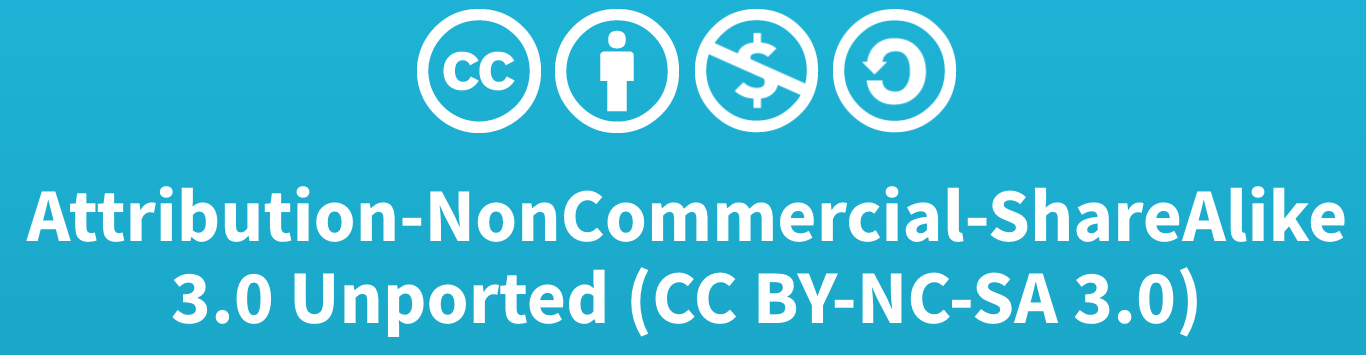
\includegraphics[scale=0.1]{CC-BY-NC-SA.png}
%   \end{center}
%   Si no s'especifica el contrari, les figures han estat extretes de la Wikipedia o altres fonts d'Internet que permeten la seva reutilització. Les figures que inclouen compostos químics, sempre que hagi estat possible, s'han creat amb el paquet \LaTeX 
%    \textsf{chemfig}.}
% \end{center}
\logos

\tableofcontents

% nova organització per al curs de química en enginyeria de l'automoció

\chapter{Les propietats i el comportament dels gasos}

\tableofcontents\newpage

L'estudi dels gasos és fonamental per a comprendre el comportament de la matèria en estat gasós. Aquests conceptes són claus tant en la química moderna com en l'aplicació industrial. Les lleis dels gasos proporcionen una base per descriure el comportament macroscòpic dels gasos en funció de la temperatura, el volum i la pressió. Aquestes lleis són fonamentals per a la comprensió de molts processos químics i físics, com ara la termodinàmica, la cinètica química i la química de superfícies.
 
\section{Les lleis dels gasos} 
En general, el volum d'un gas està determinat per la seva temperatura i la pressió que suporta. Existeix una relació matemàtica entre aquests paràmetres, que s'expressa com l'\textbf{equació d'estat}:
\begin{equation}
V = V(T, P, n), 
\end{equation}
on $V$ és el volum, $T$ és la temperatura, $P$ la pressió, i $n$ el nombre de mols del material. Es tracta d'una equació que pot ser molt complexa i específica per a líquids i sòlids, però en el cas dels gasos tots ells tenen un comportament molt similar. Això és degut a que en l'estat gas, les molècules són mes independents entre elles i, per tant, la seva naturalesa molecular no afecta substancialment al comportament del tot. 

\begin{mybox}[title={De partícules i mols de partícules}]
    El mol és la unitat bàsica del Sistema Internacional per mesurar la quantitat de substància, i s'utilitza per comptar partícules com àtoms, molècules o ions. Un mol conté exactament \(N_0=6,022 \times 10^{23}\) entitats elementals, un valor conegut com el nombre d'Avogadro. Aquesta constant permet connectar les dimensions microscòpiques (com la massa i el nombre de partícules) amb mesures macroscòpiques utilitzades en els experiments químics. Per exemple, un mol d'àtoms de carboni-12 (que representarem per \isotope*{12,C}, a partir d'ara) té una massa de 12 grams, facilitant així la relació entre l'estructura atòmica i la pràctica de la química.
\end{mybox}
    
\subsection{Pressió i força}

Un dispositiu típic per mesurar la pressió és el baròmetre, que utilitza una columna de mercuri per determinar la pressió atmosfèrica.

\begin{figure}[h]
    \centering
    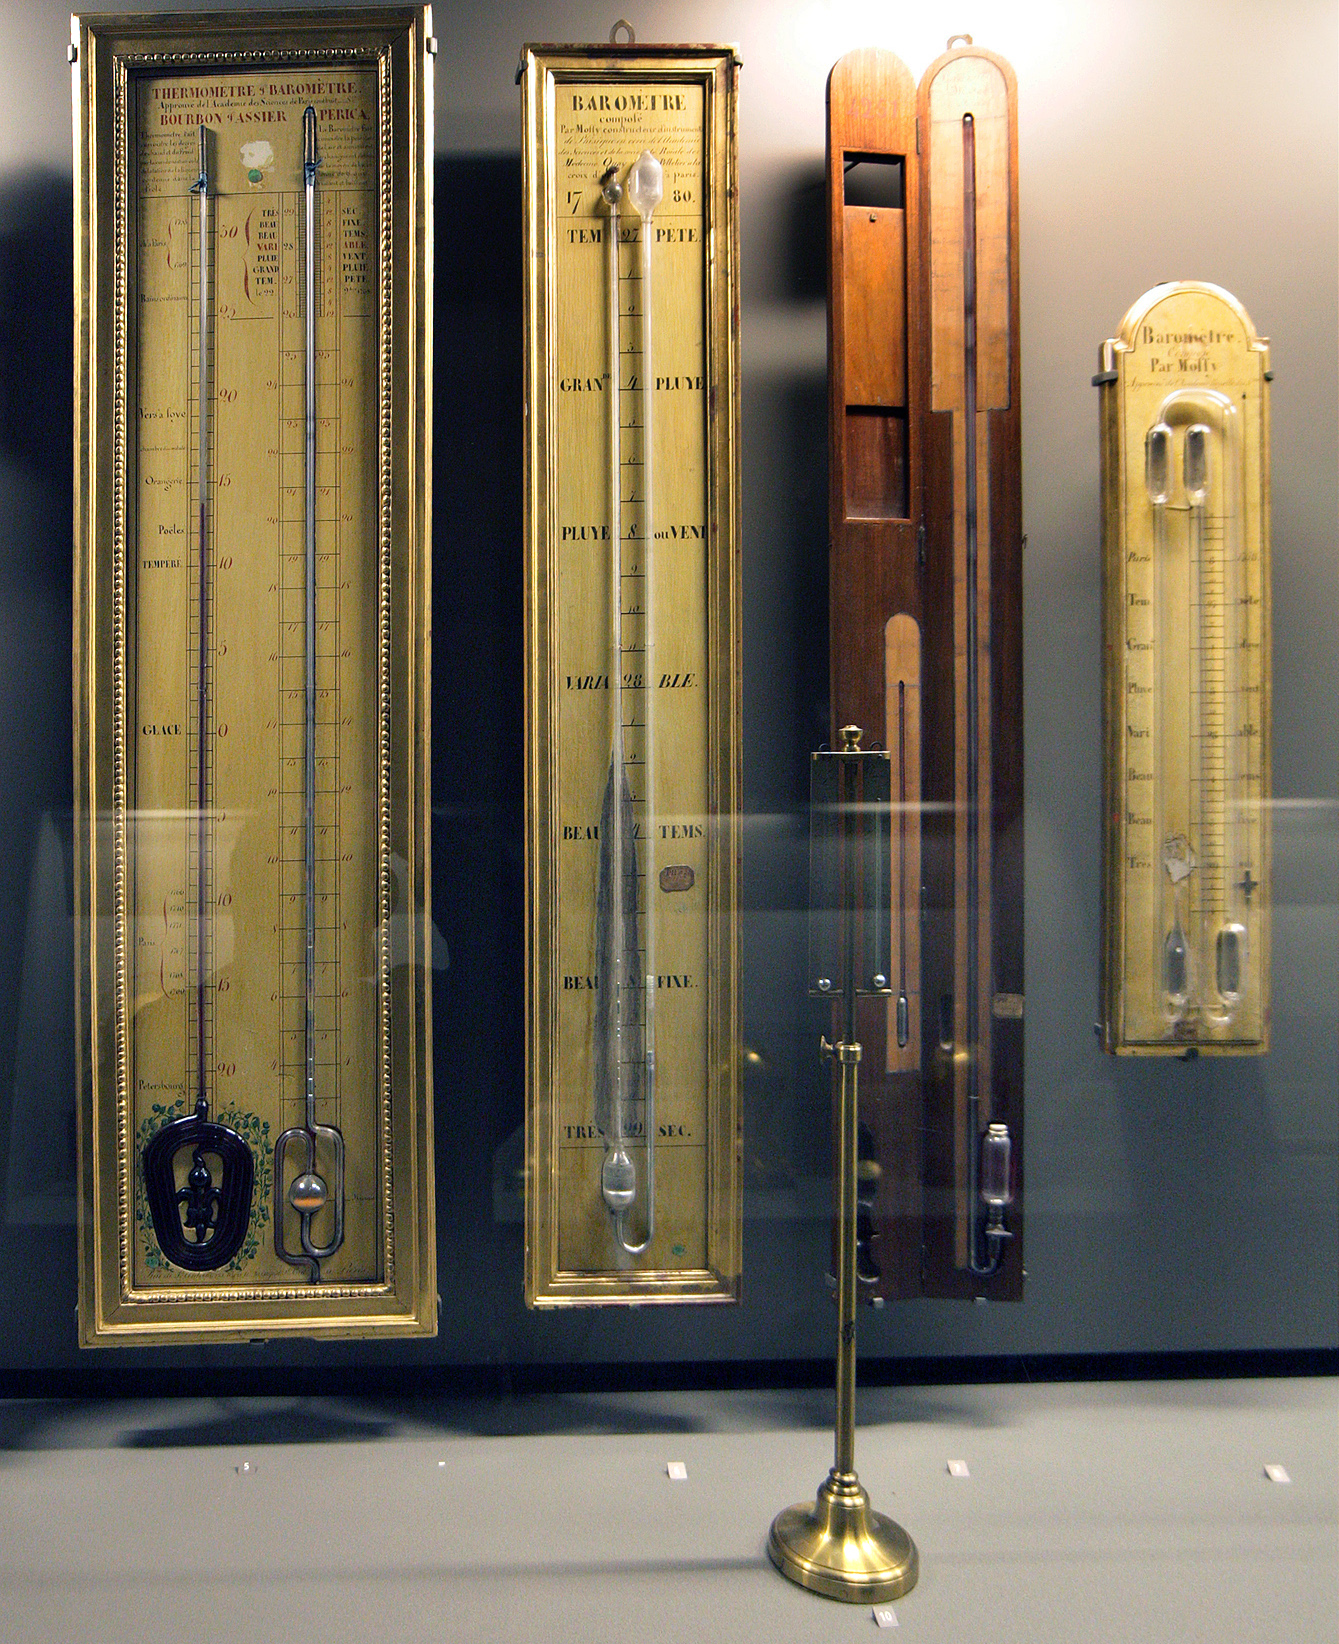
\includegraphics[width=0.33\textwidth]{Old-barometers.jpg}
    \includegraphics[width=0.33\textwidth]{Manometre.png}
    \caption[Baròmetre i Manòmetre diferencial]{El baròmetre (esquerra) utilitza una columna de mercuri per determinar la pressió atmosfèrica. Un manòmetre diferencial (dreta) mesura la diferència entre les pressions externes i d'un determinat gas.}
    \label{fig:Manometre}
    \end{figure}

La pressió és definida com la força per unitat d'àrea que un gas exerceix sobre les parets del recipient que el conté. S'expressa comunament en unitats com pascals (\si\pascal) o atmosferes (\si\atm). Matemàticament:
\begin{equation}
\text{Pressió} = \frac{\text{Força}}{\text{Àrea}} = \frac{\text{massa} \times \text{acceleració}}{\text{Àrea}} = \frac{\text{massa} \times \text{acceleració}}{\text{Volum / alçada}} 
\end{equation}
Per tant, la pressió es calcula com:
\begin{equation}
P = \rho \cdot g \cdot h,
\end{equation}
on $\rho$ és la densitat, $g$ l'acceleració gravitatòria i $h$ l'alçada.

Calculem ara què és una atmosfera quan s'expressa en funció de força per àrea unitaria. Considerem una columna de mercuri amb una alçada de 760 mm. Sabem que la densitat del mercuri és $13.6 \cdot 10^3 \si{\kg\per\meter\tothe{3}}$ i l'acceleració gravitatòria és $9.8 \si{\meter\per\square\second}$.  Considerem un tub baromètric la superfície de secció transversal del qual és 1 \si{\square\cm}. Aleshores, la força que exerceix la columna de mercuri sobre aquesta superfície és igual a la massa del mercuri que es troba al tub, multiplicada per l'acceleració deguda a la gravetat. A la vegada, la massa del mercuri que està en el tub és el volum del mercuri multiplicat per la seva densitat a $0^{\circ}\text{C}$. Així doncs, es té:

\[
\text{força} = 
\]
\[
= \text{densitat del Hg} \times \text{alçada} \times \text{àrea} \times \text{acceleració}
\]
\[
= 13,59 \, \frac{\si\g}{\si{\cubic\cm}} \times 76,00 \, \si{\cm} \times 1,000 \, \si{\square\cm} \times 980,7 \, \frac{\si{\cm}}{\si{\s}^2}
\]
\[
= 1,013 \times 10^6 \, \si\g \cdot \frac{\si\cm}{\si{\s}^2} = 10,13 \, \si\kg \cdot \frac{\si\m}{\si{\s^2}}
\]
\[
= 10,13 \si{\newton}.
\]

\begin{longtable}{cc}
    \hline
    \textbf{Unitat de Pressió} & \textbf{Pressió (en relació a 1 atm)} \\ \midrule\endhead
    Atmosfera (atm) & 1 atm \\ 
    Pascal (Pa) & \( 101325 \, \text{Pa} \) \\ 
    Bar & \( 1.01325 \, \text{bar} \) \\ 
    Mil·límetre de mercuri (mmHg) & \( 760 \, \text{mmHg} \) \\ 
    Torra (Torr) & \( 760 \, \text{Torr} \) \\ 
    Pounds per square inch (psi) & \( 14.696 \, \text{psi} \) \\ 
    Kilopascal (kPa) & \( 101.325 \, \text{kPa} \) \\    \bottomrule
    \caption{Comparació de les unitats de pressió amb 1 atmosfera}
    \end{longtable}

    \begin{mybox}[title=La pressió dels pneumàtics]
        Les pressions en els pneumàtics normalment es donen en psi (\si{\psi}), però és important saber si aquesta mesura és relativa a la pressió atmosfèrica o absoluta. Els manòmetres dels pneumàtics mesuren pressió relativa, excloent la pressió atmosfèrica.
    
        Si un pneumàtic s'ha d'omplir a \qty{35}{\psi} de pressió absoluta, cal sumar la pressió atmosfèrica \qty{14.7}{\psi}, obtenint \qty{20.3}{\psi} en el manòmetre. Una mala interpretació pot portar a inflar o desinflar inadequadament el pneumàtic, afectant la seguretat i el rendiment del vehicle.
        \end{mybox} 

Aquesta és la força que exerceix una columna de mercuri de 760 mm d'alçada i d'1 $\text{cm}^2$ de superfície de secció transversal. Per tant, és també la força per unitat de superfície (un centímetre quadrat) que correspon a la pressió d'una atmosfera.   
 Així, es té que:

\[
1 \, \si{\atm} = 760,0 \, \si\mmHg= 760 \,\si\Torr
= 1,013 \times 10^6 \, \si{\dyn\per\square\cm} = 1,013 \times 10^5 \, \si{\newton\per\square\meter}.
\]

Els gasos es comporten segons certes lleis empíriques que han estat establertes experimentalment. Aquestes lleis condueixen finalment a la formulació de la llei dels gasos ideals.

\begin{mybox}[title=Quantitats intensives i extensives]
    Les propietats es poden classificar entre extensives (m, V, ...) o intensives (T, P, capacitat calorífica ...), segons depenguin de la quantitat de substància o no. La raó entre dues propietats extensives és sempre intensiva: $\delta = \frac{m}{V}$; $\nu = \frac{V}{m}$. Només necessitem dues propietats intensives per determinar l'estat d'un gas ($P$ i $T$) i, per tant, amb tres variables intensives podem construir una equació d'estat: 
    \[F(P,V_{\rm m},T)=0\]
    
    La mesura d'una propietat per mol s'anomena valor molar d'aquesta variable. Per exemple $V_{\rm m} = \frac{V}{n}$. La Taula \ref{tab:volum_molar} mostra els valors del volum molar per a diferents gasos. 
\end{mybox}

\begin{table}[h!]
    \centering
    \begin{tabular}{l S}
    \hline
    \textbf{Gas} & \textbf{Volum molar (\si{\litre})} \\
    \hline
    \ch{He}  & 22.434 \\
    \ch{Ar}  & 22.397 \\
    \ch{H2}  & 22.433 \\
    \ch{N2}  & 22.402 \\
    \ch{O2}  & 22.397 \\
    \ch{CO2} & 22.260 \\
    \ch{NH3} & 22.079 \\
    \hline
    \end{tabular}
    \caption{Valors del volum molar (\si{\liter}) per a diferents gasos\cite{anonymous_principles_2012}.}
    \label{tab:volum_molar}
    \end{table}

\subsection{Llei de Boyle}

Robert Boyle (1627-1691) va notar, fent servir un manometre com el de la Figura \ref{fig:Manometre}, que existia una determinada llei de proporcionalitat entre la pressió exercida sobre un gas i el volum d'aquest
\begin{figure}[h]
\centering
\includegraphics[scale=0.10]{Boyle.png}
\caption{Experiment de Boyle i llei de proporcionalitat entre la pressió exercida sobre un gas i el seu volum.}
\label{fig:Boyle}
\end{figure}
Va descobrir que el producte entre el volum i la pressió és una constant, la qual cosa duu a que sota dues condicions diferents de pressió els volums es comporten de la següent manera per al mateix gas a una temperatura donada:
\[
\frac{V_1}{V_2}=\frac{P_2}{P_1}
\]

Així, la pressió \( P \) d'un gas és inversament proporcional al seu volum \( V \):
\begin{equation}
    P V = \text{constant}
\end{equation}
On \( P \) s'expressa en \si{Pa} (pascals) i \( V \) en \si{m^3}.

\subsection{Llei de Charles}

Jacques Charles (1787) i posteriorment Gay-Lussac van trobar que per a una mateixa pressió, la relació $\frac{V_{100 \si\degreeCelsius}}{V_{0 \si\degreeCelsius}}$ era identica per a tots els gasos (1.376).

Això duu a extrapolar fàcilment el comportament dels gasos i determinar el zero absolut de temperatura segons el gràfic \ref{fig:zeroabsolut}. Lord Kelvin (1848) va proposar usar el punt d'intersecció del gràfic amb la línia de les abcisses com a origen d'una nova escala de temperatura: $T/\rm{K} = t/\si\degreeCelsius + 273.15$.\marginnote{en realitat s'usa 273.16, que és el punt triple de l'aigua, temperatura a la qual coexisteixen en equilibri aigua, gel i vapor en un recipient tancat}
\begin{figure}[h]
\centering
\includegraphics[scale=1.0]{zeroabsolut.png}
\caption{Gràfic del zero absolut a partir de la llei de Charles i Gay-Lussac.}
\label{fig:zeroabsolut}
\end{figure}

La llei de Charles afirma que, a pressió constant, el volum d'un gas és directament proporcional a la seva temperatura absoluta \( T \):
\begin{equation}
    \frac{V}{T} = \text{constant}
\end{equation}
On \( T \) es mesura en \si{K} (Kelvins).

\begin{mybox}[title=Amortidors]
    Utilitzem les lleis de Boyle i Charles per explicar com funciona un amortidor o una barra d'amortidor omplerta de gas en la suspensió d'un cotxe i per què s'utilitza un líquid en les línies de frens en lloc d'un gas.

    El pistó senzill és un sistema idealitzat on una quantitat fixa de gas queda atrapada dins d'una cambra tancada per un pistó en contacte amb l'atmosfera. La cambra funciona com un sistema tancat, fixant el nombre de molècules de gas dins del sistema, definit com el gas atrapat dins de la cambra. La resta de l'aparell permet que la temperatura, la pressió i el volum variïn. Si es manté constant una d'aquestes variables (temperatura, pressió o volum), es pot explorar la relació entre les altres dues variables mitjançant experiments.
\begin{center}
    \begin{tikzpicture}[centered]
      \def\Ra{0.5}
      \def\Rb{1.0}
      \def\ra{0.1}
      \def\rb{0.2}
      \def\w{0.08} % wall thickness
      \def\x{2.9}  % piston position
      \def\L{3.7}  % container length
      \def\l{2.2}  % piston arm length
      \def\v{0.68} % velocity
      
      % WALL
      \draw[wall]
        (0,\Rb) -- (0,-\Rb) --++ (\L,0) arc (-90:90:{\Ra} and {\Rb}) -- cycle;
      \draw[walldark] (0,0) ellipse ({\Ra} and \Rb);
      
      % SHELL
      \draw[walldark]
        (0,\Rb) rectangle++ (\L,\w);
      \draw[walldark]
        (0,-\Rb) rectangle++ (\L,-\w);
      \draw[walldark]
        (\L,\Rb+\w) arc (90:-90:{\Ra+\w} and {\Rb+\w}) --++ (0,\w) arc (-90:90:{\Ra} and {\Rb}) -- cycle;
      \draw[walldark]
        (0,\Rb) arc (90:270:{\Ra} and {\Rb}) --++ (0,-\w) arc (-90:-270:{\Ra+\w} and {\Rb+\w}) -- cycle;
      
      % PISTON
      \draw[walldark]
        (\x,\Rb) arc (90:270:{\Ra} and {\Rb}) --++ (-2*\w,0) arc (-90:-270:{\Ra} and {\Rb}) -- cycle;
      \draw[piston] (\x,0) ellipse ({\Ra} and \Rb);
      \draw[piston]
        (\x,\rb) arc (90:270:{\ra} and {\rb}) --++ (\l,0) --++ (0,2*\rb) -- cycle;
      \draw[walldark] (\x+\l,0) ellipse ({\ra} and \rb);
      
      % LABELS
      \draw[->,very thick,orange!90!black] (\x,0.5*\Rb) --++ (0.2*\L,0)
        node[right=-2,orange!90!black] {$P$};
      \node[right,blue!60!black,above] at (\L/2-\Ra,\Rb+\w) {$V$, $P$, $T$};
      \draw[<-,thick,blue!60!black] (\x,0.7*\Rb) to[in=-30] (\x,1.2*\Rb)
        node[below=3,above left] {$A$};
      
      % GAS PARTICLE
      \pic at (-0.12*\x, 0.2*\Rb) {gasparticle={vec={ -40:0.7*\v}}};
      \pic at (-0.07*\x,-0.5*\Rb) {gasparticle={vec={  48:0.6*\v}}};
      \pic at ( 0.00*\x, 0.3*\Rb) {gasparticle={vec={ 105:0.6*\v}}};
      \pic at ( 0.05*\x,-0.5*\Rb) {gasparticle={vec={-100:0.6*\v}}};
      \pic at ( 0.08*\x, 0.0*\Rb) {gasparticle={vec={  70:0.5*\v}}};
      \pic at ( 0.07*\x, 0.7*\Rb) {gasparticle={vec={ -10:0.9*\v}}};
      \pic at ( 0.15*\x,-0.2*\Rb) {gasparticle={vec={  30:0.7*\v}}};
      \pic at ( 0.20*\x,-0.8*\Rb) {gasparticle={vec={ -10:0.6*\v}}};
      \pic at ( 0.35*\x, 0.6*\Rb) {gasparticle={vec={-110:0.7*\v}}};
      \pic at ( 0.35*\x,-0.6*\Rb) {gasparticle={vec={ 140:0.4*\v}}};
      \pic at ( 0.40*\x, 0.9*\Rb) {gasparticle={vec={ -40:0.7*\v}}};
      \pic at ( 0.43*\x,-0.2*\Rb) {gasparticle={vec={  75:0.8*\v}}};
      \pic at ( 0.50*\x, 0.5*\Rb) {gasparticle={vec={-170:0.5*\v}}};
      \pic at ( 0.52*\x,-0.7*\Rb) {gasparticle={vec={ 120:0.6*\v}}};
      \pic at ( 0.60*\x, 0.4*\Rb) {gasparticle={vec={ -80:0.5*\v}}};
      \pic at ( 0.63*\x,-0.6*\Rb) {gasparticle={vec={  42:0.5*\v}}};
      \pic at ( 0.65*\x,-0.2*\Rb) {gasparticle={vec={ 150:0.6*\v}}};
      \pic at ( 0.68*\x,-0.8*\Rb) {gasparticle={vec={ 190:0.5*\v}}};
      \pic at ( 0.72*\x, 0.8*\Rb) {gasparticle={vec={ 160:0.5*\v}}};
      \pic at ( 0.72*\x, 0.3*\Rb) {gasparticle={vec={  80:0.6*\v}}};
      
    \end{tikzpicture}
  \end{center}
    
    El pistó no es mourà quan la pressió dins de la cambra sigui igual a la pressió exterior. Aquesta condició d'igualtat de pressions estableix la posició d'equilibri del pistó. Si es manté constant la temperatura, la pressió dins del sistema es pot variar canviant la força externa aplicada al pistó. Com que l'àrea de la superfície del pistó en contacte amb el sistema és invariable, l'aplicació d'una força exterior més gran augmenta la pressió externa. El sistema respon reduint el volum fins que la pressió interna s'iguala a la pressió externa.
    
    La teoria cinètica molecular ens diu que l'origen de l'augment de la pressió és un increment en el nombre de col·lisions entre les molècules del gas i les parets de la cambra en un temps determinat. Fixant la temperatura, es fixa l'energia cinètica mitjana del sistema i, per tant, l'energia mitjana de cada col·lisió. Com que no podem donar més energia cinètica a les partícules escalant el gas per combatre l'augment de la pressió externa, el gas s'ha de forçar a augmentar el nombre de col·lisions, i ho fa disminuint el volum. Això indica que la pressió i el volum tenen una relació inversa, tal com es descriu a la llei de Boyle:
    
    \[
    p\propto \frac{1}{V}  
    \]
    
    Si es manté constant la pressió externa, es pot explorar la relació entre el volum i la temperatura utilitzant el pistó senzill. Si s'escalfa el gas dins de la cambra, l'energia cinètica mitjana de les partícules augmenta, segons la teoria molecular cinètica. Això fa que cada col·lisió sigui més energètica i que el nombre de col·lisions entre les partícules del gas i la superfície interna del pistó augmenti en un interval de temps donat. Amb l'augment de les col·lisions, es genera una major força sobre el pistó, que ha de moure's cap amunt per aconseguir un nou punt d'equilibri.

    \[
      V \propto T
      \]

      Quan el cotxe passa per un sot, l'impacte es transfereix gairebé completament al vehicle. Si aquesta energia no s’absorbeix, els passatgers notarien una sacsejada brusca. Els amortidors de gas ajuden a suavitzar aquest impacte seguint les lleis dels gasos.

Quan l’amortidor rep el cop, un pistó comprimeix el gas dins d’una càmera tancada. Això augmenta la pressió perquè les partícules de gas xoquen més sovint amb les parets. Part de l'energia de l'impacte es converteix en pressió i temperatura. El gas circula per petites obertures dins de l’amortidor, es refreda i dissipa l’energia. A més, l’aire exterior refresca l’amortidor.

Finalment, la molla retorna l’amortidor a la seva posició original, permetent que el gas torni a omplir la càmera sense gastar gaire energia. Això permet que l’amortidor sigui reutilitzat en cada impacte.
    
\end{mybox}


      


\subsection{Llei d'Amonton (o de Gay-Lussac)}
La llei de Gay-Lussac és una llei dels gasos que estableix que la pressió \( P \) exercida per un gas (d'una massa donada i mantingut a volum constant) varia directament amb la temperatura absoluta del gas:
\begin{equation}
    T \propto P \quad \text{o} \quad P = \text{constant} \times T
\end{equation}
En altres paraules, si un gas ideal està confinat en un recipient amb volum constant i s'incrementa la temperatura, la pressió augmentarà proporcionalment a la temperatura.

%\begin{exr}
    Un conductor comprova la pressió dels pneumàtics pel matí aviat, quan la temperatura és de 15\si\degreeCelsius, i és de 1.3$\times$10$^5$ Pa. Al migdia la temperatura és 15 graus més elevada. Quina és la pressió dels pneumàtics ara?.
    \end{exr}

%    \begin{exr}
        Dalt de l'Everest, la pressió atmosfèrica és de 0,33 atm i la temperatura de 50 sota zero. Quina és la densitat de l'aire si en CN és de 1.29\si{\gram\per\deci\meter\tothe{3}}?.
        \end{exr}
    \lct{


Sabem que la densitat de l'aire en condicions normals (CN) és:

\[
\rho_{\text{CN}} = \SI{1.29}{\gram\per\deci\meter\cubed}
\]

Les condicions a dalt de l’Everest són:

\begin{itemize}
    \item Pressió atmosfèrica: \( P = \SI{0.33}{\atm} \)
    \item Temperatura: \( T = \SI{-50}{\celsius} = \SI{223}{\kelvin} \)
    \item Condicions normals (CN):
    \begin{itemize}
        \item Pressió normal: \( P_{\text{CN}} = \SI{1}{\atm} \)
        \item Temperatura normal: \( T_{\text{CN}} = \SI{273}{\kelvin} \)
    \end{itemize}
\end{itemize}

Sabem que la densitat d'un gas està relacionada amb la pressió i la temperatura segons l'expressió:

\[
\frac{\rho}{\rho_{\text{CN}}} = \frac{P}{P_{\text{CN}}} \times \frac{T_{\text{CN}}}{T}
\]

Aïllant \( \rho \):

\[
\rho = \rho_{\text{CN}} \times \frac{P}{P_{\text{CN}}} \times \frac{T_{\text{CN}}}{T}
\]

Substituïm els valors donats:

\[
\rho = (\SI{1.29}{\gram\per\deci\meter\cubed}) \times \frac{\SI{0.33}{\atm}}{\SI{1}{\atm}} \times \frac{\SI{273}{\kelvin}}{\SI{223}{\kelvin}}=\SI{0.52}{\gram\per\deci\meter\cubed}
\]

    }
      


\begin{mybox}[title=La llei de Gay-Lussac i els pneumàtics de cursa]
 En curses, els pilots sovint fan girs bruscs amb els cotxes d'un costat a l'altre de la pista darrere del cotxe de seguretat abans que s'agit\'i la bandera verda. Tamb\'e permeten que es formin espais entre el cotxe perseguit i el seu, per despr\'es accelerar bruscament i fer derrapar les rodes motrius.

En competicions de {\em drag racing}, \`es habitual que els cotxes facin un escalfament important de les rodes motrius mitjan\c{c}ant una fricci\'o intensa a la l\'inia de sortida. En la F\'ormula 1, sovint es poden veure cotxes al paddock abans de la classificaci\'o o de la cursa amb escalfadors el\`ectrics de pneum\`atics embolicant les rodes. En tots aquests casos, els equips i pilots escalfen els pneum\`atics per optimitzar l'adher\`encia i la pressi\'o.

Suposem que els pneum\`atics es van omplir a \qty{40}{\psi} la nit abans d'una cursa, quan la temperatura era de \qty{15}{\celsius} (\qty{288}{\kelvin}). Al mat\'i, es col·loquen a la zona de preparaci\'o i s'escalfen sota el sol fins a \qty{30}{\celsius} (\qty{303}{\kelvin}). Aplicant la llei de Gay-Lussac:

\begin{equation}
    \frac{P_1}{T_1} = \frac{P_2}{T_2}
\end{equation}

Substituint les dades:

\begin{equation}
    \frac{\qty{40}{\psi}}{\qty{288}{\kelvin}} = \frac{P_2}{\qty{303}{\kelvin}}
\end{equation}

que ens dóna: $P_2 = \qty{42.1}{\psi}$.

Aquesta difer\`encia pot semblar petita, per\`o en curses, unes d\'ecimes de \si{\psi} poden alterar significativament l'al\c{c}ada del vehicle, la mida de la zona de contacte amb la pista i la rigidesa efectiva de la suspensi\'o.

A m\'es, la temperatura d'un pneum\`atic de curses en plena acci\'o pot arribar a uns  \qty{373}{\kelvin}. Aix\`o augmenta encara m\'es la pressi\'o fins a \qty{51.8}{\psi}, la qual cosa ha de ser considerada abans de muntar els pneum\`atics al cotxe.

El mateix efecte es pot observar en els cotxes convencionals. Si s'omplen els pneumàtics a \qty{35}{\psi} en un dia calorós d'estiu a \qty{32}{\degC} (\qty{305}{\kelvin}), la pressió disminuirà en un dia fred d'hivern amb una temperatura de \qty{-7}{\degC} (\qty{266}{\kelvin}) fins a \qty{30.5}{\psi}.

Aix\`o suposa una disminuci\'o d'entre \qty{4}{\psi} i \qty{5}{\psi}, \`es a dir, una reducci\'o de gaireb\'e un \qty{13}{\percent}!!
\end{mybox}

\subsection{Llei dels Gasos Ideals}
Combinant les tres lleis anteriors, obtenim la llei dels gasos ideals:
\begin{equation}
    P V = n R T
\end{equation}
o bé:
\[\frac{P V_{\rm m}}{T}= cnt = R\]

On:
\begin{itemize}
    \item \( P \) és la pressió en \si{Pa}
    \item \( V \) és el volum en \si{m^3}
    \item \( n \) és el nombre de mols
    \item \( R \) és la constant dels gasos, amb valor \( \SI{8.314}{J.mol^{-1}.K^{-1}} \)
    \item \( T \) és la temperatura en \si{K}
\end{itemize}

Per tal de determinar la $R$ no podem simplement calcular el quocient $\frac{P V_{\rm m}}{T}$ per a qualsevol gas, ja que cadascun d'ells donarà un valor diferent (només és vàlida l'expressió per a un gas ideal!). Veure la Figura \ref{fig:R2}.
\begin{marginfigure}
\centering
\includegraphics[scale=1.0]{R2.png}
\caption[Determinació de la constant dels gasos $R$]{R es pren com al valor límit de la fracció $\frac{P V_m}{T}$ per a tots els gasos: 
$R=\lim_{P \to 0} \frac{P V_{\rm m}}{T}= 0.08205 \frac{{\rm atm l}}{{\rm mol K}}$
}
\label{fig:R2}
\end{marginfigure}

%\begin{exr}
    Calcular el volum molar d'un gas ideal a condicions normals (1 atm i 0\si\degreeCelsius).
    \end{exr}

\begin{mybox}[title=Condicions normals (o estàndard) de temperatura i pressió]
    En química, la \href{https://iupac.org/}{IUPAC} va establir la temperatura i la pressió estàndard o normal (en anglès, \emph{standard temperature and pressure} com a STP) com una temperatura de \qty{273.15}{\kelvin} (\qty{0}{\degC}, \qty{32}{\degF}) i una pressió absoluta de \qty{100}{\kilo\pascal} (\qty{14.504}{\psi}, \qty{0.986}{\atm}, \qty{1}{\bar}). 
    
    Hi ha certa confusió internacional entre els termes normal i estàndard. A Europa les condicions estàndard fan referència a una temperatura de \qty{298.15}{\kelvin} (\qty{25}{\degC}, \qty{77}{\degF}) i una pressió absoluta de \qty{1}{\atm} (\qty{101.325}{\kilo\pascal}). El terme equivalent en anglès és \emph{standard ambient temperature and pressure} (SATP). 
    
    L'STP i el SATP no s'han de confondre amb l'estat estàndard comunament utilitzat, com veurem més endavant en aquest curs, en les avaluacions termodinàmiques de l'energia lliure de Gibbs d'una reacció.

    Podeu veure una interessant referència sobre aquest tema a \cite{doiron_20_2007}.
\end{mybox}

%\begin{exr}
    Quant gas hi ha en una mostra de volum \qty{0.5}{\deci\meter\tothe{3}}, a \qty{80}{\degC} i \qty{800}{\torr} de pressió?
    \end{exr}

%\begin{exr}{}
Pots calcular el volum ocupat per molècula en un gas ideal a CN?. Es troben dues molècules molt freqüentment en un gas a baixa pressió?
\end{exr}


\subsection{Llei de Dalton}
La llei de les pressions parcials de Dalton estableix que la pressió total d'una mescla de gasos ideals és igual a la suma de les pressions parcials dels gasos individuals en la mescla. Matemàticament, es pot expressar així:

\[
P_{\text{total}} = P_1 + P_2 + P_3 + \cdots + P_n
\]

on \(P_{\text{total}}\) és la pressió total de la mescla, i \(P_1, P_2, \dots, P_n\) són les pressions parcials dels diferents gasos presents a la mescla.

La pressió parcial d'un gas és la pressió que exerciria aquest gas si ocupés tot el volum per si sol, a la mateixa temperatura.
  
%\begin{exr}{Pressió parcial \ch{PCl5} en una mescla (adaptat de \cite{mahan_quimica_1997})}
    Una mostra de \ch{PCl5}, que pesa \SI{2.69}{\gram}, es va col·locar en un flascó d'\SI{1.00}{\litre} i es va evaporar completament a una temperatura de \SI{250}{\celsius}. La pressió observada a aquesta temperatura va ser \SI{1.00}{\atm}. Existeix la possibilitat que una part del \ch{PCl5} s'hagi dissociat d'acord amb l'equació:

\begin{reaction}
PCl5(g) -> PCl3(g) + Cl2(g)
\end{reaction}

Quines són les pressions parcials del \ch{PCl5}, \ch{PCl3} i \ch{Cl2} en aquestes condicions experimentals?
\end{exr}
\lct{
    La solució d'aquest problema implica diverses etapes. Per determinar si s'ha dissociat una part del \ch{PCl5}, calculem primerament la pressió que s'hauria observat si no s'hagués dissociat el \ch{PCl5}. Això es pot calcular a partir del nombre de mols de \ch{PCl5} utilitzats, juntament amb el volum i la temperatura del flascó. Com que el pes molecular del \ch{PCl5} és \SI{208}{\gram\per\mole}, el nombre de mols de \ch{PCl5} inicialment presents en el flascó és:

\[
n = \SI{2.69}{\gram}\cdot \frac{1\si{\mole}}{\SI{208}{\gram}} = 0.0129\si{\mole}.
\]

La pressió corresponent a aquest nombre de mols seria:

\[
P = \frac{nRT}{V} = \frac{(0.0129\si{\mole})(\SI{0.082}{\liter\atm\per\mole\per\kelvin})(\SI{523.15}{\kelvin})}{\SI{1.00}{\liter}} = \SI{0.553}{\atm}.
\]

Com que la pressió observada és superior a aquesta, s'ha de produir certa dissociació del \ch{PCl5}. Aplicant la llei de les pressions parcials, podem escriure:

\begin{equation}
P_{\ch{PCl5}} + P_{\ch{PCl3}} + P_{\ch{Cl2}} = P_t = \SI{1.00}{\atm}.
\label{eq:daltonpcl}
\end{equation}

Ara observem que:


Atès que es produeix un mol de \ch{PCl3} i un mol de \ch{Cl2} per cada mol de \ch{PCl5} dissociat,
\[
P_{\ch{Cl2}} = P_{\ch{PCl3}}, \quad P_{\ch{PCl5}} = \SI{0.553}{\atm} - P_{\ch{Cl2}}.
\]
i podem reescriure l'Equació \ref{eq:daltonpcl} com:

\[
\SI{0.553}{\atm} - P_{\ch{Cl2}} + P_{\ch{Cl2}} + P_{\ch{Cl2}} = \SI{1.00}{\atm}.
\]

Resolent, obtenim:

\[
P_{\ch{Cl2}} = \SI{0.447}{\atm},
\]

i

\[
P_{\ch{PCl3}} = \SI{0.447}{\atm}, \quad P_{\ch{PCl5}} = \SI{0.106}{\atm}.
\]
}


\begin{mybox}[title=Nitrogen als pneumàtics?] 
  Els pneumàtics solen estar plens d’aire, que té la mateixa proporció d’oxigen i nitrogen. Quan es recorre a nitrogen pur per inflar els pneumàtics, es redueix la pressió parcial d’oxigen i s’augmenta la de nitrogen. Això té dos avantatges menors per a la conducció quotidiana. Primer, en reduir la pressió parcial d’oxigen, es disminueix l’oxidació que pot deteriorar el cautxú del pneumàtic.

El segon avantatge és la reducció de la quantitat d’aigua dins del pneumàtic. L’aire conté sempre una certa quantitat de vapor d’aigua, i els compressors que inflen els pneumàtics solen introduir aire humit. Aquesta aigua pot vaporitzar-se parcialment dins del pneumàtic i, com que la temperatura varia mentre es condueix, provoca fluctuacions de pressió. A més, l’aigua pot contribuir a la degradació química dels pneumàtics i les llantes. Inflant-los amb nitrogen sec, s’evita la presència d’aigua líquida i gasosa, eliminant aquests inconvenients.
\end{mybox}

\section{Teoria Cinètica dels Gasos}

Per tal de relacionar aquestes descobertes amb l'estructura atòmica de la matèria, ens cal introduir una teoria que representi els gasos de forma extremadament simple: un \textit{model}. En el nostre cas (veure Figura \ref{fig:TeoriaCinetica}),
\begin{itemize}
\item el gas és format per partícules que es comporten com a punts de massa, i
\item a més de no col·lidir, no exerceixen força les unes sobre les altres.
\end{itemize}
\begin{figure}[h]
\centering
\includegraphics[scale=0.2]{TeoriaCinetica.png}
\caption{Representació del moviment de les partícules en un gas ideal.}
\label{fig:TeoriaCinetica}
\end{figure}

%\begin{exr}{}
Pots calcular el volum ocupat per molècula en un gas ideal a CN?. Es troben dues molècules molt freqüentment en un gas a baixa pressió?
\end{exr}


Aquesta teoria, de forma relativament simple, ens permet expressar la pressió que s'exerceix sobre les parets d'un recipient per part del gas que conté segons:
\[
PV=\frac{2}{3} \left< E_c \right> = \frac{2}{3} N_0 \left< \frac{mc^2}{2} \right>
\]
on $N_0$ és el número d'Avogadro.

D'aquí s'extreuen resultats interessants, com que l'energia cinètica translacional d'un mol de gas és 
\[\left<E_c\right>=N_0 \frac{m <c^2>}{2}=\frac{3}{2} RT\] 
o bé, si dividim pel número d'Avogadro a esquerra i dreta obtenim la constant dels gasos per molècula a partir de l'energia cinètica per molècula (constant de Boltzmann $k$): 
\[\frac{m <c^2>}{2}=\frac{3}{2} kT\]
Aquest resultat ens diu que si dos gasos tenen la mateixa $T$, les seves molècules tenen la mateixa energia cinètica promig. 


La distribució de les velocitats de les partícules d'un gas segueix la distribució de Maxwell-Boltzmann\cite{mahan_quimica_1997}:
\[
\frac{\Delta N}{N}=4 \pi \left( \frac{m}{2 \pi kT}\right)^{3/2} \underbrace{e^{-mc^2/2kT}}_{\rm Boltzmann} c^2 \Delta c
\]
El factor de Boltzmann ens diu, en aquesta equació, que a qualsevol temperatura particular, acostuma a haver moltes menys molècules amb energies altes que amb energies baixes.
\begin{figure}[h]
\centering
\includegraphics[scale=0.4]{BolzDist.png}
\includegraphics[scale=0.4]{MXDIST.png}
\caption{La distribució de Maxwell-Boltzmann per a diferents molècules i temperatures}
\label{fig:Maxwell}
\end{figure}


    


\subsection{Capacitat calorífica}

La capacitat calorífica d'una substància és la quantitat de calor en calories necessària per elevar 1\si\degreeCelsius\ la temperatura d'un gram de la substància.

De fet, això necessita precissió: no és el mateix fer aquest procés d'escalfament a volum constant que a pressió constant ($C_V$ vs $C_P$).

Si afegim calor a un gas, o bé s'expandeix (i per tant fa treball) o bé la velocitat de les seves particules augmenta.
A $V$ constant, l'escalfament produeix un increment d'energia cinètica:
\[\Delta E = \frac{3}{2} R \Delta T\]
però resulta que $\Delta E/ \Delta T$ és, justament, $C_V$ i, per tant, per a un gas monoatòmic ideal, $C_V=\frac{3}{2}R$ o, aproximadament, 3 cal/mol·grau.

En el cas de pressió constant, les partícules augmenten la seva energia cinètica i també exerceixen treball ($\Delta(PV)$):
\[\Delta(PV)=P\Delta V = P(V_2-V_1)=PV_2-PV_1\]
Per a un mol de gas, resulta que $PV=RT$ i, per tant, 
\[PV_2-PV_1=RT_2-RT_1=R\Delta T\]
Per tant, la capacitat calorífica extra pel fet de fer el procés a pressió constant és
\[\frac{\Delta (PV)}{\Delta T}=R\]
i, per tant, 
\[C_P=C_V+R 
=\frac{3}{2} R + R= \frac{5}{2}R\]
És fàcil veure que $C_P/C_V=5/3=1.67$ i podem comparar aquests coeficients per a diversos gasos monoatòmics, per tal d'establir diferències amb el seu comportament ideal (Taula \ref{tab:cpcv}).
\begin{margintable}
	\begin{center}
		\caption{Quocients de capacitat calorífica \cite{mahan_quimica_1997}.}
		\label{tab:cpcv}
		\begin{tabular}{cc|cc}
			\hline
			Gas & $C_P/C_V$ & Gas & $C_P/C_V$\\
			\hline
			He & 1.66 & \ch{H2} & 1.41 \\
			Ne & 1.66 & \ch{O2} & 1.40 \\
			Ar & 1.66 & \ch{N2} & 1.40 \\
			Kr & 1.66 & \ch{CO} & 1.40 \\
			Xe & 1.66 & \ch{NO} & 1.40 \\
			Hg & 1.66 & \ch{Cl2} & 1.36 \\
			\hline
		\end{tabular}
	\end{center}
\end{margintable}


%\begin{exr}
Perquè hi ha diferències entre els quocients de capacitat calorífica ($C_P/C_V$) de gasos monoatòmics respecte els diatòmics? (Adona't que si un gas monoatòmic ideal, pel fet d'estar només augmentant la seva energia cinètica translacional té una $C_V=\frac{3}{2}R$, es pot entendre que per a cada component (eix) necessita $\frac{1}{2}R$)
\end{exr}
\lct{
    Els quocients de la capacitat calorífica dels gasos diatòmics són molt menors que 1,67, i hem d'esbrinar la raó d'aquestes desviacions.

    Primerament, notem que $C_V$, la capacitat calorífica deguda al moviment de translació de les molècules, és igual a $\frac{3}{2}R$, i que hi ha tres components independents de velocitat associats amb el moviment de translació. Per tant, podem inferir que cadascun dels tres moviments de translació independents contribueix amb $\frac{1}{2}R$ a la capacitat calorífica molar. Sobre aquesta base, podríem esperar que, si algun altre tipus de moviment fos accessible a les molècules de gas, hi hauria més contribucions a la capacitat molar i aquestes entrarien en unitats de $\frac{1}{2}R$.
    
   A més de tenir els tres moviments de translació, una molècula diatòmica pot rotar al voltant del seu centre de massa segons dos modes mútuament perpendiculars i independents. Assignant $\frac{1}{2}R$ com la contribució de cadascun d'aquests moviments a la capacitat calorífica, tenim:
    
    \[
    C_V = \underbrace{\frac{3}{2}R}_{\text{traslació}} + \underbrace{\frac{1}{2}R + \frac{1}{2}R}_{\text{rotació}} = \frac{5}{2}R,
    \]
    
    \[
    C_P = C_V + R = \frac{7}{2}R,
    \]
    
    \[
    \frac{C_P}{C_V} = \frac{\frac{7}{2}R}{\frac{5}{2}R} = \frac{7}{5} = 1,40.
    \]
}



\subsection{Gasos no ideals}

En gasos reals, el factor de compressibilitat ve donat per
\[z=\frac{V_m}{V_{m,i}}=\frac{V_m}{RT/P}=\frac{PV_m}{RT}\]
no és 1, com succeiria a un gas ideal (veure Figura \ref{fig:FactorCompress}). En general, la desviació del comportament ideal esdevé més important quan el gas està més a prop d'un canvi de fase, com més baixa és la temperatura o com més alta és la pressió. 
\begin{figure}[h]
\centering
\includegraphics[scale=0.5]{FactorCompress.png}
\caption{Factor de compressibilitat per a diferents gasos a 0\si\degreeCelsius.}
\label{fig:FactorCompress}
\end{figure}

Per tal de millorar l'aproximació a la realitat podem considerar diferents aproximacions. 
En el desenvolupament de l'equació d'estat del gas ideal (EOS), es van fer dues hipòtesis:

\begin{itemize}
    \item El volum de les molècules de gas és insignificant en comparació amb el volum total i la distància entre les molècules.
    \item No existeixen forces atractives ni repulsives entre les molècules.
\end{itemize}

Johannes Diderick van der Waals (1873) va intentar eliminar aquestes dues hipòtesis en el desenvolupament d'una equació empírica d'estat per a gasos reals. Per tal d'eliminar la primera hipòtesi, van der Waals va assenyalar que les molècules de gas ocupen una fracció significativa del volum a altes pressions i va proposar que el volum de les molècules, denotat pel paràmetre $b$, fos restat del volum molar real, $V$, en l'Eq. (5.45), per obtenir

\[
p = \frac{RT}{V - b}
\]
on el paràmetre $b$ és conegut com el covolum i es considera que reflecteix el volum de les molècules. La variable $V_m$ representa el volum real per mol de gas.

Segons això,
\[z=\frac{PV_m}{RT}=1+\frac{b}{RT}P\]
que té una forma lineal. Aixó explicaria el cas de la molècula d'hidrogen a la Figure \ref{fig:FactorCompress}.
Però què passa amb \ch{CH4} o \ch{CO}? Val la pena pensar que són molècules que es podran trobar líquides a temperatures més baixes amb major facilitat que no pas \ch{H2}. 
Per tal d'eliminar la segona hipòtesi, van der Waals va afegir un terme correctiu, denotat per $\frac{a}{V^2}$, a aquesta equació per tenir en compte les forces atractives entre les molècules.

Tenint en compte aquestes modificacions en la inclusió de $P$ i $V$ en l'equació des gasos ideals podem arribar (no ho fem aquí) a l'equació dels gasos ideals proposada per van der Waals:
\[
\left( P + \frac{a}{{V_m}^2} \right) (V_m -b)=RT
\]
o bé
\begin{equation}
\left( P + \frac{n^2 a}{V^2} \right) (V -nb)=nRT
\label{Eq:vdW}
\end{equation}

La Taula \ref{tab:van_der_waals} mostra els valors de $a$ i $b$ per a diferents gasos.

\begin{table}[h!]
\centering
\begin{tabular}{l S[table-format=1.4] S[table-format=1.5]}
\hline
\textbf{Gas} & \textbf{\textit{a} (\si{\litre\squared\atm\per\mol\squared})} & \textbf{\textit{b} (\si{\litre\per\mol})} \\
\hline
\ch{H2}   & 0.2444 & 0.02661 \\
\ch{He}   & 0.03412 & 0.02370 \\
\ch{N2}   & 1.3900 & 0.03913 \\
\ch{O2}   & 1.3600 & 0.03183 \\
\ch{CO}   & 1.4850 & 0.03985 \\
\ch{NO}   & 1.3400 & 0.02789 \\
\ch{CO2}  & 3.5920 & 0.04267 \\
\ch{H2O}  & 5.4640 & 0.03049 \\
\hline
\end{tabular}
\caption{Constants de van der Waals per a diferents gasos.}
\label{tab:van_der_waals}
\end{table}

%\begin{exr}
Què passa segons l'Equació de van der Waals si la pressió es fa propera a zero o bé la temperatura es fa molt gran per a un gas real?   La figura mostra el factor de compressibilitat per a un mateix gas a diferents temperatures
\begin{center}        \includegraphics[scale=1.0]{FactorCompressT.png}
\end{center}
\end{exr}

\section{Les forces de van der Waals}

Les forces de van der Waals són degudes a tres contribucions:
\begin{enumerate}
\item  forces dipol-dipol.
\item Efecte de distorsió: forces d'inducció.
\item Efecte de dispersió: forces de dispersió.
\end{enumerate}


Les forces de van der Waals, que contribueixen a la pèrdua d'idealitat en una gas, són interaccions intermoleculars dèbils que apareixen entre molècules neutres. Aquestes forces inclouen:

\begin{itemize}
    \item {\bf Forces de dispersió} de London, que són degudes a fluctuacions temporals en la distribució electrònica.
    \item  {\bf Forces dipol-dipol}, que actuen entre molècules amb moments dipolars permanents.
    \item {\bf Forces d'inducció}, o forces dipol-induït, que es donen quan una molècula polar indueix un dipol en una molècula apolar.
\end{itemize}

L'energia potencial associada a les forces de van der Waals es pot aproximar mitjançant el potencial de Lennard-Jones:  

\begin{equation}
    U(r) = 4 \varepsilon \left[ \left( \frac{\sigma}{r} \right)^{12} - \left( \frac{\sigma}{r} \right)^{6} \right]
\end{equation}

on:
\begin{itemize}
    \item \( U(r) \) és l'energia potencial en funció de la distància intermolecular \( r \).
    \item \( \varepsilon \) és la profunditat del pou de potencial, representant la intensitat de la interacció.
    \item \( \sigma \) és la distància a la qual el potencial és zero.
\end{itemize}

La taula següent mostra els valors de \( \varepsilon \) i \( \sigma \) per a diferents gasos.

\begin{table}[h]
  \centering
  \caption{Paràmetres de Lennard-Jones parameters, $\varepsilon$ i $\sigma$, per a diverses substàncies.}
  \begin{tabular}{l S[table-format=3.1] S[table-format=3.0]}
      \hline
      \textbf{Species} & {($\varepsilon / k_B$)/K} & {$\sigma$/pm} \\
      \hline
      \ch{He}   & 10.22  & 256  \\
      \ch{Ne}   & 35.6   & 275  \\
      \ch{Ar}   & 120    & 341  \\
      \ch{Kr}   & 164    & 383  \\
      \ch{Xe}   & 229    & 406  \\
      \ch{H2}   & 37.0   & 293  \\
      \ch{N2}   & 95.1   & 370  \\
      \ch{O2}   & 118    & 358  \\
      \ch{CO}   & 100    & 376  \\
      \ch{CO2}  & 189    & 449  \\
      \ch{CF4}  & 152    & 470  \\
      \ch{CH4}  & 149    & 378  \\
      \ch{C2H4} & 199    & 452  \\
      \ch{C2H6} & 243    & 395  \\
      \ch{C3H8} & 242    & 564  \\
      \ch{C(CH3)4} & 232 & 744  \\
      \hline
  \end{tabular}
\end{table}


\begin{figure}
    \begin{tikzpicture}
        \begin{axis}[
            width=12cm, height=8cm,
            xlabel={Distància \( r \) (\si{\angstrom})},
            ylabel={Energia potencial \( U(r) \) (\si{\electronvolt})},
            domain=3:5,
            samples=100,
            grid=major,
            thick,
            legend pos=north east
        ]
        \addplot[blue, thick] {4*0.0103*((3.4/x)^12 - (3.4/x)^6)};
        \legend{Potencial de Lennard-Jones}
        \end{axis}
    \end{tikzpicture}
    \begin{tikzpicture}
      \begin{axis}[
          width=12cm, height=8cm,
          xlabel={Distància \( r \) (\si{\angstrom})},
          ylabel={Energia potencial \( U(r) \) (\si{\electronvolt})},
          domain=3:5,
          samples=100,
          grid=major,
          thick,
          legend pos=north east
      ]
      \addplot[blue, thick] {4*0.0103*((3.4/x)^12 - (3.4/x)^6)};
      \label{LJ}
      \addplot[red, thick] {4*0.0103*(- (3.4/x)^6)};
      \label{att}
      \addplot[green, thick] {4*0.0103*((3.4/x)^12) };
      \label{rep}
      \node [draw,fill=white] at (rel axis cs: 0.8,0.8) {\shortstack[l]{
              \ref{LJ} Lennard Jones \\
              \ref{att} Atracció \\
              \ref{rep} Repulsió}};
      \end{axis}
  \end{tikzpicture}
    \caption{Potencial de Lennard-Jones amb valors típics (\(\varepsilon = \qty{0.010}{\electronvolt}\), \(\sigma = \qty{3.4}{\angstrom}\)). L'energia potencial disminueix inicialment fins a un mínim, corresponent a la distància d'equilibri on la interacció és més estable. Quan les molècules s'acosten massa, la repulsió electrònica domina i l'energia potencial augmenta ràpidament.}
\end{figure}


\newpage

\section{Codis}

\begin{lstlisting}[language=Matlab, caption={Codi Matlab per dibuixar una distribució de Maxwell-Boltzmann}]
    clc; clear; close all;
    
    % Definim constants
    kB = 1.38e-23;  % Constant de Boltzmann (J/K)
    T = 300;        % Temperatura en Kelvin
    m = 4.65e-26;   % Massa de la molècula (kg) (exemple: molècula de nitrogen)
    
    % Definim el rang de velocitats
    v = linspace(0, 2000, 1000);  % Rang de velocitats (m/s)
    
    % Funció de distribució de Maxwell-Boltzmann
    f_v = ( (m / (2 * pi * kB * T))^(3/2) ) * 4 * pi * v.^2 .* exp(-m * v.^2 / (2 * kB * T));
    
    % Representació gràfica de la distribució
    figure;
    plot(v, f_v, 'b', 'LineWidth', 2);
    xlabel('Velocitat (m/s)');
    ylabel('Densitat de probabilitat f(v)');
    title('Distribució de Maxwell-Boltzmann');
    grid on;
    
    % Càlcul de la velocitat més probable, la velocitat mitjana i la velocitat quadràtica mitjana
    v_mp = sqrt(2 * kB * T / m);  % Velocitat més probable
    v_mitjana = sqrt(8 * kB * T / (pi * m));  % Velocitat mitjana
    v_rms = sqrt(3 * kB * T / m);  % Velocitat quadràtica mitjana
    
    hold on;
    xline(v_mp, '--r', 'Velocitat més probable', 'LabelHorizontalAlignment', 'right');
    xline(v_mitjana, '--g', 'Velocitat mitjana', 'LabelHorizontalAlignment', 'right');
    xline(v_rms, '--m', 'Velocitat RMS', 'LabelHorizontalAlignment', 'right');
    legend('Distribució de Maxwell-Boltzmann', 'Velocitat més probable', 'Velocitat mitjana', 'Velocitat RMS');
    hold off;
    \end{lstlisting}
\chapter{Combustió}

\begin{mybox}[title=Determinació de la reacció teòrica de combustió del \textit{n}-octà amb aire]

    La base de càlcul és \qty{1}{\mole} de \ch{C8H18}. Plantegem la reacció de combustió de \qty{1}{\mole} amb $A$ moles d'aire:

    \begin{equation}
        \ch{C8H18} + a(0.21 \ch{O2} + 0.79 \ch{N2}) \ch{-> b CO2 + c H2O + d N2}
    \end{equation}
    
    Els coeficients estequiomètrics $A$, $b$, $c$, $d$ es calculen mitjançant el balanç de les espècies atòmiques C, H, O i N:
    
    \begin{itemize}
        \item Balanç de C: \quad $8 = b$ \quad $\Rightarrow$ \quad $b = \qty{8}{\mole} \ch{CO2}/\qty{1}{\mole} \ch{C8H18}$
        \item Balanç de H: \quad $18 = 2c$ \quad $\Rightarrow$ \quad $c = \qty{9}{\mole} \ch{H2O}/\qty{1}{\mole} \ch{C8H18}$
        \item Balanç de \ch{O2}: \quad $0.21A = b + \frac{c}{2}$ \quad $\Rightarrow$ \quad $A = \qty{59.52}{\mole} \text{aire}/\qty{1}{\mole} \ch{C8H18}$
        \item Balanç de \ch{N2}: \quad $0.79A = d$ \quad $\Rightarrow$ \quad $d = \qty{47.02}{\mole} \ch{N2}/\qty{1}{\mole} \ch{C8H18}$
    \end{itemize}
    
    Així, la reacció teòrica de combustió és:
    
    \begin{equation}
        \ch{C8H18 + 59.52( 0.21 O2 + 0.79 N2 ) -> 8 CO2 + 9 H2O + 47.02 N2}
    \end{equation}
    
    Un mètode alternatiu és plantejar la reacció de combustió en funció només de l'oxigen:
    
    \begin{equation}
        \ch{C8H18} + a \left( \ch{O2} + \frac{79}{21} \ch{N2}\right) \ch{-> b CO2 + c H2O + d N2}
    \end{equation}
    
    Els balanços es fan com segueix:
    
    \begin{itemize}
        \item Balanç de C: \quad $8 = b$ \quad $\Rightarrow$ \quad $b = \qty{8}{\mole} \ch{CO2}/\qty{1}{\mole} \ch{C8H18}$
        \item Balanç de H: \quad $18 = 2c$ \quad $\Rightarrow$ \quad $c = \qty{9}{\mole} \ch{H2O}/\qty{1}{\mole} \ch{C8H18}$
        \item Balanç de \ch{O2}: \quad $a = b + \frac{c}{2}$ \quad $\Rightarrow$ \quad $a = \qty{12.5}{\mole} \ch{O2}/\qty{1}{\mole} \ch{C8H18}$
        \item Balanç de \ch{N2}: \quad $\frac{79}{21}a = d$ \quad $\Rightarrow$ \quad $d = \qty{47.02}{\mole} \ch{N2}/\qty{1}{\mole} \ch{C8H18}$
    \end{itemize}

\end{mybox}
% \input{GEAREDOX}
% \input{GEAIntermolecularforces}
% \input{GEAThermodynamics}
% \input{GEAMaterials}
% \input{GEALight}


% antiga classificació estructurada de forma clàssica per a un curs de química
% \chapter{Estructura Atòmica de la Matèria}
La química és una ciència fonamentalment experimental\footnote{Treballarem més endavant alguns conceptes matemàtics de la mecànica quàntica aplicada a la química} que estudia la natura de les substàncies de l'Univers, així com els processos en què participen per formar-ne de noves.

Aquest capítol està basat en diverses referències.\cite{Caamano1984,Mahan1977,Yen2008}

\section{Classificació de la matèria}

\begin{itemize}
\item Una \emph{mescla heterogènia} o, senzillament, mescla, és la matèria a la què, a simple vista o mitjançant un microscopi ordinari, s'hi poden distingir diferents \emph{components}. Exemples de mescles heterogènies són el granit (quars, feldespat i mica). En una mescla els components mantenen les seves propietats característiques. Les propietats de la mescla són combinació de les dels components. Són heterogènies a la subdivisió. Els components es poden barrejar en qualsevol proporció. Una anàlisi profunda de les \emph{dispersions col·loidals} les mostra com a mescla (Figura \ref{fig:Colloid} i Taula \ref{tab:colloid}). \footnote{Un dels principals problemes en química analítica és la preparació de les mostres. Hi ha moltes fonts d'informació sobre com solucionar el problema d'homogeneïtzar les mostres que s'han de dur a analitzar d'una mescla. Hi ha un munt de recursos accessibles a internet, però pots començar per \linkurl{https://www.epa.gov/sites/production/files/2015-05/documents/402-b-04-001b-12-final.pdf}.}
\begin{figure}[h]
\centering
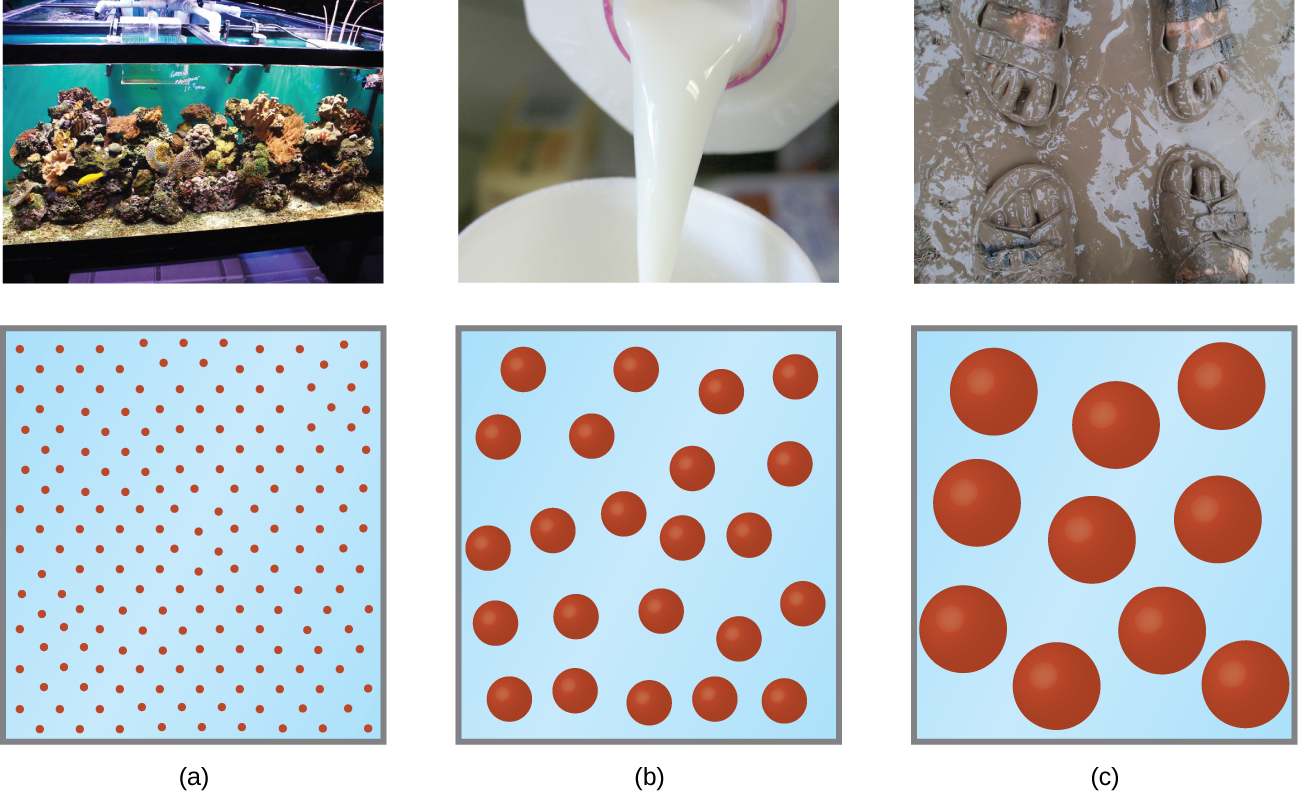
\includegraphics[scale=0.8]{figures/Colloid.png}
\caption[Dissolucions, suspensions i col·loides]{(a) Una dissolució és una mescla homogènia, com l'aigua salada de l'aquari. (b) En un col·loide les partícules són més grans, però es mantenen disperses i no precipiten (llet). (c) Una suspensió és una mescla heterogènia amb particules que poden acabar precipitant. (adaptat de \cite{Colloids2016})}
\label{fig:Colloid}
\end{figure}

\begin{table}[h!]
  \begin{center}
    \caption{Diferents tipus de dispersions}
    \label{tab:colloid}
    \begin{tabular}{l|l|l|l}
      & \multicolumn{3}{c}{Dispersant}\\ 
      \hline
      Dispers & Sòlid & Líquid & Gas\\
      \hline
      Sòlid & Alguns al·liatges; gemmes acolorides & Gels o suspensions (pintures) & Aerosols (fum) \\
      Líquid & Geles (gelatina) & Emulsions & Aerosols (boira) \\
      Gas & Escuma aïllant & Escuma (cervesa) & \\
      \hline
    \end{tabular}
  \end{center}
\end{table}
\item La \emph{matèria homogènia} és aquella que és idèntica quant a composició i propietats sigui quina sigui la porció que n'agafem. L'aigua de mar, la sal o un lingot d'or en són exemples:
\begin{itemize}
\item L'aigua de mar és una \emph{dissolució}, en tant que formada per dos o més components. Les propietats d'una dissolució poden ser radicalment diferents de les dels seus components: aigua i sal no són conductors de l'electricitat, però la seva dissolució ho és. Les dissolucions són homogènies a la subdivisió, però heterogènies al canvi d'estat. Els components no es poden barrejar en qualsevol proporció (per exemple, la solubilitat depèn de la temperatura). Les propietats depenen de la concentració, com mostra la Figura \ref{fig:watsuc2} (temperatura d'ebullició o fusió de l'aigua amb sals o anticongelants).
\begin{figure}[h]
\centering
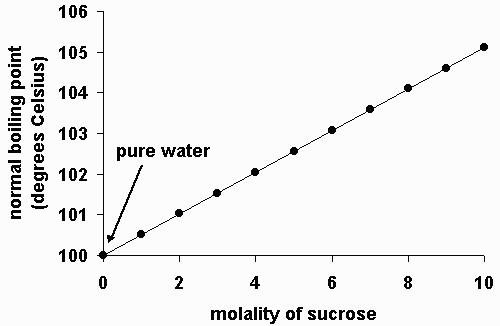
\includegraphics[scale=0.8]{figures/watsuc2.png}
\caption{La temperatura d'ebullició d'una dissolució aquosa es modifica en funció de la concentració de solut.}
\label{fig:watsuc2}
\end{figure}
\item La sal i l'or són \emph{substàncies pures}, en tant que formades per un sol component i amb propietats físiques i químiques característiques d'aquests (densitat, temperatura de fusió o d'ebullició, solbilitat en un dissolvent donat, índex de refracció, viscositat, etc).
\end{itemize}
\end{itemize}


La Figura \ref{fig:SeparacioMescles} mostra un resum esquemàtic dels processos per reduir la complexitat d'una determinada mescla.

\begin{figure}[h]
\centering
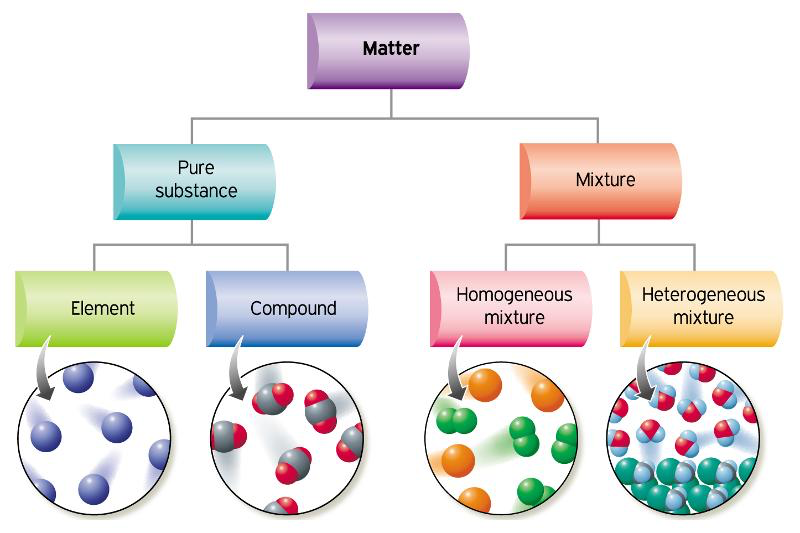
\includegraphics[scale=0.35]{figures/Mixtures.png}
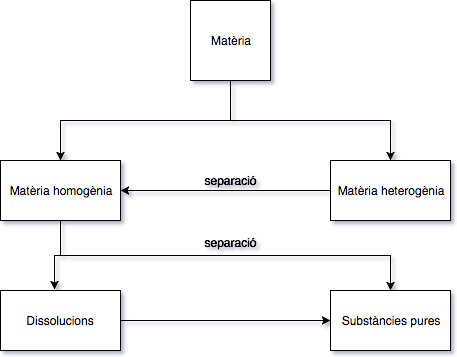
\includegraphics[scale=0.50]{figures/SeparacioMescles.png}
\caption{Classificació de la matèria (adaptat de \cite{Caamano1984})}
\label{fig:SeparacioMescles}
\end{figure}

Algunes tècniques de separació:
\begin{itemize}
\item mètodes simples de separació de mescles: filtració, decantació, centrifugació, cristal·lització, destilació, etc;
\item mètodes per separar mescles de múltiples components: 
\begin{itemize}
\item cristal·lització fraccionada (dos sòlids amb solubilitats diferents);
\item destil·lació fraccionada (dos líquids de punts d'ebullició semblants amb columnes de fraccionament, veure Figura \ref{fig:Crude_Oil_Distillation_Unit});
\item cromatografia (d'adsorció, de repartiment, d'intercanvi iònic, de filtració sobre gels); sobre paper, de columna, sobre capa fina...; gas-sòlid, líquid-líquid, gas-líquid.
\end{itemize}  
\begin{figure}[h]
\centering
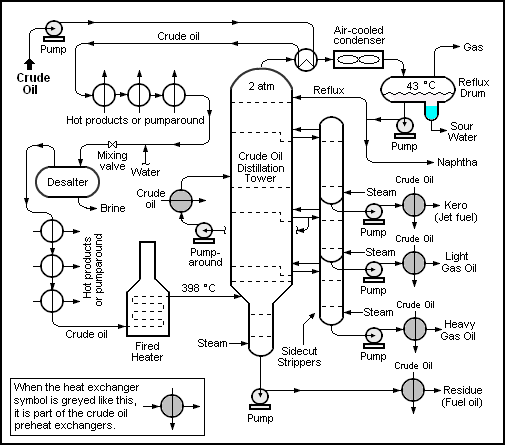
\includegraphics[scale=0.8]{figures/Crude_Oil_Distillation_Unit.png}
\caption{Esquema de la columna de destilació del petroli.}
\label{fig:Crude_Oil_Distillation_Unit}
\end{figure}
\end{itemize}

Per a caracteritzar la puresa d'una substància, analitzem les seves propietats característiques mitjançant tècniques molt diverses, entre elles l'anàlisi dels seus espectres:
\begin{itemize}
\item espectroscopia infraroja (IR), 
\item espectroscopia visible i ultraviolada (UV)
\item espectroscopia de resonància magnpetica nuclear (NMR)
\item difracció de raigs X
\item espectroscopia de masses
\item etc
\end{itemize}

\subsection{Elements i compostos}

Els \emph{compostos} es poden descomposar en substàncies més simples. En canvi, els \emph{elements} o substàncies simples són indivisibles. Addicionalment, un compost es pot sintetitzar a partir de substàncies més simples, cosa que no passa amb els elements (Figura \ref{fig:CompostosElements}). 

Robert Boyle va donar la primera definició d'Element l'any 1661. Lavoisier va donar una llista d'elements coneguts el 1789 però hi va incloure la llum i la calor. També va formular la llei de la conservació de la massa. El 19800, Alessandro Volta va inventar la pila elèctrica i va permetre separar nous elements (electròlits) per part de Humphry Davy el 1807: el sodi i el potassi. El mateix 1807, Dalton publica la seva teoria atòmica.

Es poden combinar els elements de qualsevol manera per formar compostos? Ho veurem a la secció següent.

\begin{figure}[h]
\centering
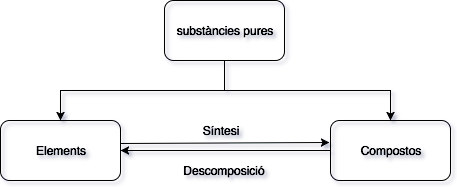
\includegraphics[scale=0.8]{figures/CompostosElements.png}
\caption{Relació entre compostos i elements.}
\label{fig:CompostosElements}
\end{figure}


\section{La naturalesa atòmica de la matèria}

Durant molts anys l'observació de fenòmens químics senzills va servir per determinar les lleis fonamentals de la química que la van distingir de l'alquímia.

\begin{mdframed}[backgroundcolor=gray!30,frametitle=Llei de les proporcions definides]
En un compost donat, els elements constituients es combinen sempre en les mateixes proporcions pondarebles, sigui quin sigui l'origen i el mode de preparació dels compostos.
\end{mdframed}

Veurem que a cada element se li pot assignar un pes determinat i això fa que la seva combinació dongui un pes determinat i una fórmula determinada als compostos.
Per exemple, si pensem en l'òxid nítric, \ch{NO} i mirem d'augmentar el mínim possible (un àtom d'oxigen o un de nitrogen) arribem a nous compostos molt diferents de l'inicial i entre ells, \ch{N2O} i \ch{NO2}. 

De fet, la llei és força simple i poc precisa, ja que els elements poden tenir diferents isòtops.
Els isòtops d'un element tenen diferents masses atòmiques (sempre tindran el mateix número de protons, però poden diferir en el número de neutrons). La massa atòmica promig es mesura ponderant les masses atòmiques de cada isòtop amb la seva abundància a la terra (veure Figura \ref{fig:PropietatsHidrogen}).
Els objectes extraterrestres poden tenir composicions isotòpiques molt diferents.
\begin{figure}[h]
\centering
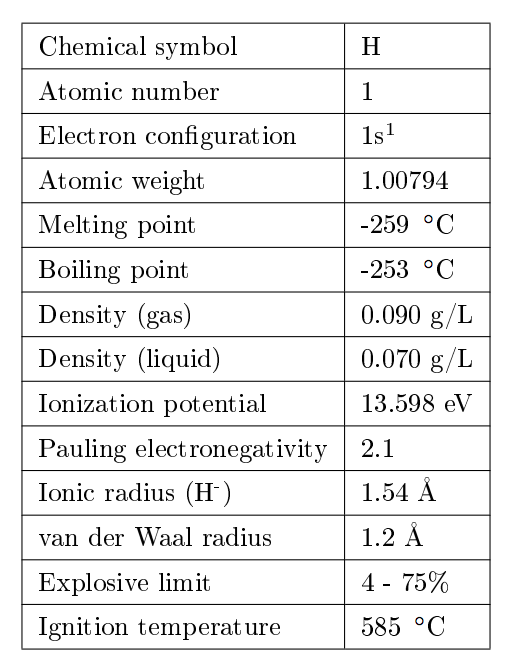
\includegraphics[scale=0.35]{figures/PropietatsHidrogen.png}
\caption{Propietats físiques de l'àtom d'hidrogen (Adaptat de Connexions \linkurl{http://cnx.org/content/col10984/1.4})}
\label{fig:PropietatsHidrogen}
\end{figure}
\begin{exr}
Entra a \linkurl{https://teachchemistry.org/periodical/issues/may-2017/isotopes-calculating-average-atomic-mass} i calcula la massa atòmica promig d'alguns elements.
\end{exr}
També es viola aquesta llei en alguns sòlids iònics com l'òxid de zinc, el sulfur cuprós (entre \ch{Cu_{1.7}S} i \ch{Cu2S}) o l'òxid ferrós.

Els compostos sòlids que no estan formats per molècules definides presenten característiques diferents. Podem preparar cristalls de \ch{TiO}, però variant les condicions de preparació podem anar de \ch{Ti_{0.75}O} a \ch{TiO_{0.69}}, encara que la seva estructura espaial sigui idèntica. Es tracta de compostos no estequiomètrics i, tot i que no varïin les seves propietats estrcuturals, sí que ho fan les òptiques o la resistivitat (veure Figura \ref{fig:TiOPhaseDiagram}).
\begin{figure}[h]
\centering
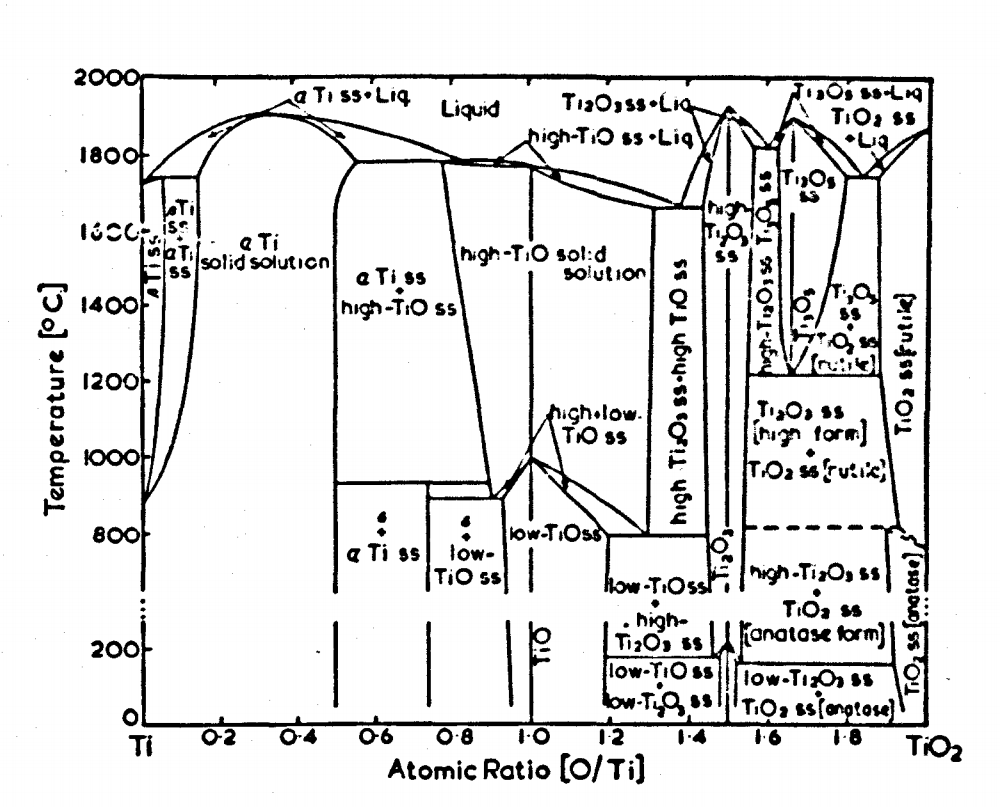
\includegraphics[scale=0.35]{figures/TiOPhaseDiagram.png}
\caption{Diagrama de fase de l'òxid de titani en diverses composicions (no)estequiomètriques\cite{DeVries1954}}
\label{fig:TiOPhaseDiagram}
\end{figure}

\begin{mdframed}[backgroundcolor=gray!30,frametitle=Llei de les proporcions múltiples]
Si dos elements formen més d'un compost, els diferents pesos d'un d'ells que es combinen amb el mateix pes de l'altre, estan en una relació de números enters petits.
\end{mdframed}

Els diferents òxids del nitrogen en són un bon exemple: amb 16g d'oxigen es poden combinar 28, 14 o 7 grams de nitrogen (proporció 4:2:1)

\begin{mdframed}[backgroundcolor=gray!30,frametitle=Llei de les proporcions equivalents]
Si una determinada quantitat de l'element C reacciona amb una quantitat donada de l'element A, p$_A$, i una donada de l'element B, p$_B$, A i B reaccionen en una proporció que és múltiple simple o fracció de números sencers de la raó p$_A$/p$_B$.
\end{mdframed}

El nitrogen i l'oxigen reaccionen amb l'hidrogen per formar amoniac (\ch{NH3}) i aigua (\ch{H2O}), respectivament. 1g d'hidrogen reacciona amb 4,66g de Nitrògen per formar amoniac i amb 8 grams d'oxigen per formar aigua. Per tant, 4.66/8.00=0.583.
En el cas de la reacció \ch{N2 + O2 -> 2NO}, 28g de nitrogen reaccionen amb 32g d'oxigen. 28/32=0.875, que és 1.5 vegades 0.583 o, el que és el mateix, la fracció 3/2.



\subsection{Pesos atòmics i fòrmules moleculars (M)}

En principi, doncs, era possible relacionar els pesos de tots els elements i la manera en què es combinaven. El problema és que no es tenia cap certesa sobre cap compost inicial, ni sobre cap pes atòmic. Dalton no podia fer més que conjectures.

Gay-Lussac va mostrar el volum de la combinació de dues substàncies estava relacionat amb números sencers, com també marcava la llei de proporcions múltiples. Entre aquesta observació i l'admissió de que els elements nitrogen i oxigen podien ser poliatòmics, va dur Amedeo Avogadro (1811) es van acostar a la determinació dels pesos moleculars, però encara hi havia indeterminació. Finalment, Cannizaro va crear l'escala de pesos a partir de l'observació que la teoria atòmica de Dalton establia que el níumero d'àtoms en una molècula havia de seguir proporcions senceres. Va establir el pes de l'hidrogen com a 2g.

Per ser més precisos en la determinació de pesos atòmics es poden usar altres tècniques. Per exemple, considerant que a temperatura 0K els gasos es comporten de manera ideal i la densitat és proporcional a la pressió ($\delta=\alpha P$, on $\alpha$ seria la densitat que tindria un gas ideal a pressió 1 atm) però que a pressions més elevades cal millorar aquesta aproximació ($\delta = \alpha P + \beta P^2$), podem graficar $\delta/P$ en funció de la $P$ i obtindrem línies rectes com la de la Figura \ref{fig:DensitatIdealCO2}.
\begin{figure}[h]
\centering
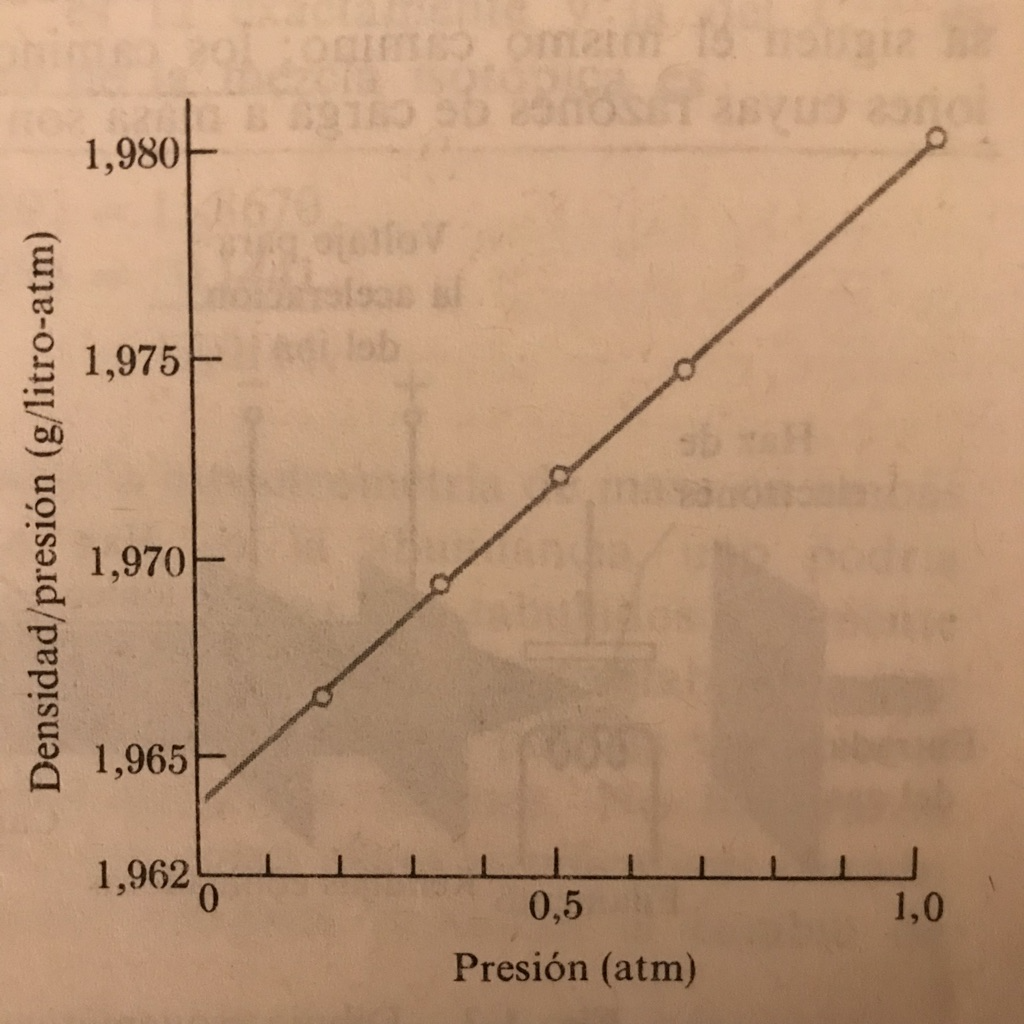
\includegraphics[scale=0.3]{figures/DensitatIdealCO2.png}
\caption{Determinació de la densitat ideal del \ch{CO2} a 273,1$^º$K.}
\label{fig:DensitatIdealCO2}
\end{figure}
\begin{exr}
Si la densitat del gas oxigen és de 1.428g/l a 1atm i 273.1K i la del \ch{CO2} és 1.9635g/l a les mateixes condicions, i si el pes molecular de l'oxigen és 31,998, quin és el pes molecular del \ch{CO2}?
\end{exr}

\begin{mdframed}[backgroundcolor=gray!30,frametitle=Concepte de mol]
El número d'àtoms de carboni contingut en, exactament, 12g de \ch{C^{12}} s'anomena número d'Avogadro, \emph{N}. Un mol és la quantitat de matèria que conté el número d'Avogadro de partícules.
\end{mdframed}

\newpage

\subsection{Estequiometria (M)}

\section{Gasos}
\label{sec:gasos}

Dels gasos podem mesurar una sèrie de propietats característiques que ens permeten el seu estudi precís: \textbf{massa}, \textbf{volum}, densitat, \textbf{pressió}, \textbf{temperatura}, compressibilitat, coeficient de dilatació tèrmica, capacitat calorífica, viscositat, conductivitat tèrmica, difusivitat, etc, de les quals hem remarcat les anomenades \textbf{propietats primàries}.

La pressió es mesura en el S.I. en Pascals:
\[
1 {\rm Pa}=\frac{1 {\rm N}}{1 {\rm m}^2}
\]
però es treballa sovint en atmosferes (1 atm = 1.01325 $\times$ 10$^5$ Pa = 760 Torr = 760 mmHg).
\begin{figure}[h]
\centering
\includegraphics[scale=0.33]{figures/Manometre.png}
\caption[Manòmetre diferencial]{Un manòmetre diferencial mesura la diferència entre les pressions externes i d'un determinat gas. Cal tenir en compte la pressió atmosfèrica exterior (approx 1 atm).}
\label{fig:Manometre}
\end{figure}
Les equacions que depenen de les quatre propietats primàries s'anomenen equacions d'estat:
\[F(p,m,V,T)=0\]
En situacions normals (absència de camps elèctrics externs, per exemple) tres de les propietats són suficients per determinar la quarta (10g de N$_2$ a 30$\degree$C no podem saber en quin estat es troben -spolid, líquid o gas- ja que ens manca conèixer la pressió, i així en qualsevol situació).

D'altra banda, les propietats es poden classificar entre extensives (m, V, ...) o intensives (T, P, capacitat calorífica ...), segons depenguin de la quantitat de substància o no. La raó entre dues propietats extensives és sempre intensiva: $\delta = \frac{m}{V}$; $\nu = \frac{V}{m}$. Només necessitem dues propietats intensives per determinar l'estat d'un gas ($P$ i $T$) i, per tant, amb tres variables intensives podem construir una equació d'estat: 
\[F(p,V_{\rm m},T)=0\]

La mesura d'una propietat per mol sanomena valor molar d'aquesta variable: $V_{\rm m} = \frac{V}{n}$. 
\subsection{Llei de Boyle}

Robert Boyle (1627-1691) va notar, fent servir un manometre com el de la Figura \ref{fig:Manometre}, que existia una determinada llei de proporcionalitat entre la pressió exercida sobre un gas i el volum d'aquest
\begin{figure}[h]
\centering
\includegraphics[scale=0.10]{figures/Boyle.png}
\caption{Experiment de Boyle i llei de proporcionalitat entre la pressió exercida sobre un gas i el seu volum.}
\label{fig:Boyle}
\end{figure}
Va descobrir que el producte entre el volum i la pressió és una constant, la qual cosa duu a que sota dues condicions diferents de pressió els volums es comporten de la següent manera per al mateix gas a una temperatura donada:
\[
\frac{V_1}{V_2}=\frac{P_2}{P_1}
\]


\subsection{Llei de Charles i Gay-Lussac}

JAcques Charles (1787) i posteriorment Gay-Lussac van trobar que per a una mateixa pressió, la relació $\frac{V_{100 \degree C}}{V_{0 \degree C}}$ era identica per a tots els gasos (1.376).

Això duu a extrapolar fàcilment el comportament dels gasos i determinar el zero absolut de temperatura segons el gràfic \ref{fig:zeroabsolut}. Lord Kelvin (1848) va proposar usar el punt d'intersecció del gràfic amb la línia de les abcisses com a origen d'una nova escala de temperatura: $T/\rm{K} = t/\degree \rm{C} + 273.15$.\footnote{en realitat s'usa 273.16, que és el punt triple de l'aigua, temperatura a la qual coexisteixen en equilibri aigua, gel i vapor en un recipient tancat}
\begin{figure}[h]
\centering
\includegraphics[scale=1.0]{figures/zeroabsolut.png}
\caption{Gràfic del zero absolut a partir de la llei de Charles i Gay-Lussac.}
\label{fig:zeroabsolut}
\end{figure}

De la nova llei es desprèn que 
\[\frac{P V_{\rm m}}{T}= cnt = R\]
o bé
\[P V = n R T\]
que es coneix com a equació d'estat d'un gas ideal.

\subsection{Gas ideal}

Per tal de determinar la $R$ no podem simplement calcular el quocient $\frac{P V_{\rm m}}{T}$ per a qualsevol gas, ja que cadascun d'ells donarà un valor diferent (només és vàlida l'expressió per a un gas ideal!). Veure la Figura \ref{fig:R2}.
\begin{figure}[h]
\centering
\includegraphics[scale=1.0]{figures/R2.png}
\caption[Determinació de la constant dels gasos $R$]{R es pren com al valor límit de la fracció $\frac{P V_m}{T}$ per a tots els gasos: 
$R=\lim_{P \to 0} \frac{P V_{\rm m}}{T}= 0.08205 \frac{{\rm atm l}}{{\rm mol K}}$
}
\label{fig:R2}
\end{figure}

\begin{exr}
Calcular el volum molar d'un gas ideal a condicions normals (1 atm i 0$\degree$C).
\end{exr}

\begin{exr}
Quant gas hi ha en una mostra de volum 0.5 dm$^3$, a 80 graus Celsius i 800 Torr de pressió?.
\end{exr}

\begin{exr}
Un conductor comprova la pressió dels pneumàtics pel matí aviat, quan la temperatura és de 15$\degree$C, i és de 1.3$\times$10$^5$ Pa. Al migdia la temperatura és 15 graus més elevada. Quina és la pressió dels pneumàtics ara?.
\end{exr}

\begin{exr}
Si a CN la densitat d'un gas ideal és de 1.62 g dm$^{-1}$, quina és la seva massa molar? i quina densitat tindrà a 300 K i 2.4$\times$10$^5$ Pa?.
\end{exr}

\begin{exr}
Dalt de l'Everest, la pressió atmosfèrica és de 0,33 atm i la temperatura de 50 sota zero. Quina és la densitat de l'aire i en CN és de 1.29 g dm$^-3$?.
\end{exr}

\subsection{Teoria cinètica dels gasos (M)}

Per tal de relacionar aquestes descobertes amb l'estructura atòmica de la matèria, ens cal pensar una teoria que representi els gasos de forma extremadament simple: un \textit{model}. En el nostre cas (veure Figura \ref{fig:TeoriaCinetica}),
\begin{itemize}
\item el gas es format per partícules que es comporten com a punts de massa,
\item que llevat no col·lideixin no exerceixen força els uns sobre els altres
\end{itemize}
\begin{figure}[h]
\centering
\includegraphics[scale=0.2]{figures/TeoriaCinetica.png}
\caption{Representació del moviment de les partícules en un gas ideal.}
\label{fig:TeoriaCinetica}
\end{figure}
\begin{exr}
Pots calcular el volum ocupat per molècula en un gas ideal a CN?. Es troben dues molècules molt freqüentment en un gas a baixa pressió?
\end{exr}
Aquesta teoria, de forma relativament simple, ens permet expressar la pressió que s'exercexi sobre les parets d'un recipient per part del gas que conté segons:
\[
PV=\frac{2}{3} \left< E_c \right> = \frac{2}{3} \left< \frac{mc^2}{2} \right>
\]

D'aquí s'extreuen resultats interessants, com que l'energia cinètica translacional d'un mol de gas és \[N_0 \frac{m <c^2>}{2}=\frac{3}{2} RT\] o bé, si dividim pel número d'Avogadro a esquerra i dreta obtenim la constant dels gasos per molècula a partir de l'energia cinètica per molècula (constant de Boltzmann $k$): \[\frac{m <c^2>}{2}=\frac{3}{2} kT\].
Aquest resultat ens diu que si dos gasos tenen la mateixa $T$, les seves molècules tenen la mateixa energia cinètica promig. 
\begin{exr}
Qui es mou més ràpid, una molècula d'oxigen o una de nitrogen en dues mostres d'aquests gasos a la mateixa temperatura? Pots explicar perquè la pressió és independent de la natura de les molècules?
\end{exr}

\begin{exr}
Calcula la velocitat mitjana de les molècules d'hidrògen a 25$\degree$C.
\end{exr}

La distribució de les velocitats de les partícules d'un gas segueix la distribució de Maxwell-Boltzmann:
\[
\frac{\Delta N}{N}=4 \pi \left( \frac{m}{2 \pi kT}\right)^{3/2} \underbrace{e^{-mc^2/2kT}}_{\rm Boltzmann} c^2 \Delta c
\]
El factor de Boltzmann ens diu, en aquesta equació, que a qualsevol temperatura particular, acostuma a haver moltes menys molècules amb energies altes que amb energies baixes.
\begin{figure}[h]
\centering
\includegraphics[scale=0.5]{figures/BolzDist.png}
\includegraphics[scale=0.5]{figures/MXDIST.png}
\caption{La distribució de Maxwell per a diferents molècules i temperatures}
\label{fig:TeoriaCinetica}
\end{figure}

\subsection{Capacitat calorífica}

La capacitat calorífica d'una substància és la quantitat de calor en calories necessària per elevar 1$\degree$C la temperatura d'un gram de la substància.

De fet, això necessita precissió: no és el mateix fer aquest procés dpescalfament a volum constant que a pressió constant ($C_V$ vs $C_P$).

Si afegim calor a un gas, o bé s'expandeix (i per tant fa treball) o bé la velocitat de les seves particules augmenta.
A $V$ constant, l'escalfament produeix un increment d'energia cinètica:
\[\Delta E = \frac{3}{2} R \Delta T\]
però resulta que $\Delta E/ \Delta T$ és, justament, $C_V$ i, per tant, per a un gas monoatòmic ideal, $C_V=\frac{3}{2}R$ o, aproximadament, 3 cal/mol·grau.

En el cas de pressió constant, les partícules augmenten la seva energia cinètica i també exerceixen treball ($\Delta(PV)$):
\[\Delta(PV)=P\Delta V = P(V_2-V_1)=PV_2-PV_1\]
Per a un mol de gas, resulta que $PV=RT$ i, per tant, 
\[PV_2-PV_1=RT_2-RT_1=R\Delta T\]
Per tant, la capacitat calorífica extra pel fet de fer el procés a pressió constant és
\[\frac{\Delta (PV)}{\Delta T}=R\]
i, per tant, 
\[C_P=C_V+R \\
=\frac{3}{2} R + R= \frac{5}{2}R\]
És fàcil veure que $C_P/C_V=5/3=1.67$ i podem comparar aquests coeficients per a diversos gasos reals, per tal d'establir diferències amb el seu comportament ideal (\ref{tab:cpcv}).
\begin{table}[h!]
  \begin{center}
    \caption{Quocients de capacitat calorífica \cite{Mahan1977}}
    \label{tab:cpcv}
    \begin{tabular}{cc|cc}
      \hline
      Gas & $C_P/C_V$ & Gas & $C_P/C_V$\\
      \hline
      He & 1.66 & \ch{H2} & 1.41 \\
      Ne & 1.66 & \ch{O2} & 1.40 \\
      Ar & 1.66 & \ch{N2} & 1.40 \\
      Kr & 1.66 & \ch{CO} & 1.40 \\
      Xe & 1.66 & \ch{NO} & 1.40 \\
      Hg & 1.66 & \ch{Cl2} & 1.36 \\
      \hline
    \end{tabular}
  \end{center}
\end{table}
\begin{exr}
Perquè hi ha aquestes diferències entre la columna de l'esquerra i la de la dreta de la Taula \ref{tab:cpcv}? (Adona't que si un gas monoatpomic ideal, pel fet d'estar només augmentant la seva energia cinètica té una $C_V=\frac{3}{2}R$, es pot entendre que per a cada component necessita $\frac{3}{2}R$)
\end{exr}




\subsection{Gasos no ideals}

En gasos reals, el factor 
\[z=\frac{V_m}{V_{m,i}}=\frac{V_m}{RT/P}=\frac{PV_m}{RT}\]
no és 1, com succeiria a un gas ideal (veure Figura \ref{fig:FactorCompress}).
\begin{figure}[h]
\centering
\includegraphics[scale=0.5]{figures/FactorCompress.png}
\caption{Factor de compressibilitat per a diferents gasos a 0$\degree$C}
\label{fig:FactorCompress}
\end{figure}

Per tal de millorar l'aproximació a la realitat podem considerar diferents aproximacions. La més simple consisteix a pensar que el volum ideal explorat per les molècules és més gran que el volum que poden explorar en realitat, per un valor $b$ que prové del volum exclós per la presència d'altres molècules.
\[V_m = V_{m,i}+b=\frac{RT}{P}+b\]

Segons això,
\[z=\frac{PV_m}{RT}=1+\frac{b}{RT}P\]
que té una forma lineal. Aixó explicaria el cas de la molècula d'hidrogen.
Però què passa amb \ch{CH4} o \ch{CO}? Val la pena pensar que són molècules que es podran trobar líquides a temperatures més baixes amb major facilitat que no pas \ch{H2}. En un gas real, la pressió que exerciran les molècules sobre la paret del recipient serà més baixa que en un gas ideal:
\[P=P_i -\Delta P\]
Es pot veure que aquest increment de pressió és proporcional al quadrat de la concentració ($c=\frac{m}{V}=\frac{1}{V_m}$):
\[\Delta P \alpha c^2 \alpha \frac{1}{{V_m}^2} \]
o bé
\[\Delta P = \frac{a}{{V_m}^2}\]
i, per tant, 
\[ P_i=P+\frac{a}{{V_m}^2}\]

Si ara substituïm el volum i pressió ideals en l'equació dels gasos ideals:
\[
\left( P + \frac{a}{{V_m}^2} \right) (V_m -b)=RT
\]
o bé
\begin{equation}
\left( P + \frac{n^2 a}{V^2} \right) (V -nb)=nRT
\label{Eq:vdW}
\end{equation}

\begin{exr}
Què passa segons l'Equació \ref{Eq:vdW} si la pressió es fa propera a zero o bé la temperatura es fa molt gran per a un gas real? (veure la Figura \ref{fig:FactorCompressT}).
\end{exr}

\begin{figure}[h]
\centering
\includegraphics[scale=1.0]{figures/FactorCompressT.png}
\caption{Factor de compressibilitat per a un mateix gas a diferents temperatures}
\label{fig:FactorCompressT}
\end{figure}

Les forces de van der Waals que fan que es perdi la idealitat són degudes a tres contribucions:
\begin{enumerate}
\item Efecte d'orientació: forces dipol-dipol.
\item Efecte de distorsió: forces d'inducció.
\item Efecte de dispersió: forces de dispersió.
\end{enumerate}

\begin{exr}
Perquè \ch{CO2} i \ch{O2} tenen una desviació negativa respecte al comportament del gas ideal a pressions i temperatures moderades, mentres que l'He i el \ch{H2} presenten una deviació positiva en les mateixes condicions?
\end{exr}


%\subsection{Fenòmens de transport (M)}



\section{Sòlids}
\subsection{Propietats (M)}

Es caracteritzen per la seva rigidesa, incompressibilitat i per les seves característiques geomètriques.
La teoria atòmica ens ajuda a entendre el seu comportament basat en l'estructura d'una xarxa cristalogràfica.



\subsection{Tipus (M)}

Podem distingir:
\begin{description}
\item[sòlids cristal·lins] Exemples: clorur sòdic, sofre... 
\begin{itemize}
\item Són anisotròpics (la refracció, la conductivitat elèctrica, etc, depenen de la direcció en la qual es mesurin). 
\item Tenen punts de fusió ben definits. 
\item Es presenten a la natura sota formes polièdriques limitades per cares planes.
\end{itemize}
\item[substàncies amorfes] Exemples: vidre, plàstic... \begin{itemize}
\item No tenen caracterìstiques regulars. 
\item Són isotròpics. 
\item No estan ben establerts (són progressius) els seus punts de fusió.
\end{itemize}
\end{description}
Tots dos tipus de substàncies tenen alguna mena d'interacció local d'enllaç, però en el cas dels sòlids amorfs no existeix cap cel·la unitat.

La formació dels cristalls és depenent de la temperatura i la velocitat del procés en què es formen. Processos lents impliquen cristalls més grans, per exemple.

Els cristalls es poden estudiar per difracció de raigs X, que es basa en el fet que la longitud d'ona dels raigs X és similar a l'espaiat dels àtoms en el cristall. 

\begin{table}[h!]
  \begin{center}
    \caption[Sistemes cristal·lins i retícules de Bravais]{Sistemes cristal·lins i retícules de Bravais (veure Figura \ref{fig:Bravais}). P: centrada en les cantonades; I: centrada en el cos; F: centrada en la cara; C: amb punt central (adaptat de \cite{Yen2008}).}
    \label{tab:Bravais}
    \begin{tabular}{cccc}
      \hline
      Sistema & Cel·la unitat & retícula de Bravais \\ 
      \hline
	  Cúbic      & $a=b=c$ & P,I (Fig. \ref{fig:crystal_structure}b),F (Fig. \ref{fig:crystal_structure}a)\\
	             & $\alpha=\beta=\gamma=90\degree$ & \\
	  Tetragonal & $a=b\neq c$ & P,I \\
	             & $\alpha=\beta=\gamma=90\degree$ & \\
	  Ortoròmbic & $a\neq b\neq c$ & P,I,C,F\\
	             & $\alpha=\beta=\gamma=90\degree$ & \\
	  Romboèdric & $a=b=c$ & R(P)\\
	             & $\alpha=\beta=\gamma \neq 90\degree$ & \\
	  Hexagonal  & $a=b\neq c$ & P (Fig. \ref{fig:crystal_structure}c) \\
	             & $a=b \neq c$ & \\
	             & $\alpha = \beta = 90 \degree$ & \\
	             & $\gamma = 120\degree$ &\\
	  Monoclínic & $a \neq b \neq c$ & P,C\\
	             & $\alpha=\gamma \neq \beta$&\\
	  Triclínic  & $a \neq b \neq c$ & P\\
	             & $\alpha \neq \beta \neq \gamma$&\\
      \hline
    \end{tabular}
  \end{center}
\end{table}


\begin{figure}[h]
\centering
\includegraphics[scale=0.1]{figures/Bravais.png}
\caption{Retícules de Bravais i relació amb els 7 típus de cel·la unitat \cite{Yen2008}.}
\label{fig:Bravais}
\end{figure}
\begin{figure}[h]
\centering
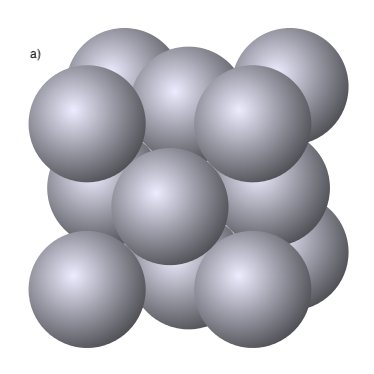
\includegraphics[scale=0.4]{figures/FCC_crystal_structure.png}
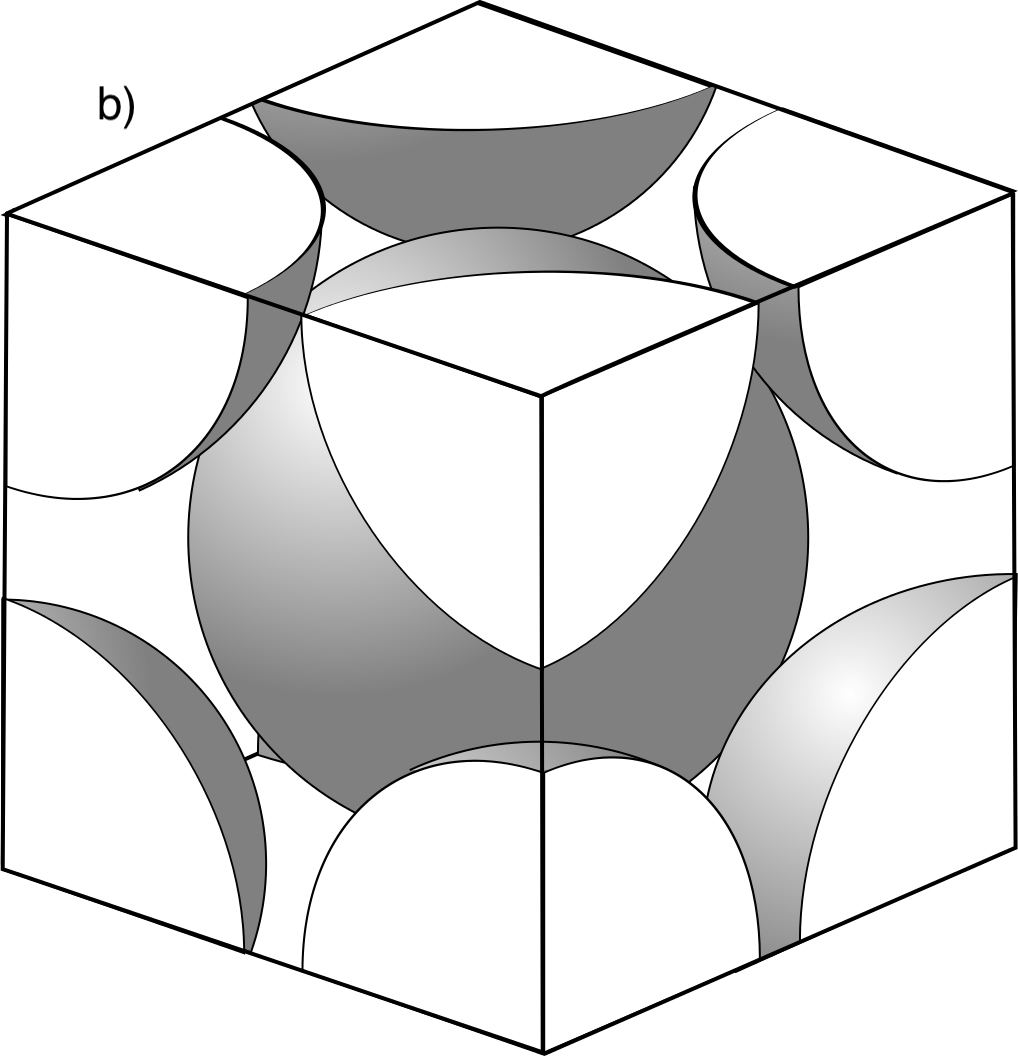
\includegraphics[scale=0.12]{figures/CBC_crystal_structure.png}
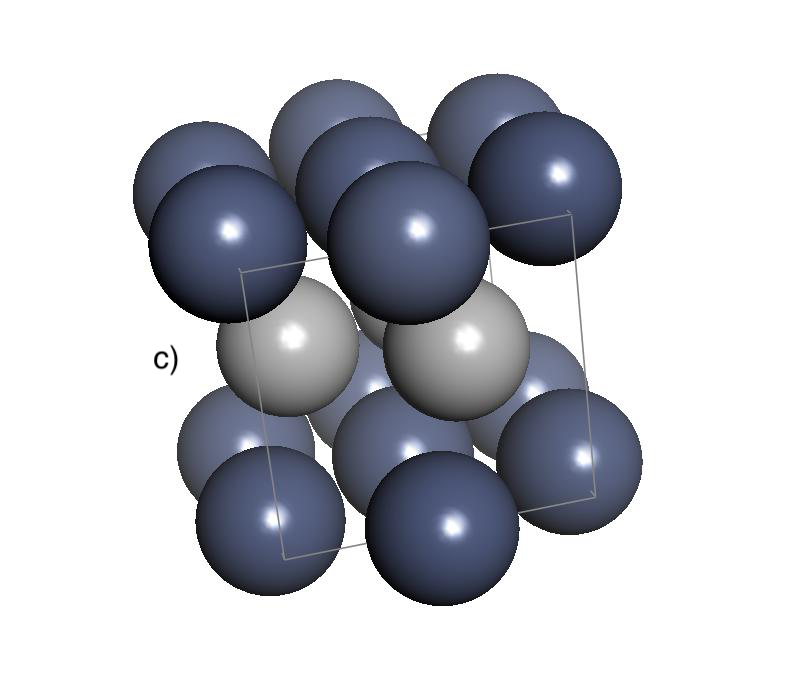
\includegraphics[scale=0.32]{figures/HCP_crystal_structure.png}
\caption[Exemples d'estructures cristal·lines]{Exemples d'estructures: a) cel·la unitat cúbica centrada en la cara, amb 4 àtoms per cel·la unitat; b) cel·la unitat cúbica centrada en el cos; c) hexagonal (en la imatge, Hidrur de Crom, \ch{CrH_x})}
\label{fig:crystal_structure}
\end{figure}

\begin{exr}
La ratio d'empaquetament d'una cel·la unitat es defineix com la fracció entre el volum omplert pels àtoms que la formen i el seu volum total. Calcula el RE de la cel·la unitat cúbica centrada en la cara i de la cel·la unitat cúbica centrada en el cos (veure Figura \ref{fig:crystal_structure}).
\end{exr}

La Figura \ref{fig:bonding_motifs_PT} mostra els modes d'empaquetament dels elements de la taula periódica. A partir dels modes d'empaquetament també es poden calcular relacions diverses que ens indiquen el grau de direccionalitat dels enllaços entre els diferents àtoms, ajudant a identificar els diferents tipus de sòlids cristal·lins.
\begin{figure}[h]
\centering
\includegraphics[scale=0.13]{figures/bonding_motifs_PT.png}
\caption{Estructura cristal·lina o modes d'enllaç a la taula periòdica \cite{Yen2008}.}
\label{fig:bonding_motifs_PT}
\end{figure}

Podem distingir cinc tipus de sòlids, com es veu a la Taula \ref{tab:TipusSolids}.\footnote{veure també \linkurl{https://chemistry.tutorvista.com/inorganic-chemistry/types-of-solids.html}}
\begin{table}[h!]
  \begin{center}
    \caption{Tipus de sòlids (adaptat de \cite{Yen2008}.}
    \label{tab:TipusSolids}
    \begin{tabular}{llllr}
      \hline
      Tipus & Components & característiques & Exemples & Energia de cohesió \\ 
            &         &                  &          & (kJ mol$^{-1}$) \\ 
      \hline
Iònic   &  càrregues $+$ i $-$ & fràgils, aïllants             & NaCl     & 795 \\
        &                      & alt punt de fusió             & LiF      & 1010 \\
Covalent&  àtoms enllaçats     & durs, no conductors (si purs),& diamant  &   715 \\
        &                      & alt punt de fusió             & SiC      & 1010  \\
Metàl·lic & ions positius en     &  molt conductors            & Na       & 110  \\
          & un núvol d'electrons &                             & Fe       & 395  \\
vdW (mol·leculars) &  molècules o àtoms &  tous, baix punt de fusió,  &  Ar   &  7.6  \\
                   &                    & volàtils i aïllants         &  \ch{CH4} &  10  \\
Enllaç d'hidrogen  &  molècules amb enllaços  & baixa fussió, aïllants & \ch{H2O} &  50  \\
                   &  d'hidrogen              &                        & \ch{HF}  &  30  \\
      \hline
    \end{tabular}
  \end{center}
\end{table}

\subsubsection{Cristalls metàl·lics}
  
Per entendre l'estructura dels metalls, considerem primer que els nuclis d'un determinat element són formant un cristall de les característiques que hem explicat més amunt i que es representen a la Figura \ref{fig:bonding_motifs_PT}. Els elements metàlics tenen energies d'ionització baixes (de menys de 220 kcal mol$^{-1}$, exccepte en el cas del mercuri, on és de 240 kcal mol$^{-1}$), amb la qual cosa tenen tendència a perdre amb facilitat els electrons més externs (anomenats de valència; veurem més endavant com podem racionalitzar això). Per tant, aquests electrons estan poc atrets i, per tant, formaran enllaços covalents poc forts, com es veu a la Taula \ref{tab:DisMet}. 
Serà més forta la interacció dels electrons de valència amb molts àtoms que no pas amb només dos.
\begin{table}[h!]
  \begin{center}
    \caption{Energies de dissociació de molècules d'elements metàlics en kcal mol$^{-1}$ (adaptat de \cite{Mahan1977}.)}
    \label{tab:DisMet}
    \begin{tabular}{llll}
      \hline
\ch{Li2} & 25 & \ch{Zn2} & 5.7 \\
\ch{Na2} & 17 & \ch{Cd2} & 2.0 \\
\ch{K2}  & 12 & \ch{Hg2} & 1.4 \\
\ch{Rb2} & 11 & \ch{Pb2} & 16 \\
\ch{Cs2} & 10.4 & \ch{Bi2} & 39 \\
\ch{NaK} & 14 & \ch{NaRb} & 13\\
      \hline
    \end{tabular}
  \end{center}
\end{table}

També veurem que el seu número d'electrons de valència és menor que el número d'orbitals de valència (i per tant no es satura la valència a partir del principi d'exclusió de Pauli). Considerem que aquests nuclis tenen un electró lliure cadascun i volem entendre com es comporten si tots ells el contribueixen per crear un gas d'electrons al voltant del cristall (Figura \ref{fig:TightBoundModel}, a dalt).
A això ajuda que el número de coordinació és alt en cristalls metàl·lics (8 en el cas d'una estructura cúbica centrada com s'aprecia en la Figura \ref{fig:crystal_structure}b o bé superior en altres estructures).

\begin{figure}[h]
\centering
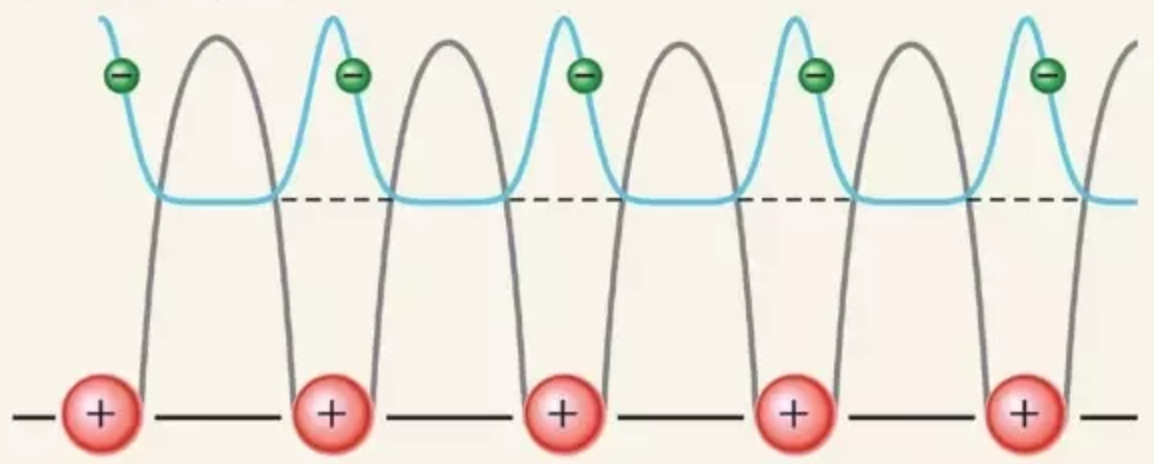
\includegraphics[scale=0.5]{figures/TightBoundModel1.png}
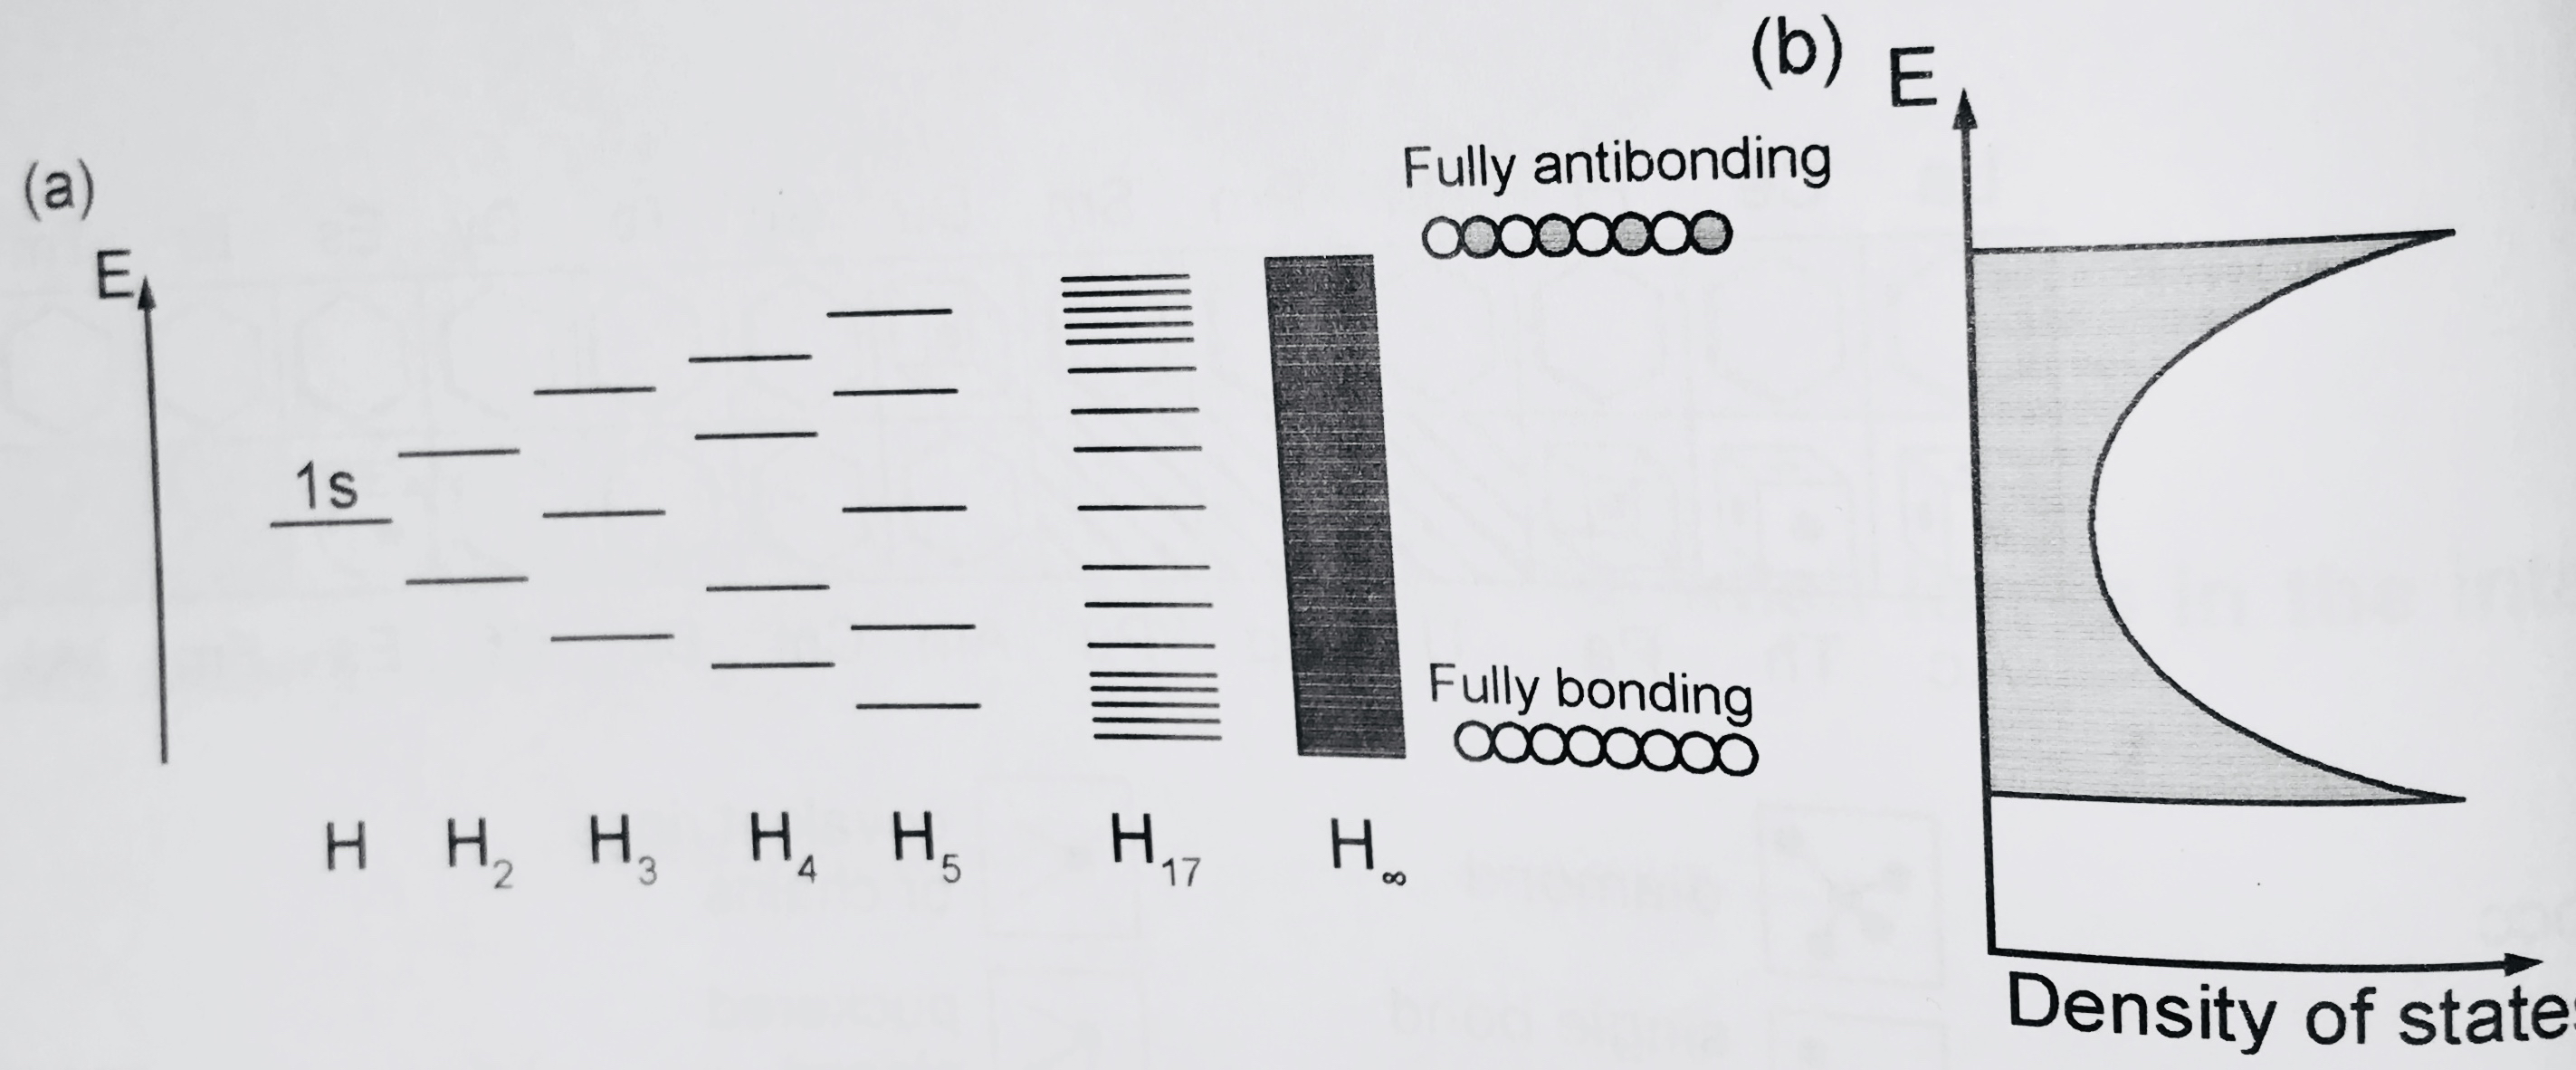
\includegraphics[scale=0.13]{figures/TightBoundModel2.png}
\caption[Tight Bound Model]{Tight Bound Model aplicat a l'estructura electrònica d'un metall. A dalt: podem considerar que cada electró està fortament lligat al seu nucli. A baix: estructura electrònica de considerar un conjunt molt gran d'àtoms d'hidrogen formant un hipotètic cristall metàl·lic; la suma dels orbitals electrònics forma un orbital molecular  amb un continu d'energies \cite{Yen2008}.}
\label{fig:TightBoundModel}
\end{figure}

Els electrons disposats d'aquesta manera ocupen orbitals atòmics que es combinen linealment seguint la teoria LCAO (la veurem més endavant) i generen el mateix nombre d'orbitals moleculars. En el cas d'un hipotètic cristall d'àtoms d'hidrogen obtindríem un diagrama energètic dels diferents orbitals fins a formar una banda com es mostra en la part inferior de la Figura \ref{fig:TightBoundModel}.

Un millor model és l'anomenat de l'electró lliure. 
En aquest model, es considera que els electrons es poden moure lliurement per l'estructura tridimensional del metall. 
Així, la quantitat d'electrons $N$ de massa $\mu$ que poden ser encabits en un nivell d'energia $E_{max}$ en un cub tridimensional de costat $a$ ve donat per:
\[
N=\frac{8 \pi a^3}{3} \left( \frac{2 \mu E_{max}}{h^2} \right)^{\frac{3}{2}}
\]
o, dit d'una altra manera, l'energia d'una determinada densitat d'electrons $\rho$ és:
\[E_{max} = \frac{h^2}{2 \mu} \left( \frac{3 \rho}{8 \pi} \right)^{\frac{2}{3}}\]

\begin{figure}[h]
\centering
\includegraphics[scale=0.08]{figures/FreeElectron.png}
\caption[Model de l'electró lliure]{En el model de l'electró lliure, la densitat d'estats d'un gas d'electrons és proporcional a l'arrel quadrada de l'energia cinètica de les partícules \cite{Yen2008}. }
\label{fig:FreeElectron}
\end{figure}

A 0K els electrons només ocupen els estats d'energia més baixos fins a l'anomenat nivell de Fermi (Figura \ref{fig:FreeElectron}). Els electrons addicionals que entrin al sistema a causa de la conducció elèctrica omplen els orbitals vacants.

Entre els orbitals ocupats i els orbitals vacants pot existir un gap que fa que a baixa temperatura aquests metalls no condueixin. Es necessita major temperatura per tal que tornin a ser conductors. 
És el que s'anomena un semiconductor. Veure Exercici \ref{Ex:Fermi}.

\begin{exr}
La funció de Fermi $f(E)$ dóna la probabilitat de que un determinat estat energètic sigui ocupat a una determinada temperatura superior a 0K:
\[f(E)=\left( 1 + \exp \left[ \frac{E-E_f}{k_B T} \right] \right)^{-1}\]
a) Dibuixa $f(E)$. b) Si el nivell de Fermi per al coure és de 7eV, raona com es distribuiran els seus electrons a 0K i a 1000K.
\label{Ex:Fermi}.
\end{exr}

\begin{figure}[h]
\centering
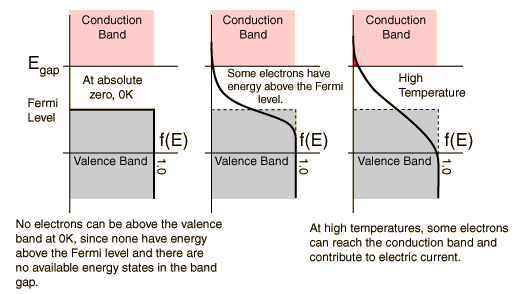
\includegraphics[scale=0.7]{figures/FermiBand.png}
\caption{Efecte de la temperatura en un semiconductor.}
\label{fig:FermiBand}
\end{figure}

\subsubsection{Cristalls iònics}
 Cada ió està lligat per una força Coulòmbica als altres i això fa que tinguin energies de dissociació (lattice energies) molt altes. 
\begin{equation}
U=-k\frac{Q_1 Q_2}{r_0} = \frac{NMz_+z_-e^2}{4\pi \varepsilon_0 r_0}
\label{Eq:Coulomb}
\end{equation}
Les energies depenen de la càrrega.
A l'Equació \ref{Eq:Coulomb}, M és l'anmenada constant de Madelung, que és fruït de considerar la interacció amb tota la resta d'ions que ocupen determinades posicions en la retícula.
\begin{figure}[h]
\centering
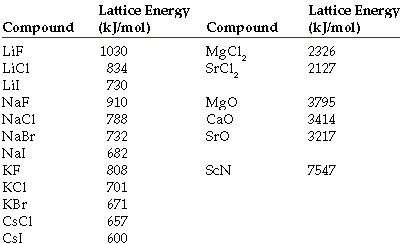
\includegraphics[scale=0.8]{figures/latticeEnergy.png}
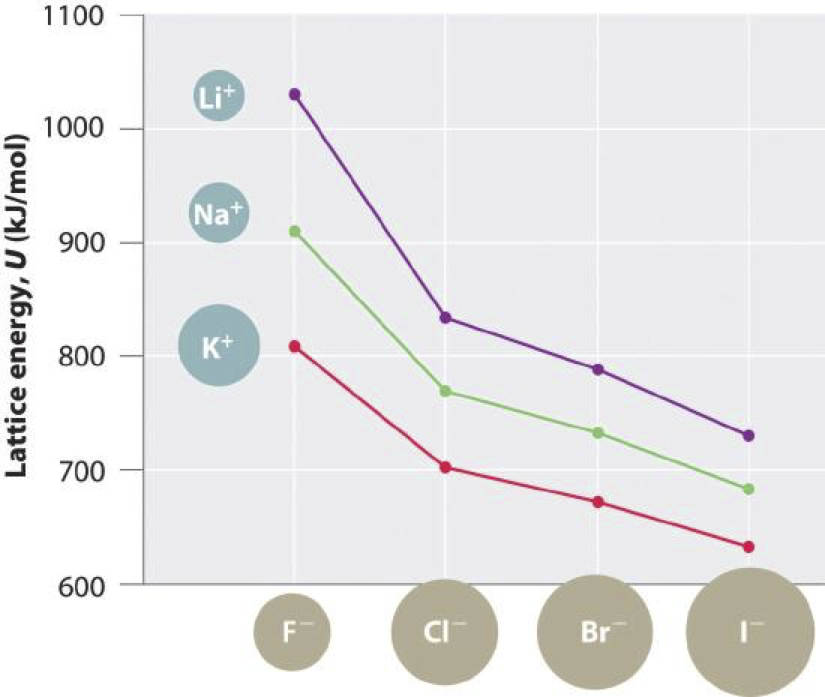
\includegraphics[scale=0.6]{figures/latticeEnergySize.png}
\caption{Energies reticulars (lattice energies) de diversos sòlids iònics.}
\label{fig:latticeEnergy}
\end{figure}
\begin{exr}
Ordena GaP, BaS, CaO, and RbCl per ordre de les seves energies de dissociació.
\end{exr}

\begin{exr}
Usant la descripció del Cicle de Born-Haber que trobaràs a la Wikipedia (\linkurl{https://ca.wikipedia.org/wiki/Cicle_de_Born-Haber}) calcula l'energia reticular del Fluorur de Liti.
\end{exr}

\subsubsection{Cristalls moleculars}

Formats per molècules covalents. 
\begin{itemize}
\item[no polars] Es mantenen units per forces de van der Waals de tipus dispersius.
\item[polars] Es mantenen units per unions de vdW dipol-dipol.
\item[ponts d'hidrogen] 
\end{itemize}  

\subsubsection{Sòlids covalents}

Tots els àtoms estan units per enllaços covalents (diamant, grafit). Veurem en seccions properes com es formen aquests enllaços.


\begin{exr}
Compara, per als diferents tipus de sòlids descrits, les següents característiques:
\begin{enumerate}
\item pressió de vapor
\item punt de fusió
\item punt d'ebullició
\item duresa
\item fragilitat
\item conducció elèctrica en estat sòlid
\item conducció elèctrica en estat líquid
\end{enumerate}
\end{exr}

\subsection{Defectes}

Les xarxes cristal·lines  incorporen gran nombre de defectes que, sovint, els donen les seves propietats més interessants. Hi ha diversos tipus de defectes en els cristalls:
\begin{description}
\item[Defectes de punt] Impliquen una sola posició (veure Figura \ref{fig:DefectesPunt}). Identifiquem els defectes de Schottky com aquells on apareixen vacants catió-anió en parelles. En un defecte de Frenkel, en canvi, hi ha un desplaçament d'un catiuó cap a una posició intersticial. En els dos casos es manté la neutralitat de l'estructura (a la fluorita, per exemple, els intersticis són grans, i per tant és fpacil trobar defectes de Frenkel). Si el defecte és l'absència d'un anió podem tenir un defecte de tipus centre F.
\item[Defectes de línea] Tenen a veure amb desplaçaments o alteracions d'una fila de posicions a la xarxa. Es poden provocar dislocacions d'aresta (de l'ordre de 10$^6$ per cm$^2$ en un metall templat o 10$^{12}$ per cm$^2$ en un metall treballat en fred.
\item[Defectes de pla] Bidimensionals. Els àtoms en l'extrem dels microcristalls poden ser més reactius per estar exposats amb més facilitat.
\end{description}

\begin{figure}[h]
\centering
\includegraphics[scale=0.1]{figures/DefectesPunt.png}
\caption{Diversos tipus de defecte de punt en un cristall.}
\label{fig:DefectesPunt}
\end{figure}

\begin{exr}
El coure té una estructura cúbica de cara centrada, i l'aresta de la cel·la unitària és de 3.61${\AA}$. Pots suggerir algun tipus d'àtom que es pugui col·locar en els  intersticis de la seva xarxa sense distorsionar-la?
\end{exr}

\begin{exr}
Si la densitat del clorur sòdic sense defectes és de 2.165 g cm$^{-3}$, quina seria la densitat si tingués un ratio de 10$^{-3}$ defectes de a) Frenkel; b) Schottky. (el volum no varia amb els defectes)
\end{exr}

%\subsection{Propietats tèrmiques (M)}

\section{Líquids i dissolucions}

\subsection{Teoria cinètica (M)}

Les partícules que conformen un líquid es poden moure en el seu sí, i Robert Brown (1827) va suggerir que feien de forma aleatòria. Això era degut a la petita mida de les partícules (de l'ordre de 10${-6}$m) i el constant xoc de les partícules que el formen.

\begin{figure}[h]
\centering
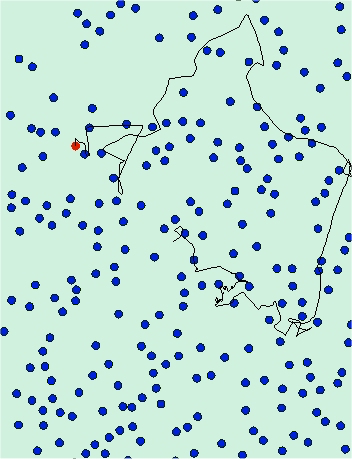
\includegraphics[scale=0.5]{figures/Brownian_motion.png}
\caption[Moviment Brownià]{Representació del moviment Brownià d'una partícula petita en un fluïd. La seva mida fa que els xocs amb les molècules del fluïd faci variar la seva trajectòria de forma globalment aleatòria.}
\label{fig:Brownian_motion}
\end{figure}

El moviment Brownià es pot representar per un model estocàstic en el qual els canvis de posició des d'un instant a l'altre estan produïts per moviments aleatoris extrets d'una distribució normal amb mitjana $\mu=0.0$ i variança $\sigma^2 \times \Delta t$, o $N(0,\sigma^2 \times \Delta t)$. En altres paraules, la variança augmenta amb el temps de forma lineal amb pendent $\sigma^2$. 

\begin{exr}
Usant R, prova d'executar aquest script que mostra com simular el moviment Brownià d'una partícula en un líquid (extret de \linkurl{http://www.phytools.org/eqg/phytools/}):
\begin{lstlisting}[language=R]
t <- 0:100  # temps de simulació
sig2 <- 0.01
## primer, calcula un conjunt de desviacions aleatòries puntuals
x <- rnorm(n = length(t) - 1, sd = sqrt(sig2))
## després, acumula'n els resultats
x <- c(0, cumsum(x))
plot(t, x, type = "l", ylim = c(-2, 2))
\end{lstlisting}

Després, executa el següent script, que produeix 10000 simulacions diferents:

\begin{lstlisting}[language=R]
nsim <- 1000
## creo una matriu que hostatgi totes les simulacions
X <- matrix(0, nsim, length(t))
for (i in 1:nsim) X[i, ] <- c(0, cumsum(rnorm(n = length(t) - 1, sd = sqrt(sig2))))
plot(t, X[1, ], xlab = "temps", ylab = "desviacions", ylim = c(-2, 2), type = "l")
for (i in 1:nsim) lines(t, X[i, ])
\end{lstlisting}
\end{exr}
\begin{exr}
Per saber la variança que s'obté de la simulació podem fer
\begin{lstlisting}[language=R]
var(X[, length(t)])
\end{lstlisting}
i per mostrar l'histograma de posicions finals:
\begin{lstlisting}[language=R]
hist(X[, length(t)])
\end{lstlisting}
o bé:
\begin{lstlisting}[language=R]
plot(density(X[, length(t)]))
\end{lstlisting}
Calcula la variança de la distribució per a diferents valors del nombre de simulacions o el temps simulat.
\end{exr}

A partir de la teoria cinètico-molecular es pot veure que l'energia mitjana de les partícules en un moviment Brownià és $3/2 RT$, la mateixa que la de les molècules d'un gas a la mateixa temperatura. Només cal pensar en què passa en la interfície d'un líquid i un gas a la mateixa temperatura.


\subsection{Equilibris de fase (M)}

El pas de líquid a vapor s'anomena \emph{vaporització}, i es pot donar a la superfície del líquid (\emph{evaporització}) o en tot el seu volum (\emph{ebullició}).
Es tracta d'un procés endotèrmic. El seu procés contrari és la \emph{condensació}.

\begin{exr}
Explica, segons la teoria cinètico-molecular, la Figura \ref{fig:evap_vs_condens}. Com interpretes els termes \emph{equilibri dinàmic} i \emph{saturació}?
\end{exr}
\begin{figure}[h]
\centering
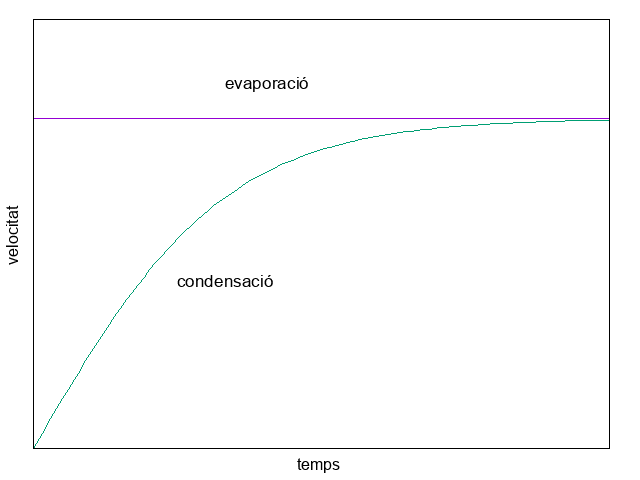
\includegraphics[scale=0.6]{figures/evap_vs_condens.png}
\caption{Esquema de la dependència de les velocitats d'evaporació i condensació respecte el temps en un líquid que s'evapora dins d'un recipient tancat.}
\label{fig:evap_vs_condens}
\end{figure}

La pressió que exerceix el vapor d'una substància a una temperatura determinada un cop és en equilibri amb la mateixa substància líquida és el que anomenem \emph{pressio de vapor} d'aquesta substància, $p_v$. La pressió de vapor augmenta en augmentar $T$, com es veu a la Figura \ref{fig:Water_vapor_pressure_graph}. Tots els líquids presenten corbes similars, amb pendent positiva.

\begin{figure}[h]
\centering
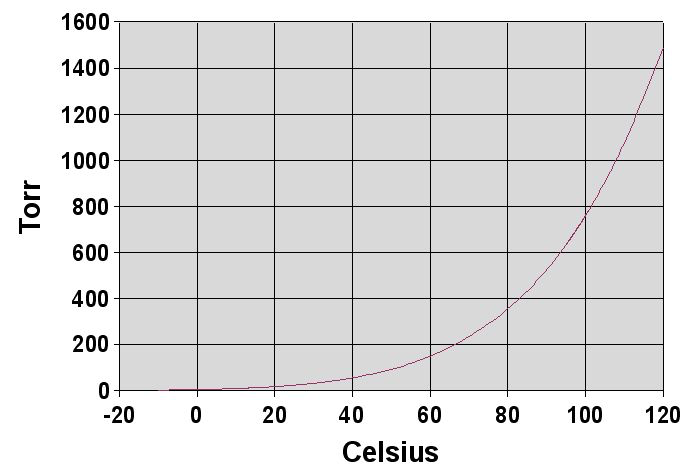
\includegraphics[scale=0.4]{figures/Water_vapor_pressure_graph.png}
\caption{Pressió de vapor de l'aigua en funció de la temperatura.}
\label{fig:Water_vapor_pressure_graph}
\end{figure}

La \emph{temperatura d'ebullició normal} és la que presenta un líquid a pressió 1 atm. La temperatura d'ebullició d'un líquid dependrà de la pressió exterior i de la natura del líquid.

\begin{exr}
És possible que un líquid arribi a estar sobreescalfat: temperatura superior a la d'ecullició per a aquella pressió però encara estat líquid, la qual cosa succeeix quan és molt pur i no hi ha partícules de pols.
Com aconseguiries que no es produeixi aquest sobreecalfament?
\end{exr} 

Hi ha una relació força directa entre la  pressió de vapor, la temperatura d'ebullició i la calor de vaporització (veure Taula \ref{tab:pv}). En general, com més intenses són les force sintermoleculars més alta és $\Delta H_v$ i $T_e$.
\begin{table}[h!]
  \begin{center}
    \caption{Pressió de vapor a 20$\degree$C, temperatura d'ebullició i calor de vaporització d'alguns líquids  (adaptat de \cite{Caamano1984}).}
    \label{tab:pv}
    \begin{tabular}{ccccc}
%    \begin{tabular}{ccS[table-format=2.4]S[table-format=4.1S[table-format=2.4]}
      \hline
      Líquid & naturalesa & $p_v$/10$^5$Pa & $T_e$/$\degree$C & $\Delta H_v$/kJ mol$^{-1}$\\
      \hline
      \ch{He} & no polar & $-$ & -268.9 & 0.1003 \\
      \ch{H2} & no polar & $-$ & -252.7 & 0.9028 \\
      \ch{CH4} & no polar & $-$ & -161.4 & 9.263 \\
      \ch{n-C4H10} & no polar & 2.03 & -1.5 & 24.24 \\
      \ch{CCl4} & no polar & 0.121 & 76.7 & 34.57 \\
      \ch{NH3} & polar & 10.1 & -33-6 & 20.15 \\
      \ch{H2O} & polar & 0.0233 & 100.0 & 40.62 \\
      \ch{CH3CH2OH} & polar & 0.0586 & 78.5 & 40.44 \\
      \ch{CH3OCH3} & polar & 5.06 & -23.7 & 22.61 \\
      \ch{CH3COCH3} & polar & 0.247 & 56.5 & 31.94 \\
      \hline
    \end{tabular}
  \end{center}
\end{table}

La Figura \ref{fig:hidrurs_boiling_point} mostra com la $T_e$ evoluciona en paral·lel a la taula periodica, i també com algunes substàncies són significativament excepcions d'aquesta norma degut a la seva capacitat d'establir ponts d'hidrogen.
\begin{figure}[h]
\centering
\includegraphics[scale=0.4]{figures/hidrurs_boiling_point.png}
\caption{Punts d'ebullició de diversos hidrurs relacionats amb la posició dels seus elements no metàl·lics a la taula periòdica.}
\label{fig:hidrurs_boiling_point}
\end{figure}

\subsection{Propietats crítiques}
\label{sec:PropietatsCritiques}

Michael Faraday va licuar gas clor el 1823, però per a altres gasos (\ch{H2}, \ch{N2} o \ch{O2}) no es va aconseguir i no va ser fins que Thomas Andrews va aconseguir liquar \ch{CO2} només si treballava a temperatures inferiors a 31$\degree$C. Així va sorgir el concepte de \emph{temperatura crítica}, $T_c$, com a propietat característica dels gasos, i que es defineix com aquella a partir de la qual no és possible liquar-los (veure Figura \ref{fig:punt_critic}).
En el punt crític, la $P_c$ és la pressió de vapor del líquid a $T_c$. És la màxima pressió de vapor del líquid, ja que a més $T$ no té sentit parlar-ne, ja que no existeix l'estat líquid. La corba de pressió front a la temperatura finalitza, doncs, en aquest punt.

\begin{figure}[h]
\centering
\includegraphics[scale=0.6]{figures/punt_critic.png}
\caption[Punt crític]{a) Cada corba isoterma representa la relació entre $P$ i $V$ a una temperatura donada. Les corbes inferiors deixen de sser hipèrboles perquè el gas es torna no ideal; b) el terme ``vapor'' es refereix a gas a una temperatura inferior al punt d'ebullició. Veure valors de punts crítics de substpancies comunes a \linkurl{http://philschatz.com/physics-book/contents/m42218.html}.\cite{Phase2018}}
\label{fig:punt_critic}
\end{figure}


\begin{figure}[h]
\centering
\includegraphics[scale=0.8]{figures/WaterPD.png}
\caption[Diagrama de fases simplificat de l'aigua]{Diagrama de fases simplificat de l'aigua. El gràfic no és a escala i tampoc conté diverses variants específiques que el farien molt complex.\cite{Phase2018}}
\label{fig:WaterPD}
\end{figure}
Al PC, la concentració molecular i tota la resta de propietats es fan iguals per al líquid i el gas.

\begin{exr}
Què ens produirà una cremada més gran: una massa $m$ d'\ch{H2O}(g) a 100 graus o la mateixa quantitat d'aigua líquida a la mateixa temperatura?
\end{exr}

\begin{exr}
En un recipient hi ha aigua líquida. Es conecta el frecipient a una bomba de buit i es va abaixant la pressió sobre el líquid. Si la temperatura és de 60 graus, a quina pressió bullirà l'aigua?
\end{exr}

\begin{exr}
Perquè a la Taula \ref{tab:pv} no apareix la $p_v$ de l'\ch{He}, \ch{H_2} i \ch{CH4}?
\end{exr}

A partir de tot el què hem treballat fins a aquest punt, queda clar que hi ha dues forces motores dels processos moleculars. D'una banda tots tendeixen a la mínima energia, però això no explicaria perquè els gasos existeixen com a tals. És necessari considerar la necessitat de tendir a un màxim desordre. El primer efecte ve determinat per l'entalpia del sistema i el segon per l'entropia. Ho treballarem més endavant amb major detall.

Ara com ara sí que podem, però determinar quatre característiques importants que tornarem a retrobar i formular:
\begin{enumerate}
\item L'equilibri en els sistemes moleculars és dinàmic, conseqüència de velocitats de reacció oposades.
\item El sistema passa espontàniament a l'estat d'equilibri.
\item Un cop assolit l'equilibri, les seves propietats són sempre les mateixes.
\item L'equilibri és fruit de dues tendències oposades: la necessitat d'assolir el mínim d'energia i la tendència al màxim caos.
\end{enumerate}

Això es pot escriure en base a l'energia lliure del procés d'equilibri. En equilibri, $\Delta G=\Delta H - T\Delta S0$, i per a tot procés espontani, $\Delta G <0$.
Més endavant anirem ampliant aquests conceptes termodinàmics, però ara com ara ens serveixen per entendre els fenòmens que hem anat explornat i que veure a continuació.

\subsection{Dissolucions}

Una dissolució és una substància complexa homogènia que, dins d'uns límits raonables, té una composició que pot variar contínuament.
Veurem més endavant que aquesta definició no és massa clara (pensem en el sabó en l'aigua).

La mesura de la concentració d'una dissolució pot donar-se en:
\begin{itemize}
\item \emph{Unitats de fracció molar.} $x_1=\frac{n_1}{n_1+n_2}$ i $x_2=\frac{n_2}{n_1+n_2}$
\item \emph{Molalitat} Número de mols de solut que hi ha en 1000g de solvent.
\item \emph{Molaritat} Número de mols per 1 litre de dissolució.
\item \emph{Normalitat} Número de pesos equivalents-gram del solut en un litre de dissolució.
\end{itemize}
\subsection{Solucions ideals i no ideals}

\begin{exr}
Raona com canvia la $p_v$ d´'una dissolució en funció de la seva concentració.
\end{exr}
Una dissolució ideal es forma sense despreniments de calor i amb una pressio de vapor que evoluciona segons la llei de Raoult:
\[
P_{dissolució}=P_{dissolvent}=P_1=P_1^0x_1 = P_1^0 \left(\frac{n_1}{n_1+n_2}\right)
\]
\begin{exr}
Determina la relació entre l'increment de pressió de vapor d'una dissolució i la fracció molar del solut.
\end{exr}
\begin{exr}
La pressió de vapor de l'aigua a 20$\degree$C és 17.54 mmHg. Quan dissolem 114g de sucrosa en 1000g d'aigua, la pressió de vapor es redueix en 0.11 mmHg. Quin és el pes molecular de la sucrosa?
\end{exr}

A partir de la llei de Raoult es pot arribar amb relativa facilitat a una expressió que relaciona la molalitat amb l'increment del punt d'ebullició:
\[
\Delta T=K_b m
\]
on $K_b$ és la constant d'elevació molal del punt d'ebullició respecte la concentració.
\begin{exr}
a) Exactament 1.00g d'urea dissolts en 75.00g d'aigua donen una dissolució que bull a 100.114$\degree$C. El pes molecular de la urea és 60.1. Quina és la $K_b$ de l'aigua?
b) Una dissolució preparada dissolent 12,00g de glucosa en 100g d'aigua bull a 100.34$\degree$C. Quin és el pes molecular de la glucosa?
\end{exr}
Quelcom similar es pot deduir per al punt de fusió: \[\Delta T = K_f m\]. Cal notar que, si en lloc de només un solut n'hi ha més d'un, hem de tenir en compte la molalitat total de la dissolució.

En el cas de tenir més d'un component volàtil a la dissolució, només hem de tenir present que la llei de Raoult s'acomplirà per a totes dues, i per tant la pressió parcial de cadascuna de les dues substàncies volàtils s'haurà de sumar:
\[
P_T=P_1+P_2=x_1P_1^0+x_2P_2^0
\]

En una dissolució ideal de dues components, el vapor sempre es troba enriquit amb aquella de les dues substàncies que sigui més volàtil.
A partir de la diferència de volatilitat de dos components en una dissolució podem analitzar la composició del vapor fent servir diagrames com el de la Figura \ref{fig:PhaseDiagram}a.
Usant aquesta mena de diagrames podem estudiar la destil·lació fraccionada d'una dissolució líquida de dues substàncies volàtils (Figura \ref{fig:PhaseDiagram}b).

\begin{figure}[h]
\centering
\includegraphics[scale=0.5]{figures/PhaseDiagram.png}
\includegraphics[scale=0.5]{figures/FractionalDistillation.png}
\caption[Diagrama de fases i destil·lació fraccionada d'una dissolució ideal]{a) La corba inferior mostra el punt d'ebullició d'una dissolució ideal per a diferents composicions. La corba superior mostra la composició del vapor, si connectem, per a una $T_{ebullició}$ d'ebullició donada, els punts de tall de les dues corbes a aquesta $T$. b) Destil·lació fraccionada d'una disslució ideal.}
\label{fig:PhaseDiagram}
\end{figure}

En una dissolució ideal no es desprèn ni absorbeix calor ($\Delta H=0$) i per tant, el procés és purament entròpic, cosa que el fa espontani (si $\Delta H=0$, $\Delta G= -T \Delta S<0$).

En dissolucions no ideals, observem una desviació respecte la llei de Raoult que pot ser positiva o negativa (veure, per exemple, \linkurl{https://www.youtube.com/watch?v=4hmrDSxEN-Q} o la Figura \ref{fig:desv_raoult}).
\begin{figure}[h]
\centering
\includegraphics[scale=1.0]{figures/desv_raoult.png}
\caption[Llei de Raoult per dissolucions ideals i no ideals]{a) en una desviació positiva respecte la llei de Raoult, els dos líquids que formen la barreja les forces d'atracció entre les dues substàncies són menors que les que es produeixin dins d'una d'elles: A i B escapen fàcilment i mostren, per tant, major pressió de vapor que l'esperada; b) en una desviació negativa, els dos líquids mostren una atracció mútua més gran que en cadascun per separat: les substàncies A i B tendeixen a marxar de la dissolució menys que en la situació ideal.}
\label{fig:desv_raoult}
\end{figure}

És interessant separar les dissolucions entre aquelles que:
\begin{itemize}
\item Desprenen calor en formar-se ($\Delta H <0$). Per exemple, si dissolem cloroform (\ch{CHCl3}) en acetona (\ch{(CH3)2CO}), es desprèn calor, en tant que es formen ponts d'hidrogen entre les molècules dels dos tipus de substància, però no dins de cadascuna d'elles (veure Figura \ref{fig:CloroformAcetona}).
\begin{figure}
  \centering
\chemfig{Cl>:[,1.2]C(<[3,1.2]Cl)(<[5,1.2]Cl)(-[0]H-[,,,,dash pattern=on 2pt off 2pt]O=C(-[1]CH_3)(-[7]CH_3))}
(\cmpd{cpmd:CloroformAcetona})\par
  \caption{La interacció de pont d'hidrogen entre el cloroform i l'acetona provoca un comportament no ideal de la llei de Raoult.}
  \label{fig:CloroformAcetona}
\end{figure}
En aquest cas, la pressió de vapor serà menor a l'esperada a partir de la llei de Raoult (Figura \ref{fig:desv_raoult}b). 
\item Absorbeixen calor en formar-se ($\Delta H > 0$). Això succeeix en els casos en els què barregem sbstàncies polars amb no polars i, per tant, eliminem moltes interaccions que altrament ja serien prou favorables. Per exemple, si barregem acetona (veure estructura a \ref{cpmd:ClorofomAcetona}) amb bisulfur de carboni (\chemfig{S=C=S}). Veure Figura \ref{fig:desv_raoult}a)
\end{itemize} 
Per tant, si la $T$ canvia en fer una dissolució de dues substàncies, la dissolució és no ideal.
Si observem amb atenció la Figura \ref{fig:desv_raoult} veiem que en el límit de dilució (dilució infinita) el corresponent dissolvent es comporta de forma propera a la ideal.

En una dissolució no ideal de dos components, a diferència del què passava amb les dissolucions idelas, no sempre el vapor es troba enriquit amb la substància més volàtil. 

\begin{exr}
Raona l'efecte que té la no idealitat de les dissolucions segons la Figura \ref{fig:desv_raoult}a a) en el seu punt d'ebullició, i b) en un procés de destil·lació fraccionada.
\end{exr}

Les dissolucions que destil·len sense canvi en la composició s'anomenen azeòtropes. Per exemple, si fem una barreja d'agua i àcid clorhídric i la fem bullir un temps suficient, la seva composició arribarà a un pes d'\ch{HCl} del 20.22\% respecte el pes total.

\begin{exr}
Un azeòtrop positiu prové d'una desviació també positiva de la llei de Raoult. a) Dibuixa la corba de Temperatura d'ebullició vs composició per a un azeòtrop positiu basant-te en les Figures \ref{fig:PhaseDiagram}a i \ref{fig:desv_raoult}a. b) Raona el resultat de fer una destil·lació a partir de diverses composicions d'aquesta mescla. c) què succeiria en un azeòtrop negatiu?
\end{exr}
\begin{figure}[h]
\centering
\includegraphics[scale=1.0]{figures/AzeotropEX.png}
\caption{Dades per al sistema etanol - acetat etílic (extret de \cite{Robin2016}).}
\label{fig:AzeotropEX}
\end{figure}
\begin{exr}
Volem separar una barreja equimolar d'etanol i acetat etílic per destil·lació en productes relativament purs. La barreja forma un azeòtrop de mínim punt d'ebullició segons la Figura \ref{fig:AzeotropEX}. No obstant, la composició de l'azeòtrop és sensible a la pressió, mostrant un increment significatiu de la fracció molar de l'etanol quan incrementa la pressió, com es mostra a la Figura. Dibuixa un esquema aproximat per a la separació de les dues components de la barreja que tregui profit d'aquest fet.
\end{exr}

\subsection{Solubilitat}

En la majoria dels casos, dues substàncies no es poden dissoldre l'una en l'altra en qualsevol proporció.
La solubilitat d'una substància en un determinat dissolvent, a una temperatura donada, és la concentració del solut en la dissolució saturada.
És una propietat fonamental per separar components d'una dissolució.
La solubilitat depèn de la natura de dissolvent i solut, així com de la $T$ i la $P$.

Per entendre l'efecte de la $T$ en la solubilitat usarem l'anomenat principi de LeChatelier, segons el qual "si s'exerceix alguna acció sobre un sistema que inicialment està en equilibri que afecti algun dels factors que l'identifiquen com a tal, el sistema es regularà ell mateix de manera que tendeixi a reduir l'efecte d'aquell canvi".
\begin{exr}
Raona perquè per a una dissolució en la qual $\Delta H_{sol} <0$, un augment de la temperatura fa que la solubilitat disminueixi, i a l'inrevés.
\end{exr}

Es pot relacionar les pressió d'un gas i la seva solubilitat a una $T$ donada en un líquid segons la llei de Henry\footnote{William Henry, 1775-1836}:
\[
C=kP
\]
on $C$ és la concentració (M) del gas en el líquid, $P$ la pressió parcial del gas i $k$ la constant de Henry, que depèn de la $T$ i la natura de gas i dissolvent (veure Taula \ref{tab:Henry}).

\begin{table}[h!]
  \begin{center}
    \caption{Constants de la llei de Henry per a diferents gasos en aigua a 20$\degree$C.}
    \label{tab:Henry}
    \begin{tabular}{cc}
      \hline
      Gas & constant de Henry / mol l$^{-1}$ atm$^{-1}$ \\
      \hline
He &	3.9\\
Ne &	4.7\\
Ar &	15\\
H2 &	8.1\\
N2 &	7.1\\
O2 &	14\\
CO2& 	392\\      
      \hline
    \end{tabular}
  \end{center}
\end{table}
% \chapter{Estructura electrònica dels àtoms i propietats periòdiques}

\section{L'estructura electrònica dels àtoms}
\subsection{Radiació d'un cos negre}
\begin{figure}[h]
\centering
\includegraphics[scale=0.5]{figures/blackbody.png}
\caption{Distribució de freqüències de radiació emeses per un cos negre}
\label{fig:blackbody}
\end{figure}
Rayleigh (Juny 1900). Radiació contínua $\lambda \nu = c$:
\[
R(\nu)=\frac{2 \pi k T}{c^2} \nu^2
\]
Planck (Octubre-Desembre 1900). Radiació en paquets $h\nu$ (\textit{quantum}):
\[
R(\nu)=\frac{c_1 \nu^3}{e^{c_2 \nu T} -1}=\frac{2\pi h \nu^3}{c^2} \frac{1}{e^{h\nu/kT}-1}
\]
\subsection{Efecte fotoelèctric i experiment de Rutherford}
\begin{figure}[h]
\centering
\includegraphics[scale=1.5]{figures/photoelect.png}
\caption{Efecte fotoelèctric}
\label{fig:photoelect}
\end{figure}
Lenard (Nobel 1905, raigs catòdics):
\begin{enumerate}
\item La freqüència llindar $\nu_0$ d'emissió depèn de cada metall
\item més llum, més electrons, però amb la mateixa energia cinètica
\item Més freqüència de radiació més energia cinètica electrons
\end{enumerate}
Einstein (1905):
\[
E_{fotó}=h \nu
\]
\[
h\nu = W + 1/2 m v^2
\]
Però per explicar-ho implicava introduir el concepte de dualitat ona-corpuscle.

Des dels experiments de Thomson amb raigs catòdics (1897) i Milikan (1909) es sabia que els àtoms estaven formats per càrregues positives i negatives, però es pensava que tenien forma esfèrica amb els electrons al seu interior.
\begin{figure}[h]
\centering
\includegraphics[scale=0.5]{figures/Rutherford.png}
\caption[Model de Rutherford]{La figura de l'esquerra mostra com haurien de travessar una placa metàl·lica partícules $\alpha$ segons el model de Thomson, A la dreta de la figura apareix l'explicació del comportament experimental real segons el model de Rutherford.}
\label{fig:Rutherford}
\end{figure}
Rutherford (1911) va mostrar que l'àtom no podia ser una esfera uniforme com la predita. Va mostrar que fent impactar partícules $\alpha$ (nuclis d'àtoms d'heli; per tant, amb càrrega +2 i massa 4) sobre una placa fina de metall es produïa ampla difracció d'un nombre petit de partícules i n'hi havia moltíssimes que travessaven la placa sense cap desviació o ben poca. Això implicava que els àtoms havien d'estar formats per una massa central altament carregada positivament i havien de tenir un volum molt més gran per tal que les partícules majoritàriament travessessin la placa (Figura \ref{fig:Rutherford})\footnote{\linkurl{https://commons.wikimedia.org/wiki/File:Geiger-Marsden_experiment_expectation_and_result.svg}}.

\subsection{Àtom de Bohr}
\begin{figure}[h]
\centering
\includegraphics[scale=0.7]{figures/Bohr.png}
\caption{Model de l'àtom de Bohr}
\label{fig:Bohr}
\end{figure}
Balmer, Rydberg (1885-1910); freqüències espectrals per a l'àtom d'hidrogen:
\begin{equation}
\frac{\nu}{c}=\frac{1}{\lambda}=R\left( \frac{1}{n_b^2}-\frac{1}{n_a^2}\right)
\label{eq:rydberg}
\end{equation}
\[
n_b=1,2,3,\dots; \; n_a=2,3,4,\dots; n_a>n_b
\]
on R=109677.6 cm$^{-1}$.

Bohr (1913):
\begin{enumerate}
\item estats estacionaris de l'àtom d'H
\item un estat estacionari no emet energia electromagnètica
\item l'emissió entre estats és igual a un fotó: $E_a-E_b=h\nu$.
\end{enumerate}
A partir de l'Eq. \ref{eq:rydberg} i aquest resultat, es pot veure que l'energia dels estats estacionaris del H ve donada per $E=-Rhc/n^2$ amb $n=1,2,3,\dots$. I va afegir dos postulats més al seu model:
\begin{enumerate}
\item l'electró de l'estat estacionari es mou en un cercle de radi determinat
\item hi ha una relació entre el radi d'aquestes òrbites i la seva energia $mvr=\frac{nh}{2\pi}$
\end{enumerate}
A partir d'aquí, va deduir una energia per a cada nivell d'energia:
\[
E=\frac{-2\pi^2 m e'^4}{h^2n^2}
\]
i $R=\frac{-2\pi^2 m e'^4}{h^3c}$. El resultat concorda amb l¡experiment i dóna els nivells correctes de les energies de l'àtom de Bohr, però els dos darrers postulats són totalment falsos i va ser el 1926 quan Schrödinger va formular la seva equació de la mecànica quàntica que superava el model de Bohr.

\subsection{Hipòtesi de de Broglie i principi d'incertesa}
El 1923, de Broglie va formular la hipòtesi de que la matèria, com la llum, també tenia naturalesa dual ona-corpuscle. 
Això explicaria el rerafons del model de Bohr: els electrons mostraven nivells d'energia quantitzats.
En el cas de la llum, Einstein havia arribat a que la relació entre la longitud d'ona i la massa d'un fotó era $\lambda=h/mc$. De Broglie va aplicar el mateix raonament a una partícula de massa $m$ i velocitat $v$: $\lambda=h/mv$.

A partir de considerar aquesta hipòtesi i la natura dual de les partícules, es pot arribar a veure que el producte de les incerteses en el càlcul de la posició i el moment lineal estan relacionades per $\Delta x \Delta p_x \geq h$, o principi d'incertesa de Heisenberg (1927).

\subsection{Mecànica quàntica}

Descrita per Heisenberg, Born i Jordan (1925) i per Schrödinger (1926). 

La mecànica clàssica és determinista, mentre que la quàntica és probabilística (pel principi d'incertesa de Heisenberg). L'Estat d'un sistema es determina per la seva funció d'estat $\Psi$, que és una funció de les coordenades de les partícules i del temps:
\begin{eqnarray}
-\frac{\hbar}{i} \frac{\partial \Psi}{\partial t}&=&-\frac{\hbar^2}{2m_1}\left(\frac{\partial^2\Psi}{\partial x_1^2}+\frac{\partial^2\Psi}{\partial y_1^2}+\frac{\partial^2\Psi}{\partial z_1^2} \right)-\\
 & & \cdots -\frac{\hbar^2}{2m_n}\left(\frac{\partial^2\Psi}{\partial x_n^2}+\frac{\partial^2\Psi}{\partial y_n^2}+\frac{\partial^2\Psi}{\partial z_n^2} \right) + V \Psi
\end{eqnarray}
on $\hbar=h/2\pi$, $i=\sqrt{-1}$, $m_1,\dots , m_n$ són les masses de les $n$ partícules de coordenades $x_i,y_i,z_i$ i $V$ és l'energia potencial del sistema.

El que ens interessa ara mateix és saber que la funció d'estat ens informa sobre l'estat del sistema.
A partir d'ella ho podem saber tot del sistema. El problema és trobar-la...

Per fer un cas senzill pensem en un sistema en el què l'energia potencial sigui independent del temps, com succeeix en un pàtom o una molècula aïllats. En aquest cas, l'equació es redueix a (per a una sola partícula)
\[
-\frac{\hbar^2}{2m}\frac{d^2 \psi(x)}{dx^2}+V(x)\psi(x)=E\psi(x)
\label{Eq:Schr1x}
\]
on $\psi$ és la funció d'ona del sistema.
\begin{figure}[h]
\centering
\includegraphics[scale=0.6]{figures/ParticulaCaixa.png}
\caption{Partícula en una caixa unidimensional de potencial $V=0$ entre $x=0$ i $x=L$ i $V=\infty$ en qualsevol altre posició}
\label{fig:ParticulaCaixa}
\end{figure}
\begin{mdframed}[backgroundcolor=gray!30,frametitle=Partícula en una caixa]
Un dels sistemes més simples per als quals l'Eq. \ref{Eq:Schr1x} es pot solucionar és el cas d'una partícula en una caixa unidimensional de parets infranquejables i impenetrables.
Considerem una partícula de massa $m$ que es mou amb una energia $E$ positiva al llarg de l'eix $X$ entre $x=0$ i $x=L$ (Figura \ref{fig:ParticulaCaixa}).
A partir de l'Eq. \ref{Eq:Schr1x} obtenim, per a aquest sistema:
\[
-\frac{}{2m}\frac{d^2 \psi}{dx^2}+V\psi(x)=E\psi
\]
Ens adonem que per a la regió $0\leq x \leq L$, on $V=0$, podem escriure:
 \[
\frac{d^2 \psi}{dx^2}=-\frac{2mE}{\hbar^2}\psi
\label{Eq:PC1}
\]
Com sabem, la segona derivada d'una funció $\psi$ ens dona informació qualitativa sobre la seva corbatura. En aquest cas veiem que quan la $\psi$ sigui negativa la seva corbatura serà positiva, i a l'inrevés. La funció $\sin(x)$ és un exemple d'aquest tipus de funció. De fet, $\psi=A \sin(bx)$ és una solució de l'Eq. \ref{Eq:PC1}. Si la substituïm a l'equació:
\begin{eqnarray*}
\psi = A \sin{bx} \\
\frac{d \psi}{d x} = bA \cos{bx} \\
\frac{d^2 \psi}{dx^2}=-b^2A \sin{bx}=-b^2 \psi
\label{Eq:PC2}
\end{eqnarray*}
Per tant, $\psi=A \sin{\left( \frac{2mE}{\hbar^2}\right)^{1/2} x}$. Fixem-nos que l'energia fins ara no està quantitzada, ja que no hem "tancat" la partícula restringint-la, encara, a cap valor, sinó que és un valor qualsevol positiu. Si ara tenim en compte que aquesta partícula no és lliure de moure's sinó que està tancada entre les parets $x=0$ i $x=L$ la situació canvia. Així, en tant que el quadrat de la funció d'ona es fa zero quan la probabilitat de trobar una partícula en un punt determinat és zero, i tenint en compte que la funció $\psi$ ha de ser contínua en tots els punts, és fàcil adonar-se que $\psi(x=0)=0$ i $\psi(x=L)=0$, que corresponen a les condicions límits del problema amb què ens enfrontem. La primera condició s'acompleix de forma automàtica si substituïm $x=0$ a l'Eq. \ref{Eq:PC2}. La segona condició, però, només s'acompleix si $\left( \frac{2mE}{\hbar^2}\right)^{1/2} L=n \pi$, amb $n=1,2,3,\ldots$. Els valors d'$E$ que compleixen aquesta condició són 
\[
E_n=\frac{n^2h^2}{8mL^2}, \; n=1,2,3,\ldots
\]
que representen els valors permesos (quantitzats) d'energia, corresponents a funcions d'ona del tipus:
\[
\psi_n=A \sin{\left( \frac{2mE_n}{\hbar^2}\right)^{1/2} x}=A \sin{\frac{n\pi x}{L}}
\]
Finalment, podem trobar $A$ tenint en compte que la probabilitat total de trobar la partícula en tot l'espai accessible $x\in [0,L]$ és igual a 1. Fent $\int_0^L \psi^2_n dx =1$ trobem que $A=\left( \frac{2}{L} \right)^{1/2}$. Per tant, finalment, els resultats de l'energia i la funció d'ona d'una partícula en una caixa són:
\begin{eqnarray}
E_n=\frac{n^2h^2}{8mL^2}\\
\psi_n= \left( \frac{2}{L} \right)^{1/2} \sin{\frac{n\pi x}{L}}
\end{eqnarray}
La Figura \ref{fig:ParticulaCaixa2} mostra la forma de la funció d'ona per als primers nivells de quantització de l'energia.\footnote{\linkurl{https://en.wikipedia.org/wiki/Particle_in_a_box}}
\end{mdframed}
\begin{figure}[h]
\centering
\includegraphics[scale=0.3]{figures/ParticulaCaixa2.png}
\caption{Funcions d'ona corresponents als primers nivells d'energia d'una partícula en una caixa unidimensional.}
\label{fig:ParticulaCaixa2}
\end{figure}
De l'exemple de la partícula en una caixa podem extreure'n conceptes generals que ens serviran més endavant:
\begin{itemize}
\item Els nivells d'energia quantitzats només apareixen si confinem la partícula entre dos extrems de potencial infinit. Sempre que tinguem moviments confinats o periòdics, apareixerà quantització, com en la rotació d'una molècula.
\item A mesura que augmenta la massa de la partícula o disminueix l'espai en el què aquesta està confinada, la distància entre les energies de quantització es fa menor.
\item El fet que la funció d'ona passi de valors positius a negatius implica que hi ha punts en els quals el seu valor és zero (i que anomenem \textit{nodes}). En aquests punts, el seu quadrat també serà zero, i per tant la probabilitat de trobar-hi la partícula serà nul·la.
\end{itemize}
\section{L'àtom d'hidrogen}

\subsection{Números quàntics}
Estudiar l'àtom d'hidrògen, l'exemple més simple possible, ens permetrà comprendre la base de l'enllaç químic entre àtoms.
L'aplicació de l'equació de Schrödinger 
\begin{equation}
H\Psi = E\Psi
\label{Eq:Schr}
\end{equation}a aquest àtom dóna resultats que estan d'acord amb les dades experimentals que se'n tenen.
L'equació de Schrödinger té la virtut de no necessitar postular els números que descriuen la quantització de l'energia, com succeïa en el model de Bohr. A partir d'aquesta equació, els números de la quantització de l'energia sorgeixen de forma natural en solucionar-la. En el cas de l'àtom d'hidroegn, els números quàntics que sorgeixen són:
\begin{description}
\item[Número quàntic principal, $n$]  Determina les energies accessibles per l'àtom d'hidrogen o per qualsevol altre àtom d'un sol electró i càrrega nuclear $Z$:
\[
E=-\frac{2\pi^2 me^4 Z^2}{n^2 h^2}
\]
$n=1,2,3\ldots$
Aquest resultat s'obté de la resolució de l'Eq. \ref{Eq:Schr} i és el mateix que va trobar Bohr en el seu model.
Cal fixar-se que l'energia en un àtom d'hidrogen o en qualsevol àtom en el qual només hi hagi un electró només depèn del número atòmic $n$.
\item[Número quàntic del moment angular, $l$] En estar relacionat amb el moment angular de l'electró, també ho està amb la seva energia cinètica i, per tant, és lògic que estigui limitat pel valor de $n$ (que expressa els nivells permesos d'energia total). $l=0, 1, \ldots, n-1$.
\item[Número quàntic magnètic, $m_l$] Pel fet que un electró amb un determinat moment angular pot ser considerat com un corrent elèctric que cirsula en un anell, pot generar un camp magnètic associat a aquest corrent. Aquest camp magnètic, pel fet d'estar associat al moment angular, estarà limitat al valor d'$l$: $m_l=-1, -l+1, \ldots, 0, 1, \ldots, l-1,l$.
\item[Número quàntic d'spin, $m_s$] Mostra la propietat magnètica intrínseca de l'electró i la possibilitat de girar sobre el seu eix en un sentit o un altre: $m_s=\{+\frac{1}{2},-\frac{1}{2}\}$.
\end{description}

\section{Orbitals moleculars}
El nivell d'energia $n$ determina les possibilitats dels altres números. Per exemple, en l'estat fonamental, l'àtom d'hidrogen pot tenir les combinacions de $\{n,l,m_l,m_s\}$ $\{1,0,0,+\frac{1}{2}\}$ i $\{1,0,0,-\frac{1}{2}\}$. De la mateixa manera, podem pensar en els estats excitats de l'àtom d'hidrogen considerant altres valors dels números quàntics, de manera que anem determinant els diversos orbitals :
\begin{table}[h!]
  \begin{center}
    \caption{Números quàntics i orbitals \cite{Mahan1977}}
    \label{tab:quant}
    \begin{tabular}{cccccc}
      \hline
      $n$ & $l$ & Orbital & $m_l$ & $m_s$ & combinacions\\
      \hline
      1 & 0 & 1s & 0 & $+\frac{1}{2},-\frac{1}{2}$ & 2 \\
      2 & 0 & 2s & 0 & $+\frac{1}{2},-\frac{1}{2}$ & 2 \\
      2 & 1 & 2p & $+1,0,-1$ & $+\frac{1}{2},-\frac{1}{2}$ & 6 \\
      3 & 0 & 3s & 0 & $+\frac{1}{2},-\frac{1}{2}$ & 2 \\
      3 & 1 & 3p & $+1,0,-1$ & $+\frac{1}{2},-\frac{1}{2}$ & 6 \\
      3 & 2 & 3d & $+2,+1,0,-1,-2$ & $+\frac{1}{2},-\frac{1}{2}$ & 10 \\
      4 & 0 & 4s & 0 & $+\frac{1}{2},-\frac{1}{2}$ & 2 \\
      4 & 1 & 4p & $+1,0,-1$ & $+\frac{1}{2},-\frac{1}{2}$ & 6 \\
      4 & 2 & 4d & $+2,+1,0,-1,-2$ & $+\frac{1}{2},-\frac{1}{2}$ & 10 \\
      4 & 3 & 4f & $+3,+2,+1,0,-1,-2,-3$ & $+\frac{1}{2},-\frac{1}{2}$ & 14 \\
      \hline
    \end{tabular}
  \end{center}
\end{table}

Per a un interessant i complet resum d'aquest capítol, ves a \linkurl{https://2012books.lardbucket.org/books/principles-of-general-chemistry-v1.0/s10-05-atomic-orbitals-and-their-ener.html}.
\begin{figure}[h]
\centering
\includegraphics[scale=0.4]{figures/SphericalCoords.png}
\caption{Coordenades esfèriques.}
\label{fig:SphericalCoords}
\end{figure}
A partir de la probabilitat de trobar un electró en un punt de l'espai, que ve donat per $\|\psi^2\|=1$ podem trobar la forma de les regions que ocuparà per a cada orbital (per analogia a les òrbites del model de Bohr). Si les expressem en coordenades esfèriques (Figura \ref{fig:SphericalCoords}) les funcions d'ona corresponents a cada orbital es poden expressar com a producte d'una part angular $\xi$ i una radial $R$ (veure Taula \ref{tab:AngRadOrb}).
\begin{equation}
\psi(r,\theta,\phi)=R_{n,l}(r)\chi_{l,m}(\theta,\phi)=R(r)\chi(\theta,\phi)
\label{Eq:psisplit}
\end{equation}
\begin{table}[h!]
  \begin{center}
    \caption{Part radial i part angular  de les funcions d'ona de l'àtom d'hidrogen \cite{Mahan1977}. $a=0$ és el radi de Bohr, $0.529 \times 10^{-10}$m.}
    \label{tab:AngRadOrb}
    \begin{tabular}{cc}
      \hline
      $\chi(\theta,\phi)$ & $R(r)$ \\
      \hline
      $\chi(s)=\left(\frac{1}{4\pi}\right)^{1/2}$ & $R(1s)=2 \left(\frac{Z}{a_0}\right)^{3/2} e^{-\sigma/2}$ \\
      \hline
$\begin{array}{rcl}
\chi (p_x)&=&\left(\frac{3}{4\pi}\right)^{1/2}\sin \theta \cos \phi \\
\chi (p_y)&=&\left(\frac{3}{4\pi}\right)^{1/2}\sin \theta \sin \phi \\
\chi (p_z)&=&\left(\frac{3}{4\pi}\right)^{1/2}\cos \theta 
\end{array}$
&
$\begin{array}{rcl}
R(2s) &=& \frac{1}{2\sqrt{2}}\left(\frac{Z}{a_0}\right)^{3/2} (2-\sigma) e^{-\sigma/2} \\
R(2p) &=& \frac{1}{2\sqrt{6}}\left(\frac{Z}{a_0}\right)^{3/2} \sigma e^{-\sigma/2} 
\end{array}$\\
      \hline
      $\begin{array}{rcl}
\chi (d_{z^2})&=&\left(\frac{5}{16\pi}\right)^{1/2} (3 cos^2 \theta -1) \\
\chi (d_{xz})&=&\left(\frac{15}{4\pi}\right)^{1/2}\sin \theta cos \theta \cos \phi \\
\chi (d_{yz})&=&\left(\frac{15}{4\pi}\right)^{1/2}\sin \theta cos \theta \sin \phi \\
\chi (d_{x^2-y^2})&=&\left(\frac{15}{4\pi}\right)^{1/2} \sin^2 \theta \cos 2\phi \\
\chi (d_{xy})&=&\left(\frac{15}{4\pi}\right)^{1/2} \sin^2 \theta \sin 2\phi \\
\end{array}$
&
$\begin{array}{rcl}
R(3s) &=& \frac{1}{9\sqrt{3}}\left(\frac{Z}{a_0}\right)^{3/2} (6-6\sigma +\sigma^2) e^{-\sigma/2} \\
R(3p) &=& \frac{1}{9\sqrt{6}}\left(\frac{Z}{a_0}\right)^{3/2} \sigma (4-\sigma) \sigma e^{-\sigma/2} \\
R(3d) &=& \frac{1}{9\sqrt{30}}\left(\frac{Z}{a_0}\right)^{3/2} \sigma^2 e^{-\sigma/2} 
\end{array}$\\
      \hline
      & $\sigma=\frac{2Zr}{na_0}; \; a_0=\frac{h^2}{4\pi^2 m e^2}$\\
      \hline
    \end{tabular}
  \end{center}
\end{table}

A partir de la Taula \ref{tab:AngRadOrb} es poden obtenir les funcions d'ona de tots els orbitals de l'àtom d'hidrogen. Per exemple, per a l'orbital 1s tenim:
\[
\psi(1s)= \frac{1}{\pi^{1/2}} \left( \frac{Z}{a_0} \right)^{3/2} e^{-Zr/a_0}
\]
i dóna una probabilitat de trobar l'electró a una distància $r$ de
\[
\psi^2(1s)= \frac{1}{\pi} \left( \frac{Z}{a_0} \right)^{3} e^{2Zr/a_0}
\]
que mostra com, en un orbital 1s, la màxima probabilitat de trobar l'electró es dóna a prop del nucli, i és independent de l'angle. 

\begin{exr}
Quants nodes té la funció $\psi(2s)$? i la $\psi(3s)$? i la $\psi(2p)$? 
\end{exr}
Com a norma, el número de nodes que podem trobar és $n-1-l$. 
En afegit, i per entendre millor la distribució electrònica, podem pensar en la densitat de probabilitat radial.
Aquesta es calcula trobant, a partir de la integració de l'expressió \ref{Eq:psisplit}, la probabilitat de trobar l'electró en un àtom hidrogenoïde (un sol electró), a una distància $r$ del nucli entre $r$ i $r+dr$, amb un angle $\theta$ entre $\theta$ i $\theta+d\theta$, i un angle $\phi$ entre $\phi$ i $\phi+d\phi$:
\[
|\psi(r,\theta,\phi)| d\tau = [R(r)]^2 [\chi(\theta,\phi)]^2 r^2 \sin \theta dr d\theta d\phi
\]
Integrant per als angles trobem la distribució radial:
\[
D(r)dr=r^2[R(r)]^2 dr \underbrace{\int_0^{\pi} \int_0^{2\pi} [\chi(\theta,\phi)]^2 \sin \theta dr d\theta d\phi}_{=1}=r^2[R(r)]^2 dr
\]
\begin{exr}
A partir de la densitat de probabilitat podem preguntar-nos coses com on és el màxim de probabilitat (solucionant  $\frac{d D(r)}{dr}=0$) o bé calculant el valor promig de la distància de l'electró al nucli segons $<r>_{n,l}=\int_0^{\infty} r D(r)dr$. Mostra que $<r>_{2s}=\frac{6a_0}{Z}$ i $<r>_{2p}=\frac{5a_0}{Z}$ (veure Figura \ref{fig:D2s2p}).\footnote{https://chemistry.stackexchange.com/questions/15208/difference-between-actual-position-of-electron-and-radial-distribution-probabili}
\end{exr}
\begin{figure}[h]
\centering
\includegraphics[scale=0.35]{figures/D2s2p.png}
\caption{Funció de distribució radial $D(r)$ per a les funcions 2s i 2p}
\label{fig:D2s2p}
\end{figure}
Per a cada combinació de números quàntics tenim resultats diferents (veure \linkurl{http://hyperphysics.phy-astr.gsu.edu/hbase/hydwf.html} i Figura \ref{fig:Hydrogen_Density_Plots}).


\begin{figure}[h]
\centering
\includegraphics[scale=0.25]{figures/Hydrogen_Density_Plots.png}
\caption{Densitat electrònica dels diferents orbitals de l'hidrogen}
\label{fig:Hydrogen_Density_Plots}
\end{figure}



%Això ens permetrà  entendre, entre altres efectes, la manera en què els complexes organometàl·lics es formen (Figura \ref{fig:coordination}).
%\begin{figure}[h]
%\centering
%\includegraphics[scale=0.35]{figures/coordination.png}
%\caption{Coordinació en complexes organometàl·lics}
%\label{fig:coordination}
%\end{figure}



\section{Propietats periòdiques}

Quan analitzem els orbitals de l'àtom d'hidrogen (o d'àtoms hidrogenoïdes, amb un sol electró), i en tant que la seva energia només depèn del número quàntic principal $n$, diem que són degenerats. En el cas d'àtoms polielectrònics, l'apantallament dels electrons interns fa que aquesta degeneració desaparegui. En realitat, el que succeeix és que l'aproximació de parlar d'orbitals atòmics com en el cas de l'hidrogen ja no és vàlida i és només una aproximació, en tant que l'equació d'Schrödinger ja no es pot resoldre en aquests àtoms.
Sigui com sigui, la Figura \ref{fig:degeneracio} mostra l'efecte en l'energia dels orbitals atòmics de tenir més d'un electró en l'àtom.
\begin{figure}[h]
\centering
\includegraphics[scale=0.35]{figures/degeneracio.png}
\caption{Degeneració dels orbitals de l'àtom d'hidrogen i d'àtoms polielectrònics}
\label{fig:degeneracio}
\end{figure}

El principi d'exclusió de Pauli determina que no hi poden haver dos electrons amb els mateixos números quàntics. Per tant, a cada orbital atòmic només hi poden haver dos electrons, amb $m_s=1/2$ i $m_s=-1/2$.
\begin{exr}
L'àtom de sodi es comporta de forma similar a l'àtom d'hidrogen pel que fa a la seva facilitat de "donar" un electró. Ho pots explicar en base a les densitats de probabilitat explicades a l'apartat anterior? Pensa en la llei de Coulomb i l'efecte pantalla dels electrons interiors.
\end{exr}
\begin{exr}
Escriu la configuració electrònica de l'argó i del potassi. Perquè després d'omplir els orbitals 3p no omplim els orbitals 3d? Com raones que els metalls de transició de les  darreres columnes de la taula periòdica tinguin típicament valències de +2?
\end{exr}
\begin{exr}
Pots explicar les dades de la Figura \ref{fig:AfinitatElectronica} en base a la configuració electrònica dels elements representats?
\end{exr}
\begin{figure}[h]
\centering
\includegraphics[scale=0.5]{figures/AfinitatElectronica.png}
\caption{Afinitat electrònica de diversos elements de la taula periòdica}
\label{fig:AfinitatElectronica}
\end{figure}
% \chapter{Enllaç Químic}

Una reacció química no és més que un procés que canvia l'ordenació d'enllaços del conjunt d'àtoms que conformen un sistema químic.
Això mostra la necessitat d'entendre aquest enllaç químic amb cert detall.
Hi ha tres conceptes clau en aquesta comprinesió del fenòmen de l'enllaç químic:
\begin{itemize}
\item D'entrada, ja el 1850 es va concebre el concepte de "valència" com la capacitat de combinació d'un element: el número d'àtoms d'Hidrogen o de Clor amb qui ho fa. 
En avançar cap a l'explicació dels sistemes químics en termes electrònics, usem el terme "electró de valència" com al número d'electrons que estan feblement units al nucli de l'àtom i que, per tant, poden formar part d'enllaços químics.
\item Els enllaços es formen perquè permeten els àtoms assolir estats de menor energia.
\item Les molècules adopten una certa geometria
\end{itemize}

Aquest capítol, basat en \cite{mahan_quimico_1977}, tracta de formular una teoria que expliqui aquests fenòmens.

\section{Parametritzant l'estructura molecular}

\subsection{Energies d'enllaç}

Es defineix com el canvi d'entalpia (calor específica a pressió constant) durant la separació d'una molècula gasosa en àtoms gasosos:\footnote{Per convertir entre unitats, pots usar \linkurl{http://www.colby.edu/chemistry/PChem/Hartree.html}}
\[
\ch{H2_{(g)} -> 2 H_{(g)}}, \; D(\ch{H-H})=\Delta H = 104 kcal/mol
\]
Aquesta $D$ també es pot avaluar en molècules poliatòmiques, i en aquest cas l'entorn molecular fa que hi pugui haver diferències entre les energies d'enllaç de dos elements determinats. No obstant això, aquestes diferenències són relativament menors:
\begin{eqnarray}
\ch{CH4_{(g)} -> CH3_{(g)} + H_{(g)}}, & D(\ch{H-CH3})=103 kcal/mol\\
\ch{CH3CH3_{(g)} -> CH3CH2_{(g)} + H_{(g)}}, & D(\ch{H-CH2CH3})=96 kcal/mol\\
\ch{(CH3)3CH_{(g)} -> (CH3)3C_{(g)}+H_{(g)}}, & D(\ch{H-C(CH3)3})=90 kcal/mol
\end{eqnarray}
\begin{figure}[h]
\centering
\includegraphics[scale=0.5]{figures/bond-energy-table.png}
\includegraphics[scale=0.3]{figures/bonde.png}
\caption{Algunes energies d'enllaç típiques.}
\label{fig:bond-energy-table}
\end{figure}

\begin{figure}[h]
\centering
\includegraphics[scale=0.5]{figures/ebondh2.png}
\caption{Descripció del concepte energia d'enllaç}
\label{fig:bond-energy-table}
\end{figure}

\begin{exr}
Tenint en compte aquestes energies d'enllaç:

\begin{tabular}{cc}
& $E_b$ / kJ mol$^{-1}$ \\
\hline
C-O al monòxid de carboni & +1077 \\
C-O al diòxid de carboni & +805 \\
O-H & +464 \\
H-H & +436 \\
\hline
\end{tabular}

Calcula l'entalpia de la reacció:
\ch{CO_{(g)} + H2O_{(g)} -> CO2_{(g)} + H2_{(g)}} 
\end{exr}

Es poden determinar energies d'enllaç promig a partir d'aquestes observacions:
\begin{table}[h!]
  \begin{center}
    \caption{Energies d'enllaç promig en kcal mol$^{-1}$\cite{mahan_quimico_1977}}
    \label{tab:bonde}
    \begin{tabular}{cccc}
      \hline
      Enllaç & $\bar{D}$ & Enllaç & $\bar{D}$\\
      \hline
      \ch{C-H} & 98.7 & \ch{C-C} & 82.6 \\
      \ch{C-F} & \approx 110 & \ch{C=C} & 145.8 \\
      \ch{C-Cl} & 80 & \ch{C+C} & 199.6 \\
      \ch{C-Br} & 69 & \ch{C-O} & 85 \\
      \ch{C-I} & 55 & \ch{C=O} & 178 \\
      \ch{C-N} & 80 & \ch{O-H} & 110.6 \\
      \hline
    \end{tabular}
  \end{center}
\end{table}

\begin{exr}
Fent servir les dades de la Taula \ref{tab:bonde}, estima l'energia alliberada a pressió constant en la reacció:
\[
\ch{H2_{(g)}+Cl2_{(g)} + C_{(grafit)} -> CH3Cl_{(g)}}
\]
si la calor de vaporització del grafit a àtoms de carboni és de 170.9 kcal mol$^{-1}$.
\end{exr}

\subsection{Longituds i angles d'enllaç}

Els enllaços vibren constantment per la $T$ no nul·la de les molècules.
No obstant això, podem mesurar distàncies d'enllaç promig que es pot mesurar a partir d'estudis de raigs X o l'espectroscopia molecular (Taula \ref{tab:bonddist}).
\begin{table}[h!]
  \begin{center}
    \caption{Energies d'enllaç promig en kcal mol$^{-1}$\cite{mahan_quimico_1977}}
    \label{tab:bonddist}
    \begin{tabular}{cccc}
      \hline
      Enllaç & BD / \AA & Enllaç & BD / \AA \\
      \hline
      \ch{F2}  & 1.42 & \ch{HF} & 0.92 \\
      \ch{Cl2} & 1.99 & \ch{HCl} & 1.27 \\
      \ch{Br2} & 2.28 & \ch{HBr} & 1.41 \\
      \ch{I2}  & 2.67 & \ch{HI} & 1.61 \\
      \ch{ClF} & 1.63 & \ch{H2} & 0.74 \\
      \ch{BrCl} & 2.14 & \ch{N2} & 1.094 \\
      \ch{BrF} & 1.76 & \ch{O2} & 1.207 \\
      \ch{ICl} & 2.32 & \ch{NO} & 1.151 \\
       &  & \ch{CO} & 1.128 \\
      \hline
    \end{tabular}
  \end{center}
\end{table}
Els valors de la taula són molt constants a totes les molècules que contenen aquests enllaços, fins i tot més que no pas el que succeïa amb les energies d'enllaç promig de la Taula \ref{tab:bonde}. Quan això no es compleix és perquè hi ha enllaços diferents (dobles, triples...). Per exemple, entre l'età (\ch{C2H6}), l'etilè (\ch{C2H4}) i l'acetilè (\ch{C2H2}) les energies d'enllaç entre els àtoms de C varien de 83 a 146 i 200 kcal mol$^{-1}$, i les distàncies de 1.54 a 1.34 i 1.20, respectivament.


També es dóna constància en les geometries de les molècules, com s'aprecia a la Figura \ref{fig:molecular-geometry}.

\begin{figure}[h]
\centering
\includegraphics[scale=0.5]{figures/molecular-geometry.png}
\caption{Estructures moleculars típiques, mostrant alguns angles d'enllaç rellevants}
\label{fig:molecular-geometry}
\end{figure}

\subsection{Espectroscopia molecular}

De la mateixa manera que en una molècula els nivells electrònics estan quantitzats (amb intèrvals energètics de l'ordre de 100 kcal mol$^{-1}$), ho estàn també els nivells vibracionals (on $E_{vib}=(v+\frac{1}{2})h\nu$, on $v$ és el nñúmero quàntic vibracional; amb intèrvals de 1-7 kcal mol$^{-1}$) i rotacionals ($\Delta E_{rot}=h \nu = \frac{\hbar}{2I}[J(J+1)-J'(J'+1)]$, on $J$ és el número quàntic rotacional i $I$ és el moment d'inèrcia de la molècula; amb intèrvals de menys de 0.03 kcal mol$^{-1}$) (veure la Figura \ref{fig:ERVlevels}).
\begin{figure}[h]
\centering
\includegraphics[scale=0.3]{figures/EVRlevels.png}
\caption{Estructures moleculars típiques, mostrant alguns angles d'enllaç rellevants}
\label{fig:EVRlevels}
\end{figure}

L'espectroscopia molecular analitza la interacció de la llum amb les molècules i n'extreu característiques geomètriques a partir d'analitzar les frequències d'absorció/emissió.
Cada característica es pot estudiar amb una banda determinada de l'espectre lumínic (F.
\begin{figure}[h]
\centering
\includegraphics[scale=0.5]{figures/MolSpect.png}
\caption{Espectre electromagnètic i nivells d'energia molecular que es veuen afectats.}
\label{fig:MolSpect}
\end{figure}

\section{Tipus d'enllaç}
És útil usar uns models conceptuals que expliquin l'estructura molecular. Són models extrems que no sempre es segueixen de manera exacta per les substàncies químiques. Sovint tenim barreges d'aquests models en un sistema real, però serveixen per conceptualitzar la manera en què la matèria s'organitza a nivell molecular i atòmic.

La majoria dels enllaços químics tenen propietats intermèdies entre el covalent i l'iònic però estan força aprop d'algun dels dos models.

\subsection{Enllaç covalent}

%aquesta secció està incompleta i necessita un desenvolupament a partir de l'experiència a classe

\begin{mdframed}[backgroundcolor=gray!30,frametitle=Estructura molecular i enllaç covalent]
En aquesta secció explorem el concepte d'orbital molecular i d'estructura molecular covalent. Usarem alhora els conceptes d'orbitals $\sigma$ i $\pi$ (provinents de la teoria d'orbitals moleculars) amb el model de Pauling de promoció i hibridació.
\end{mdframed}

\begin{exr}
Sabries explicar perquè la rotació en la molècula d'etilè (\ch{C2H4}) és més costosa energèticament que la rotació en la molècula d'età (\ch{C2H6})?
\end{exr}

%\subsection{Enllaç metàlic}
\subsection{Enllaç iònic}

Tot i que, com hem vist, l'estructura electrònica d'un àtom és complexa, podem pensar que des de la distància la distribució dels electrons segueix una forma propera a esfèrica. Per tant, i seguint la llei de Coulomb, aquestes esferes es comporten com si la seva càrrega estigués concentrada al seu centre, i podem considerar els ions com a càrregues puntuals.

En el cas del clorur de sodi (\ch{NaCl}), l'espectroscopia de raigs X mostra que l'estructura del compost és regular amb esferes que contenen 10 i 18 e$^{-}$ cadascuna, corresponents als ions \ch{Na+} i \ch{Cl-}, respectivament. Això demostra que els ions existeixen i que, per tant, les forces que uneixen aquests ions han de ser, per força, elèctriques.

Podem avaluar l'energia de la formació del compost iònic \ch{NaCl} a partir del cicle termodinàmic  (cicle Born-Haber):

%\schemestart
%  \ch{C\sld{} + 2 H2O\gas}
%  \arrow{->[\SI{90.1}{\kilo\joule}]}[,1.5]
%  \ch{CO2\gas{} + 2 H2\gas}
%  \arrow{<-[][*{0.north west}\SI{-393.5}{\kilo\joule}]}[-125,2]
%  \ch{C\sld{} + 2 H2\gas{} + O2\gas}
%  \arrow(@c3--@c1){->[][*{0.north east}\SI{-483.6}{\kilo\joule} ]}
%\schemestop

\begin{center}
\schemestart
  \ch{Na\gas{} + Cl\gas}
  \arrow{->[I(\ch{Na})-A(\ch{Cl})]}[,1.5]
  \ch{Na+ \gas{} + Cl- \gas}
  \arrow{->[][*{0.east}$U$]}[-90,2]
  \ch{NaCl\sld}
  \arrow{<-[][*{0.north}$\Delta H_f(\ch{NaCl})$]}[180,2]
  \ch{Na\sld{} + 1/2 Cl2\gas}
  \arrow{->[][*{0.east}$\begin{array}{c}\Delta H_{vap}(\ch{Na})\\+\frac{1}{2}D(\ch{Cl2})\end{array}$]}[90,2]
\schemestop
\end{center}
 
%\begin{mdframed}[backgroundcolor=gray!30,frametitle=Llei de les proporcions definides]
%En un compost donat, els elements constituients es combinen sempre en les mateixes proporcions pondarebles, sigui quin sigui l'origen i el mode de preparació dels compostos.
%\end{mdframed}

\begin{exr}
Se sap que una molècula gasosa de \ch{NaCl} té una distància interatòmica de 2.38\AA. Quina és l'energia potencial Coulòmbica d'un mol d'aquestes molècules?
\end{exr}

A partir del resultat de l'anterior exercici, i tenint en compte altres dades experimentals, podem veure que la formació d'un mol de molècules de \ch{NaCl} implica les següents relacions energètiques: 
\[
\begin{array}{cc}
\begin{array}{c}
\ch{Na \gas-> Na+ \gas{} + e-}\\
\ch{e- + Cl \gas{} -> Cl- \gas{}}\\
\hline
\ch{Na + Cl -> Na+ \gas{} + Cl- \gas}\\
\\
\ch{Na+ \gas{} + Cl- \gas -> NaCl\gas}\\
\hline
\ch{Na \gas{} + Cl \gas -> NaCl\gas}
\end{array}
\quad
\begin{array}{c}
\Delta E=I(\ch{Na}) = 118.4 \km \\
\Delta E=-A(\ch{Cl}) = -83.4 \km\\
\hline
\Delta E= 35\km \\
\\
\Delta E = -139.3 \km\\
\hline
\Delta E = -104.3 \km
\end{array}
\end{array}
\]
L'esquema ens mostra que, d'entrada, els ions no tendiran per ells mateixos a formar-se, i necessiten de l'energia que es desprèn en formar les interaccions Coulòmbiques entre aquests ions per tal de que sigui favorable.

No obstant, ens interessa entendre com es formen els cristalls de \ch{NaCl}. De fet, aquests cristalls tenen pressions de vapor extremadament baixes i, per tant, difícilment trobarem aquestes molècules gasoses. Per a calcular quanta energia es desprèn en formar aquests sòlids  hem de tenir en compte l'entalpia de malla $\Delta H_L$. Aquesta és, per al cas que ens ocupa,  a l'entalpia molar estàndar (1 atm i 0$\degree$C) del procés  \ch{NaCl\sld -> Na+ \gas{} + Cl- \gas}.
A $T=0K$, $\Delta H_L=U_L$, l'energia de malla, que només depèn de les interaccions Coulòmbiques dels ions. A $T$ normals, la diferència entre les dues és relativament menor.

Fem un càlcul d'aquesta energia potencial. Imaginem una disposició lineal d'ions positius i negatius amb càrregues $+z$ i $-z$, respectivament, separats per una distància $d$. L'energia potencial del primer ió seria:
\begin{eqnarray}
E_p&=&\frac{1}{4\pi \varepsilon_0} \times \left(
-\frac{z^2e^2}{d}+\frac{z^2e^2}{2d}-\frac{z^2e^2}{3d}+\frac{z^2e^2}{4d}-\cdots
\right)\\
&=&\frac{z^2e^2}{4\pi \varepsilon_0 d}\times \underbrace{(-1+\frac{1}{2}-\frac{1}{3}+\frac{1}{4}-\cdots)}_{-\ln 2}\\
&=&-\frac{z^2e^2} \ln 2
\end{eqnarray}
Quantitat que haurem de multiplicar per 2 per tal de considerar els dos costats de l'ió, així com per $N_A$ per tal d'obtenir el valor molar.
Finalment, podríem generalitzar el resultat per a qualsevol xarxa d'ions de càrregues de diferent signe $z_A$ i $z_B$, tot obtenint el resultat:
\[
E_p=-A\frac{|z_A z_B|N_A e^2}{4\pi \varepsilon_0 d}
\]
on $A$ és la constant de Madelung, que depèn de l'estructura tridimensional del cristall (per al \ch{NaCl}, $A=1,748$).

No obstant, aquesta no és l'única contribució a l'energia de malla, ja que cal incorporar el solapament que es produeix entre els orbitals dels dos ions quan s'apropen. Aquesta és proporcional al factor $\exp{-\frac{d}{d^*}}$, on $d^*$ es pren amb valor 34.5pm.

Si sumem les dues contribucions i trobant-ne el mínim, obtenim l'equació de Born-Mayer:
\begin{equation}
E_{p,min}=-\frac{N_A|z_A z_B| e^2 }{4\pi \varepsilon_0 d}\left(1-\frac{d^*}{d}\right) A
\label{eq:BornMayer}
\end{equation}

\begin{exr}
Dedueix l'equació de Born-Mayer a partir de considerar, de forma simplificada, que l'energia d'atracció Coulòmbica es pot expressar com $-\frac{Me^2}{r}$ i que la repulsió entre ions es pot expressar com $\frac{B}{r^n}$.
%U=-\frac{Me^2}{r_0}(1-1/n)
\end{exr}
\begin{exr}
L'òxid de magnesi, \ch{MgO}, té la mateixa estructura que el \ch{NaCl}. Sabent que $r(\ch{Mg^{2+}})=72pm$ i que $r(\ch{O^{2-}})=140pm$, calcula l'energia de malla d'aquest compost iònic.
%\includegraphics[scale=0.5]{figures/res_ex1.png}
%-3.84 10^3 kj mol-1
\end{exr}

\begin{exr}
Fent servir el cicle de Born-Haber, estima l'entalpia de malla del \ch{KCl}.
%\includegraphics[scale=0.5]{figures/res_ex2.png}
%717 kj mol-1
%exercici examen CaO (veure atkins)
\end{exr}

%
%\section{Orbitals atòmics i moleculars}
%
%\section{La química d'elements rellevants}
%\subsection{Hidrògen}
%\subsection{Nitrògen}
%\subsection{Oxigen, sofre}
%\subsection{Carboni}

% \chapter{La Reacció Química}

Aquest capítol està basat en \cite{caamano_ros_quimica_1991,yen_chemistry_2008,dickerson_principios_1993}.

\section{Termodinàmica Química}

Les reaccions químiques poden ser, a nivell del calor que intercanvien amb l'entorn:
\begin{description}
\item[exotèrmiques] si desprenen calor i, per tant, l'energia dels productes és més baixa que la dels reactius; o bé
\item[endotèrmiques] si l'absorbeixen i els productes acaben tenint més energia que els reactius.
\end{description}

En moltes ocasions mirem d'obtenir treball a partir de la calor produïda en una reacció, com succeix, per exemple, en un procés de combustió o en les reaccions electroquímiques que fan funcionar motors de combustió o elèctrics.

La termodinàmica estudia les relacions entre energia, calor i treball.
En aquest capítol treballarem al voltant de la termoquímica, la termodinàmica associada a les reaccions químiques. 


\subsection{Sistemes, estats i funcions d'estat}

Anomenem "sistema" a aquella part de l'"univers" que volem tractar en algun càlcul o experiment. 
Per exemple, un sistema pot ser un cilindre en un motor de combustió o bé una bateria elèctrica.
\begin{center}
\includegraphics[scale=1.0]{SistEntornUnivers.png}
\end{center}
La resta de l'univers, que no tractem directament, l'anomenarem "entorn".

L'\textit{estat del sistema} es caracteritza  per unes determinades \textit{variables d'estat} ($P$, $V$, $T$, $E$, $H$,...), que són magnituds físiques macroscòpiques mesurables. La termodinàmica estudia els \textit{estats d'equilibri} dels sistemes, en els quals les variables d'estat són idèntiques en totes les seves parts i invariables en el temps.
Tenen dues característiques principals:
\begin{enumerate}
\item En els \textit{canvis d'estat} d'un sistema, les variables d'estat només depenen de l'estat inicial i final, i no del camí utilitzat. Així, per exemple, el treball $W$ no és funció d'estat, mentre que l'energia $E$ sí que ho és.
\item El fet de fixar els valors d'algunes d'elles, una equació d'estat determina automàticament el valor de les altres. Així, com vam veure a la Secció \ref{sec:gasos}
\end{enumerate}

Els canvis d'estat poden ser 
\begin{description}
\item[reversibles] quan les funcions d'estat varian de manera infinitessimal, mantenint el sistema constantment en l'equilibri (l'expansió d'un gas contra una pressió que difereix només $dP$ de la pressió interna, per exemple);
\item[irreversibles] en qualsevol altre situació (un procés de combustió, l'expansió d'un gas contra el buit, etc).
\end{description}


\subsection{Treball}

El treball realitzat per una força en desplaçar un cos entre dues posicions es calcula segons:
\[
w=\int_{x_1}^{x_2} \vec{F} \cdot \vec{dx}
\]
Tenint en compte que $P=\frac{F}{A}$, és fàcil veure que, en el cas d'un pistó que exerceixi una pressió externa sobre un gas 
\begin{center}
\includegraphics[scale=0.8]{pisto_dw.png}
\end{center}
tenim
\[
dw=-F_{ext}dx = -P_{ext} A dx = -P_{ext} dV
\]
i, per tant,
\[
w=-\int_{V_1}^{V_2} P_{ext} dV
\]
\begin{exr}
Calcula el treball realitzat per comprimir un gas a pressió constant entre un volum inicial $V_1$ i un volum final $V_2$.
\begin{center}
\includegraphics[scale=0.8]{wV.png}
\end{center}
\end{exr}
\begin{exr}
Calcula el treball per dur un gas en un cilindre amb un èmbol des d'un estat de pressió 2 atm i volum 10 l fins a un estat de pressió 5 atm i volum 15 l per dos camins diferents:
\begin{enumerate}
\item Primer escalfant el gas a volum constant i després alliberant l'èmbol a pressió externa constant fins al volum desitjat.
\item Segon deixant l'èmbol lliure (pressió externa constant) mentre escalfem el gas, seguit de continuar escalfant fins que arribem a la pressió objectiu.  
\end{enumerate}
\end{exr}
\begin{exr}
\begin{itemize}
\item Calcular el treball d'expansió reversible i isotèrmic, a 25$\degree$C, de 3 mols d'un gas ideal entre 2 i 3 l de volum.
\item I si es tracta d'un procés irreversible?
\item Repeteix els dos apartats anteriors per a un procés de compressió entre 3 i 2 l del mateix gas.
\end{itemize}
\end{exr}

Dels exercicis anteriors es despèns que el treball no és una funció d'estat.

\subsection{Calor}

La calor $q$ és una magnitud macroscòpica que representa l'efecte d'infinitud de treballs microscòpics deguts als moviments de les partícules d'un sistema.
Com el treball, no és una funció d'estat, ja que depèn del camí que utilitzem per transferir-lo.
La Calor es medeix en calories o Joules.

La quantitat de calor necessària per incrementar la temperatura un determinat valor és\footnote{Definim com caloria la quantitat de calor necessària per escalfar 1 gr d'aigua 1$\degree$C. Per tant, la capacitat calorífica de l'aigua és $C_p=1 cal g^{-1} \degree C^{-1}$. En realitat, això només és cert per a una temperatura donada, ja que la capacitat calorífica depèn lleugerament de la temperatura de partida. En el cas de l'aigua, la caloria es defineix per al pas de 14.5$\degree$C a 15.5$\degree$C. La quantitat de treball necessària per produir aquesta calor es va determinar per Mayer y Joule el s. XIX com $1cal=4.1860J$. En química usem més sovint les Capacitats calorífiques molars, $C_m$,  que indiquen la quantitat de calor necessària per escalfar un mol d'una substància 1$\degree$C.}
\[
q=nC_m\Delta T
\]
Si aquesta expressió la usem per explicar un procés infinitessimal obtenim
\[
C_m=\frac{1}{n}\frac{dq}{dT}
\]
I com que la capacitat calorífica es pot obtenir a $V=cnt$ o a $P=cnt$, podem calcular
\[
q_v=\int_{T_1}^{T_2} n C_{v,m} dT
\]
i
\[
q_p=\int_{T_1}^{T_2} n C_{p,m} dT
\]

\subsection{Primera llei de la termodinàmica: calor, treball i energia}

Podem incrementar l'energia d'un sistema afegint-hi calor o bé treball. A partir del fet que l'energia es conserva (o, el que és el mateix, que l'energia de l'univers és constant), podem veure que, si obviem l'energia potencial o cinètica global del sistema (l'anomenada energia externa) 
\[
q+w=\Delta U
\]
on $U$ és l'energia interna del sistema, que és funció d'estat!
Aquesta energia interna es pot desglossar en l'energia $U_0$ de les molècules a $T=0K$, sense cap moviment, l'energia tèrmica $U_{term}$ deguda al moviment de les molècules per la temperatura i l'energia potencial intermolecular $U_p$:
\[
U=U_0+U_{term}+U_p
\]
on $U_0$ es pot calcular a partir de càlculs moleculars i es desglossa en 
\begin{enumerate}
\item energia de traslació,
\item energia de rotació,
\item energia de rotació, i 
\item energia electrònica.
\end{enumerate}
\begin{exr}
A partir de l'expressió de l'energia cinètica mitja de les molècules d'un gas ideal, calcula l'energia de traslació que tindrà aquest gas a 298 K.
\end{exr}
\begin{exr}
Quina calor se li ha de donar a un gas ideal perquè s'expandeixi de manera reversible i isotèrmica de $V_1$ a $V_2$ ($V_2>V_1$)?
%l'energia interna només depèn de la temperatura. Per tant, aquí $\Delta U=0$. Per tant, $q=-w$ i podem integrar entre els dos volums per obtenir el resultat.
\end{exr}
En absència de treball útil (elèctric, per exemple, a partir d'una reacció química), $q_V=\Delta U$.
Si el procés té lloc a pressió constant:
\[
q_P  -P\Delta V = (\Delta U)_P
\]
Podem definir una nova funció entalpia com $H=U+pV$.
Aleshores:
\[
\Delta H = \Delta U + \Delta(PV)
\]
a pressió constant és fàcil veure que
\[
(\Delta H)_P = (\Delta U)_P + P\Delta V
\]
i que 
\[
q_P=(\Delta H)_P 
\]
Per tant:
\begin{itemize}
\item la calor transferida a volum constant és igual a l'increment d'energia interna del sistema, i
\item la calor transferida a pressió constant és igual a l'increment d'entalpia  del sistema
\end{itemize}

\subsubsection{Calor transferida en una reacció química}
Es pot usar una bomba calorimètrica (Figura \ref{fig:Bomb_calorimeter_scheme}) per mesurar la calor transferida a volum constant en una reacció química.
\begin{figure}[h]
\centering
\includegraphics[scale=0.5]{Bomb_calorimeter_scheme.png}
\caption{Bomba calorimètrica.}
\label{fig:Bomb_calorimeter_scheme}
\end{figure}

\begin{exr}
La calor despresa a pressió constant en la combustió del grafit a 298 K i 1 atm és de -110.52 KJ mol$^{-1}$. Si el volum molar del grafit és de 5.3 cm$^3$ mol$^{-1}$, quina és la variació d'energia interna de la mateixa reacció?
% veure exemple 4 de la pàgina 16 del \cite{Caamano1977} III
%\includegraphics[scale=0.5]{ex_grafit.png}
\end{exr}

La calor normal de reacció, $\Delta H^{\circ}$ es defineix com l'entalpia de la reacció a 298 K entre els estats normals de reactius i els estats normals de productes.
Els estats normals es defineixen com:
\begin{itemize}
\item Per a un gas, quan t´una pressió parcial d'1 atm.
\item Per a un líquid, quan és pur en la seva forma més estable a 1 atm.
\item Per a un sòlid, la seva forma més estable a 1 atm.
\item Per a un solut, quan forma una disolució ideal en una concentració de 1 mol dm$^{-3}$.
\end{itemize}
D'aquí podem extreure les calors normals de formació $\Delta H_f^{\circ}$de les diferents substàncies com les calors normals de reacció de la seva formació a partir dels seus elements, cadascun en el seu estat normal.
A partir de les calors normals de formació podem avaluar les calors normals de qualsevol reacció.
\begin{exr}
Calcula la calor normal de la reacció 
\ch{Fe2O3_{(s)}  + 3 H2_{(g)} <-> 2 Fe_{(s)} + 3 H2O_{(aq)}}
\end{exr}

\subsection{Segona llei de la termodinàmica: Entropia}

La primera lei de la termodinàmica estableix que l'energia es conserva en tots els processos ordinaris, però no imposa la direcció de les transformacions de l'energia.
No obstant, hi ha certs processos que sabem que succeeixen de forma espontània, com el traspàs de calor d'un cos calent a un cos fred.
També sabem que no és possible fer una transformació total de l'energia tèrmica a la mecànica, i per tant les diferents formes de l'energia tenen qualitats diferents (Figura \ref{fig:Equality}).
\begin{figure}[h]
\centering
\includegraphics[scale=0.10]{Equality.png}
\caption{Qualitat de la conversió d'energia entre diferents fonts.\cite{yen_chemistry_2008}}
\label{fig:Equality}
\end{figure}

Per tal de mesurar aquest grau d'espontaneïtat dels processos es va desenvolupar el concepte d'entropia. Per a un sistema determinat que pot accedir a diversos nivells d'energia possibles, l'entropia es defineix, a nivell microscopi, com el producte de la constant de Boltzmann amb el logaritme de la probabilitat de maneres d'organitzar els estats d'acord amb un valor accessible d'energia.
\[
S=k \ln \Omega
\]
A nivell macroscòpic, la variació de l'entropia es pot avaluar com la relació entre la calor subministrada de forma reversible a un sistema dividit per la temperatura del procés:
\[
\Delta S = \frac{q_{rev}}{T}
\]
Si la calor es subministra irrevesiblement, sempre tindrem 
\[
\Delta S > \frac{q_{irev}}{T}
\]
A la natura, els processos tendeixen a passar en la direcció de maximitzar l'entropia.
Les formes d'energia que tenen menor quantitat d'entropia per unitat d'energia tendeixen a transformar-se en formes d'energia amb major valor d'aquesta quantitat

\begin{table}[h!]
  \begin{center}
    \caption{Degradació de la qualitat de l'energia en l'univers. Aquest no ''sobreviu'' per cap estabilitat inherent sinó per la successió de ''troballes'' aparentment accidentals, d'obstacles, que arresten el procés normal de degradació de l'energia (adaptat de \cite{dyson_energy_1971}).}
    \label{tab:DegradacioEnergia}
       \begin{tabular}{cc}
Forma de l'energia & Entropia per unitat d'energia\\
\hline
Gravitacional & 0 \\
Nuclear & 10$^{-6}$ \\
Calor interna de les estrelles & 10$^{-3}$ \\
Llum solar & 1 \\
Reaccions químiques & 1-10 \\
Calor de la terra & 10-100 \\
Radiació còsmica de microones & 10$^4$ \\
\hline
       \end{tabular}
   \end{center}
\end{table}

\begin{figure}[h]
\centering
\includegraphics[scale=0.8]{EsgotamentEnergia.png}
\caption{Les crisis energètiques no són conseqüència de la manca d'energia, ja que no pot ser creada ni destruïda. Provenen de la degradació de l'energia entre un estat de gran qualitat a un estat de baixa qualitat. El consum d'energia química provinent de fons fòssils es justifica per la facilitat de la seva explotació, però no per la seva qualitat en termes d'entropia (font Col·lectiu CMES).}
\label{fig:EsgotamentEnergia}
\end{figure}

\subsection{La tercera llei de la termodinàmica}

L'entropia d'un cristall perfecte a zero absolut és zero.

Aquesta llei ens ajuda a posar un valor de referència per a totes les substàncies químiques, permetent-nos construir taules de comparació entre elles. 

\begin{figure}[h]
\centering
\includegraphics[scale=0.1]{EntropyPT2.png}
\caption{Tendències del valor de l'entropia normal (en cal grad$^{-1}$ mol$^{-1}$) per a diferents elements de la taula periòdica.\cite{dickerson_principios_1993}}
\label{fig:EntropyPT2}
\end{figure}

\begin{figure}[h]
\centering
\includegraphics[scale=1]{EntropyTendency.png}
\caption{Tendències del valor de l'entropia normal (en cal $\degree ^{-1} mol^{-1}$) per a diferents propietats físiques de les substàncies.\cite{dickerson_principios_1993}}
\label{fig:EntropyTendency}
\end{figure}

\begin{exr}
\begin{center}
\includegraphics[scale=0.8]{EntropyPT.png}
\end{center}

La Figura mostra l'entropia normal $S^{\circ}_{298}$ per a elements de la taula periòdica, exclosos elements poliatòmics i que no formen sòlids.\cite{thoms_periodic_1995} Pots explicar:
\begin{enumerate}
\item perquè l'entropia augmenta en augmentar el període ($n$ més gran);
\item perquè l'entropia decreix al centre de cada període;i
\item quin és l'efecte d'un augmemnt de l'empaquetament o del grau de coordinació dels elements en l'entropia?
\end{enumerate}
\end{exr}

\section{Espontaneïtat i equilibri químic}

\subsection{Energia lliure}

Per entendre com l'increment d'entropia de l'univers com a criteri d'espontaneïtat dels processos ens pot servir per estudiar l'espontaneïtat dels processos químics cal tornar a discriminar entre el nostre sistema i l'entorn, com hem fet des de l'inici del capítol:
\begin{eqnarray*}
\Delta S_{univers} &= &\Delta S_{sistema} + \Delta S_{entorn}\\
&=&\Delta S_{sistema} + \frac{q_{entorn}}{T}\\
&\geq & 0
\end{eqnarray*}

Pel fet que
\[
\Delta H= q_{sistema} = -q_{entorn}
\]
aleshores
\[
\Delta S_{univers} = \Delta S_{sistema} - \frac{\Delta H}{T} \geq 0
\]
Multiplicat a ambdós costats per $-T$ obtenim l'expressió de l'energia lliure (o energia de Gibbs, nova funció d'estat $G=H-TS$):
\begin{equation}
-T \Delta S_{univers} = \Delta H_{sistema} -T\Delta S_{sistema}= \Delta G_{sistema} \geq 0
\label{Eq:Gibbs}
\end{equation}
El signe de $\Delta G$ determina, doncs, l'espontaneïtat d'una reacció.

Podem relacionar $\Delta G$ amb el treball útil fent unes simples transformacions. Per exemple, si s'aplica treball extern sobre el sistema de forma reversible (quan $q-T\Delta S=0$) tot el treball extern diferent de l'usat per variar el volum del sistema es transforma en variació d'energia lliure:
\[w=P\Delta V + w_{ext}\]
\[\Delta E = q-P\Delta V -\w_{ext}\]
\[\Delta H= q-w_{ext}\]
\[\delta G = q - T\Delta S -w_{ext} = -w_{ext}\]
Així, en una cel·la electroquímica, com veurem, el treball realitzat per la cèl·lula és una mesura directa del descens 
d'energia lliure dins seu. Alternativament, si apliquem potencial elèctric entre els terminals d'una cel·la d'electròlisi el treball elèctric realitzat sobre la cel·la és identic a l'augment d'energia lliure dels productes químics que conté. Per exemple, si dissociem electrolíticament l'aigua augementem l'energia lliure dels seus components hidrogen i oxigen, energia que podem recuperar després:
\[\ch{H2O_{(l)]} -> H2_{(g)} + 1/2 O2_{(g)}} \quad \Delta G^{\circ}= 56.69 kcal mol^{-1}\]
La clau rau en que aquesta trasformació posterior resulti en el mínim de calor i el màxim de treball.

\subsection{Càlcul de les energies lliures normals}

A partir de les dades tabulades en diverses fonts de l'entalpia normal de formació i l'entropia normal de cada ubstància, respectivament, podem calcular els valors de qualsevol procés químic.
\begin{exr}
Calcula l'energia lliure, l'entalpia i l'entropia normals per a la reacció \ch{3 H2_{(g)} + N2_{(g)} -> 2 NH3_{(g)}}. Què afavoreix i què desafavoreix la reacció? Succeiria igual a qualsevol temperatura?
%\includegraphics[scale=0.8]{exdG.png}
\end{exr}

\begin{exr}
Calcular els canvis d'energia lliure, entalpia i entropia per a la vaporització de l'aigua líquida. Quina influència hi té la pressió de vapor de l'aigua?
\end{exr}

\subsection{La natura de l'equilibri químic}

Les reaccions químiques són reversibles i, per aquest fet, els sistemes químics tancats produeixen un equilibri entre reactius i productes.
En aquest apartat relacionarem l'estructura atòmica de la matèria amb la tendència i l'espontaneïtat descrites en els apartats anteriors.

En la Figura \ref{fig:evap_vs_condens} vam introduir el concepte de reversibilitat d'un procés d'evaporació. Aquest fenòmen, eminentment físic, conduïa a un estat d'equilibri entre dues fases, que implicava la conservació d'aquestes però no pas de les molècules individuals que les formaven, les quals anaven fluctuant entre les dues fases.
El mateix succeeix en els processos químics. 
Posem per cas la reacció de descomposició tèrmica del carbonat de calci:
\[
\ch{CaCO3_{(s)} -> CaO_{(s)} + CO2_{(g)}}
\]
Aquesta reacció pot dur-se a terme fins a la descomposició total del \ch{CaCO3} si usem algun sistema per arrastrar el \ch{CO2} que es va formant. En canvi, sabem que si la pressió de \ch{CO2} en un recipient tancat que conté \ch{CaO} és prou alta, acabem formant de nou \ch{CaCO3}. Per tant, la reacció s'ha d'escriure, millor, fent:
\[
\ch{CaCO3_{(s)} <=> CaO_{(s)} + CO2_{(g)}}
\]
que indica que els reactius i productes assoleixen un equilibri en determinades condicions. Com vam veure a la Secció \ref{sec:PropietatsCritiques}, 
\begin{enumerate}
\item L'equilibri en els sistemes moleculars és dinàmic, conseqüència de velocitats de reacció oposades.
\item El sistema passa espontàniament a l'estat d'equilibri.
\item Un cop assolit l'equilibri, les seves propietats són sempre les mateixes.
\item L'equilibri és fruit de dues tendències oposades: la necessitat d'assolir el mínim d'energia i la tendència al màxim caos.
\end{enumerate}
Amb el què hem anat veient en les darreres seccions, algunes d'aquestes propietats adquireixen nou sentit.
\begin{enumerate}
\item Si volem comprovar que l'equuilibri és dinàmic només cal usar \ch{CO2} etiquetat radioactivament (és a dir, que contingui un isòtop radioactiu que poguem detectar, com el \ch{^{14}C}). Al cap d'una estona comprovarem que part d'aquest \ch{^{14}C} s'ha incorporat al sòlid en forma de \ch{Ca^{14}CO3}.
\item Quan parlem de tendència espontània a l'equilibri, cal no confondre amb la velocitat amb que això pot succeir. Per a la reacció que estem estudiant,
\[
\Delta G^{\circ} = 177,100 − 158 T \quad J \cdot mol^{-1}
\]
Per tant, a $T$ baixes la reacció no és espontània i sí en canvi a $T$ altes, com es mostra al gràfic:
\begin{center}
\includegraphics[scale=0.6]{CaCO3_dG.png}
\end{center}
A $T$ altes, segons es pot veure en el gràfic, la barrera d'energia lliure a superar serà més baixa que a $T$ baixes per a a questa reacció, la qual cosa implica que, a més, la reacció serà més ràpida. Però aquest és un concepte cinètic que treballarem més tard.
\item En el nostre exemple, les característiques de les molècules a reactius i productes es mantenen, complint el tercer dels enunciats de més amunt: per a cada $T$ hi ha un valor de la pressió de vapor del ch{CO2} en equilibri. Cal tenir present la molaritat de la reacció química, però (és a dir, el numero de mols que posem . Ho veurem més endavant.
\item Finalment, les dues tendències oposades (la formació de carbonat càlcic a partir de l'addició de diòxid de carboni a l'òxid de calci enfront de la descomposició tèrmica de la primera substància) s'han vist clarament en l'exemple exposat. El gràfic de l'energia lliure mostra també com, en aquest cas en que es desprèn un gas a partir d'un sòlid, el terme entròpic és clarament favorable, mentre que la calor (entalpia) necessària per fer la descomposició és elevada i contrària al procés.
\end{enumerate}

\begin{exr}
Pots racionalitzar qualitativament els quatre factors implicats en la descripció de l'equilibri químic en les reaccions:
\[ \ch{H2_{(g)} <=> 2 H_{(g)}}\]
\[ \ch{H2_{(g)} + I2_{(g)} <=> 2 HI_{(g)}}\]?
Per a les dues reaccions, calcula el valor de $\Delta G^{\circ}$ a partir de dades obtingudes a la literatura (usa els enllaços de la Secció \ref{EnllacosInteres}).
\end{exr}

\begin{exr}
Com afectaria l'ús d'un catalitzador la corba d'energia lliure que hem dibuixat en el cas de la reacció de descomposició tèrmica del \ch{CaCO3}?
\end{exr}

\subsection{Constant equilibri}

Un cop assolit un equilibri com el de la reacció 
\[ \ch{H2_{(g)} + I2_{(g)} <=> 2 HI_{(g)}}\]
hi ha infinites possibilitats de combinacions de pressions de vapor dels tres gasos, però sempre es complirà, a una $T$ donada, la relació
\[
K=\frac{P^2_{\ch{HI}}}{P_{\ch{H2}}P_{\ch{I2}}}
\]
En general, i per a una reacció en equilibri del tipus
\[
\ch{a A + b B <=> c C + d D}
\]
es complirà, a una $T$ donada
\[
K=\frac{[C]^c[D]^d}{[A]^a[B]^b}
\]
Aquesta constant $K$ només depèn de la $T$ i de les substàncies que intervenen en la reacció. Si algun component és gasos es pot usar la seva pressió de vapor en l'expressió enlloc de la seva concentració.
\begin{exr}
Perquè podem usar la pressió de vapor enlloc de la concentració per a una substància gasosa en l'expressió de la constant d'equilibri?
Succeiria el mateix si el sistema no fos ideal? Serveix l'expressió per a qualsevol concentració de les substàncies reaccionants?
\end{exr}

\begin{exr}
Pots raonar perquè la constant d'equlibri de la descomposició tèrmica del \ch{CaCO3} és igual a $P_{\ch{CO2}}$?
\end{exr}

\begin{exr}
Com afecta la constant d'equilibri el fet d'igualar la reacció química amb coefficients que són els doble o el triple dels escrits inicialment?
\end{exr}

\begin{exr}
Quina és la relació entre la constant d'equilibri d'una reacció i la de la seva inversa?
\end{exr}

\begin{exr}
Escriu la constant d'equilibri de la reacció 
\[\ch{2 NO_{(g)} + O2_{(g)} <=> N2O4_{(g)}}\]
a partir de les de les reaccions 
\[\ch{2 NO_{(g)} + O2_{(g)} <=> 2 NO2_{(g)}}\]
i 
\[\ch{2 NO2_{(g)} + O2_{(g)} <=> N2O4_{(g)}}\]
\end{exr}



A partir de la definició de la constant, és fàcil deduir què és una constant de solubilitat d'una determinada substància, com mostra el següent exercici:

\begin{exr}
Quina és la constant de solubilitat del cromat d'argent (\ch{Ag2CrO4}) si la concentració d'una dissolució saturada d'aquesta sal té una concentració de 6.7$\times$10$^{-5}$M d'ions cromat?
\end{exr}

En general, quan estem dissolent una sal poc soluble, sempre tindrem el sòlid acompanyant els ions dissolts. Així, la concentració del sòlid es podrà considerar incorporada a la constant d'equilibri i parlarem de constants o productes de solubilitat.
Els productes de solubilitat es poden emprar per fer precipitació selectiva d'ions en una dissolució complexa. 

\begin{exr}
S'afegeix ió \ch{Ag+} a una dissolució que conté \ch{Cl-} i \ch{I-}, ambdós a una concentració de 0.01 M. Què precipita abans, \ch{AgCl} i \ch{AgI}. Quina és la concentració d'ions \ch{Ag+} quan la primera sal comença a precipitar? I quina és la concentració de l'anió del primer precipitat quan la segona sal comença a precipitar?
\end{exr}

Finalment, la relació entre la constant d'equilibri i l'energia lliure de la reacció ve donada per
\[\Delta G = -RT ln K_{eq}\]

\subsection{Efectes externs sobre equilibri}

\begin{tcolorbox}[colback=green!5,colframe=green!40!black,title=Constant d'Equilibri]
Aprèn la diferència entre quocient i constant d'equilibri amb la simulació que trobaràs a \linkurl{https://teachchemistry.org/periodical/issues/november-2017/predicting-shifts-in-equilibrium}
\end{tcolorbox}

El principi de Le Chatelier estableix que si un sistema en equilibri és pertorbat o a qualsevol tensió en qualsevol dels factors que determinen aquest equilibri, el sistema reaccionarà de tal manera que disminuirà l'efecte de la pertorbació. 
 Els efectes externs sobre un equilibri es poden entendre amb faciltat pensant en el retorn a la situació d'equilibri des de la què ens hem desplaat. Per exemple:

\begin{itemize}
\item Si augmentem o disminuïm la concentració d'una substància, l'equilibri es desplaçarà cap a formar una nova relació entre components que compleixi el valor de la $K$. La Taula \ref{tab:Eqs} permet visualitzar alguns d'aquests efectes.
\item Si augmentem el volum del sistema (en una reacció en fase gas) no necessàriament canviarem les condicions d'equilibri (dependrà de la molaritat de la reacció).
\item En una reacció endo/exotermica, un augment de la temperatura desplaça l'equilibri cap a la dreta o cap a l'esquerra, respectivament.
\end{itemize}

\begin{exr}
La constant d'equilibri de la reacció d'isomerització entre l'$n$-butà i l'isobutà és 2.5. Representa gràficament la tendència del sistema en funció de diverses concentracions inicials de cadascuna de les dues substàncies. (Pista: representa la pressió de vapor de l'$n$-butà en abcisses i la de l'isobutà en ordenades com mostra la Taula \ref{tab:Eqs}).
\end{exr}

\begin{exr}
Fes una interpretació similar per al cas de la reacció de dissociació del sulfat de bari en els seus components iònics (veure Taula \ref{tab:Eqs}).
\end{exr}

\begin{exr}
La constant d'equilibri de la dissociacio del \ch{NH4HS} sòlid en amoniac i sulfur d'hidrogen és de 0.11 atm$^2$. Si posem una mica d'aquest sòlid en un recipient tancat que conté amoniac a una pressió de 0.5 atm. Quina és la pressió final del sistema un cop assolit l'equlibri?
% pàgina 188 del mahan
\end{exr}

\begin{table}[h!]
  \begin{center}
    \caption{Representació gràfica de processos en equlibri simples. Casos genèrics com \ch{a A + b B <=> c C + d D} són més complexes de visualitzar, però la tendència que segueixen quan els posem lluny de l'equilibri també es pot entendre fàcilment valorant si $\frac{[C]^c[D]^d}{[A]^a[B]^b}<K_{eq}$ o $\frac{[C]^c[D]^d}{[A]^a[B]^b}>K_{eq}$. }
    \label{tab:Eqs}
    \begin{tabular}{c|c}
      \hline
      Tipus de reacció (Exemple) & representació gràfica de l'equilibri \\
      \hline
$\begin{array}{c}\ch{A_{(s)} <=>  A_{(g)}} \\ \ch{CaCO3_{(s)} <=>  CaO_{(s)} + CO2_{(g)}}\end{array}$ &\includegraphics[scale=0.3]{Eq1.png} \\ \hline
$\begin{array}{c}\ch{A <=> B} \\  \ch{n-butà <=> isopropà}\end{array}$ & \includegraphics[scale=0.3]{Eq2.png} \\ \hline
$\begin{array}{c}\ch{A_{(s)} <=> B + C} \\ \ch{BaSO4_{(s)} <=>  Ba^{2+}_{(aq)} + SO4^{2-}_{(aq)}}\end{array}$ & \includegraphics[scale=0.3]{Eq3.png} \\\hline
$\begin{array}{c}\ch{A <=> 2B} \\ \ch{N2O4_{(g)} <=> NO2_{(g)}}\end{array}$ & \includegraphics[scale=0.4]{Eq4.png} \\
      \hline
    \end{tabular}
  \end{center}
\end{table}

\begin{exr}
La constant d'equilibri de la reacció
\[
\ch{CO2_{(g)} + H2_{(g)} <=> CO_{(g)} + H2O_{(g)}}
\]
a 690K és 0.10. Quina és la pressió d'equilibri del sistema si barregem 0.5 mol de \ch{CO2} i 0.5 mol de \ch{H2} en un recipient de 5 l a 690K?
Si augmentéssim la T, la pressió augmentaria o disminuiria?
\end{exr}

\subsection{Equilibris no ideals}

En reaccions no ideals (molt concentrades o amb gasos a alta pressió) no podem expressar la constant d'equilibri com a producte de concentracions o pressions parcials, sinó que hem d'usar el concepte activitat. L'activitat de les substàncies dissoltes o dels gasos, en els dos exemples descrits, dependrien de la concentració o la pressió, però serien tan diferents d'aquestes com més allunyades de la idealitat estiguessin. En aquests casos, per a \ch{a A + b B <=> c C + d D}, escrivim:
\[
\frac{a_C^c a_D^d}{a_A^a a_B^b}=K_{eq}
\]

%\subsection{Cinètica química}
%
%\section{Precipitació}
%
\section{Equilibri iònic en solucions aquoses}

\subsection{Reaccions àcid-base}

Un cas de gran interès en química és la comprensió de l'equilibri iònic en dissolucions aquoses. 
Aquest cas particular ens farà comprendre processos àcid base, que formen una gran part de les casuístiques d'interès en la química.

Hi ha tres gran teories que permeten explicar el concepte àcid-base:\footnote{D'entre els molts recursos disponibles a la xarxa, és particularment simple i ben explicat el que trobareu a \linkurl{https://www.chemguide.co.uk/physical/acidbaseeqia/theories.html}}
\begin{description}
\item[Arrhenius]
Arrhenius (1880-1890) va desenvolupar la teoria segons la qual àcids i bases es dissociaven en els seus ions segons:
\[\ch{\textit{A}H <=> \textit{A^-} + H+}\]
\[\ch{\textit{B}OH <=> \textit{B^+} + OH-}\]
En realitat, l'existència de l'ió \ch{H+} és fictícia, ja que es troba sempre solvatat amb una molècula d'aigua en forma de \ch{H3O+} o estats d'hidratació superior.

\item[Lowry-Br{\o}nsted] Això ens duu de forma natural al concepte d'àcid-base formulat per Lowry-Br{\o}nsted (1923): un àcid és una espècie química amb tendència a donar un protó, i una base a acceptar-lo.
Així, ens queda:
\[\ch{\textit{A}H + \textit{B} <=> \textit{A}^- + \textit{B}H^+}\]

\begin{exr}
Escriu la reacció àcid-base de l'ió carbonat en aigua en equlibri amb l'ió bicarbonat. Qui té el rol d'àcid i de base en la reacció directa i la inversa?
\end{exr}

Per a una reacció àcid-base d'una substpancia acídica en aigua tindríem, per exemple:
\[\ch{HSO4- + H2O <=> H3O+ + SO4^{2-}}\]
A partir d'aquesta expressió, podem escriure la constant d'equilibri, o constant de dissociació de l'àcid $K_a$, de la reacció com\footnote{\label{foot:KaKb}Pots trobar dades de $K_a$ i $K_b$ a \linkurl{https://chem.libretexts.org/Reference/Reference_Tables/Equilibrium_Constants}}
\[K_a = \frac{[\ch{H3O+}][\ch{SO4^{2-}}]}{[\ch{HSO4-}]}\]

\item[Lewis] Finalment, també podem entendre el concepte d'àcid-base a partir de la definició de Lewis (1923). 
Segons aquesta definició, un àcid és qualsevol substpancia que pot acceptar electrons, i una base és tota substància que en pot donar.
Es tracta d'una definició més genèrica perquè no implica la presència de protons.
\end{description}

Per al que segueix usarem essencialment la definició de Lowry-Br{\o}nsted.

\subsection{L'escala de pH}

La reacció d'equilibri de la hidròlisi de l'aigua es pot escriure com
\[\ch{H20_{(l)} + H20_{(l)} <=> H3O+_{(aq)} + OH-_{(aq)}}\]
i té associada una constant d'equilibri $K_w$:
\[K_w=[\ch{H3O+}][\ch{OH-}]\]
amb un valor de 10$^{-14}$ a 25${\degree}$C si expressem la concentració dels dos ions en $M$.
En aigua pura, doncs, la concentració d'ions \ch{H3O+} i \ch{OH-} és de 10$^{-7}$ M, respectivament. 
Per tal de facilitar els càlculs treballem normalment en escala logarítmica i definim
\[pH = - \log_{10} [\ch{H3O+}]\]
Per tant, un valor de pH=7 implica que tenim una dissolució neutra pel que fa a la seva acidesa. Una concentració superior de protons (pH<7) implica una dissolució àcida i a l'inrevés.
 
\begin{exr}
Quin és el pH d'una dissolució de 0.1 M de clorur d'hidrogen? i d'una d'àcid benzoic a la mateixa concentració?
\end{exr}

És fàcil veure que $K_w=K_a K_b$, que ens diu també que, si l'àcid és fort, la seva base conjugada és feble, i a l'inrevés.

També és fàcilment deduïble l'equació de Henderson-Hasselbalch, que relaciona el pH d'una dissolució àcida amb el pK$_a$ i la concentració d'ions presents:
\[
pH = pK_a + \log_{10} \frac{[A^-]}{[AH]}
\]

\begin{exr}
Els productes de solubilitat de \ch{Fe(OH)3} i \ch{Zn(OH)2} són 4$\cdot$10$^{-38}$ i 4.5$\cdot$10$^{-17}$. A quin pH podem considerar que la precipitació de l'hidròxid de ferro és pràcticament completa mentre que l'ió \ch{Zn^{2+}} queda a una concentració de 0.5 M?
\end{exr}

%\subsection{Solucions reguladores i tampons}
%\subsection{Tractament exacte equuilibris ionització}
%\subsection{	Valoracions}
%

\section{Reaccions REDOX}

Quan observem la taula periòdica, podem apreciar que hi ha elements amb gran capacitat de donar electrons (metalls alcalins i alcalinoterris, per exemple) i anomenem electropositius. 
De la mateixa manera, anomenem electronegatius els elements que tenen gran capacitat d'acceptar electrons.

Definim l'estat d'oxidació d'un àtom com a la suma de càrregues positives i negatives que té. Això dóna idea de la càrrega total que conté.
En l'enllaç iònic que forma el \ch{NaCl}, l'estat d'oxidació del sodi és +1 i del clor -1.
En una molècula, usem els següents criteris per assignar els estats d'oxidació als diferents elements:
\begin{enumerate}
\item L'estat d'oxidació dels elements en qualsevol forma al·lotròpica en què  presentin és zero.
\item L'EO de l'oxigen és zero en tots els seus compostos, excepte en els peròxids (\ch{H2O2}, \ch{Na2O2}).
\item L'EO de l'hidrogen és +1 en tots els compostos, excepte en aquells que forma amb metalls, on és -1.
\item L'EO de la resta d'elements d'una substància s'escullen per tal que la suma de tots ells sigui zero o bé la càrrega que hagi de tenir l'ió que formen.
\end{enumerate}

Així com les reaccions àcid-base impliquen una transferència protònica (com a mínim en la definició de Lowry-Br{\o}nsted que hem estat usant) existeixen reaccions en les quals hi ha una transferència electrònica i que anomenem de Reducció-oxidació (REDOX). En totes aquestes reaccions en les quals participa el zinc hi ha el mateix procés d'oxidació (pèrdua d'electrons) d'aquest element:
\[\ch{Zn + Cu^{2+} <=> Zn^{2+} + Cu}\]
\[\ch{Zn + 1/2 O2 <=> ZnO}\]
\[\ch{Zn + Cl2 <=> ZnCl2}\]
\[\ch{Zn + 2 H^+_{(aq)} <=> Zn^{2+}_{(aq)} + H2}\]
En totes aquestes reaccions, el \ch{Zn} actua com a agent reductor, ja que amb la seva pròpia oxidació redueix l'altra substància. 

\begin{exr}
Són reaccions REDOX
\[\ch{ClO- + NO2- <=> NO3- + Cl-} \]
\[\ch{2 CCl4 + K2CrO4 <=> 2 Cl2CO + CrO2Cl2 + 2 KCl} \]?
\end{exr}


\subsection{Concepte de mitja reacció}

Pel fet que podem identificar, en una reacció REDOX, les substancies que es redueixen i les que s'oxiden, podem també separar la reacció global en els dos processos, ja que ens serà útil per comprendre que, de la mateixa manera que fem amb els elements de la reacció, també ens caldrà igualar el nombre d'electrons que s'intercanvien. Això també implica que una reacció REDOX es pot dividir físicament en dos compartiments i que els elecetrons es poden arribar a compartir amb un conductor, com s'aprecia a la Figura \ref{fig:Galvanic_cell_with_no_cation_flow}.

\begin{figure}[h]
\centering
\includegraphics[scale=0.5]{Galvanic_cell_with_no_cation_flow.png}
\caption{Una cel·la galvànica per a la reacció 
\ch{Zn_{(s)} + Cu^{2+}_{(aq)} <=> Cu_{(s)} + Zn^{(2+)}_{(aq)}}. 
La connexió es tanca mitjançant una membrana porosa als ions, però també es podria fer amb un pont salí (tub permeable que conté una dissolució d'alguna sal com \ch{KCl} (\linkurl{https://commons.wikimedia.org/wiki/File:Galvanic_cell_with_no_cation_flow.png})}
\label{fig:Galvanic_cell_with_no_cation_flow}
\end{figure}

En la reacció global representada a la figura hi ha dos processos simultanis, un a cada vas de reacció:
\[\ch{Zn <=> Zn^{(2+)}_{(aq)} + 2 e-}\]
\[\ch{2 e- + Cu^{2+}_{(aq)} <=> Cu_{(s)}}\]
El pont salí fa que es mantingui el balanç de càrregues potivies i negatives a cada vas.


\subsection{Balanç reaccions REDOX}

Separar les dues semireaccions d'una reacció REDOX ajuda a balancejar l'equació global (tenint en compte també els electrons que s'intercanvien) a més de permetre tenir mesures de la tendencia a oxidar/reduir de cada substància.
Per fer el balanç, seguim quatre passos:
\begin{enumerate}
\item Identifiquem les espècies que es redueixen o s'oxiden.
\item Escrivim les dues mitges reaccions.
\item Igualem les dues semireaccions en base als elements i les càrregues.
\item Les sumem per obtenir la reacció global.
\end{enumerate}

\begin{exr}
Iguala la reacció \ch{H2O2 + I- <=> I2 + H2O}. Pista: quan hagis d'afegir hidrogen, fes-ho en forma de protons \ch{H+}.
\end{exr}

\begin{exr}
Iguala la reacció entre en benzaldehid i l'ió \ch{Cr2O7^{2-}} per donar àcid benzoïc i ió \ch{Cr^{+3}}. Pista: on calguin oxigens, afegeix molècules d'aigua; on calguin hidrogens, afegeix protons.
\end{exr}

\begin{exr}
Iguala la reacció \ch{ClO- + CrO2- <=> CrO4- + Cl-} en una dissolució bàsica. Pista: fes com sempre però al final tingues en compte que els reactius han d'incorporar l'ió \ch{OH-}.
\end{exr}

\subsection{Cel·les galvàniques}

Tant en la cel·la galvànica de la Figura \ref{fig:Galvanic_cell_with_no_cation_flow} com en la bateria d'ió Liti de la Figura \ref{fig:LiIon3}, aprofitem el potencial REDOX de les substàncies per tal d'acumular energia química i transformar-la en elèctrica. 
Anomenarem càtode a l'enectrode on té lloc la reducció i ànode on té lloc l'oxidació.

\begin{figure}[h]
\centering
\includegraphics[scale=1]{LiIon3.png}
\caption{Bateria d'ió Liti \cite{liu_understanding_2016}.}
\label{fig:LiIon3}
\end{figure}

Podem definir el potencial estàndar d'una cel·la, $\Delta \varepsilon^{\circ}$, com al potencial pres en unes condicions determinades, que es fixen com a 1M per a tots els materials solubles, 1 atm per als gasos i, en el cas dels sòlids, la seva forma més estable a 25$^{\degree}$.
A partir del potencial podem calcular el treball elèctric fent
\[\Delta \varepsilon^{\circ} \times q = w_{elect}\]
Si la reacció és espontànea, el potencial $\Delta \varepsilon^{\circ}$ serà positiu.
Per tal de poder tabular els potencials de moltes substàncies, es va prendre la convenció d'assignar el potencial de 0 volt a la mitja reacció:
\[\ch{H2 (1 atm) <=> 2 H+ (1 M) + 2 e-}\]

\begin{exr}
La reacció que té lloc en una bateria d'ió liti com la de la imatge
\includegraphics[scale=0.5]{LiIon.png}
és \ch{LiC6 + CoO2 <=> LiCoO2 + C6}. Escriu les dues mitges reaccions i fes-hi el balanç. Calcula el potencial de cel·la a partir de la $\Delta \varepsilon^{\circ}$ del \ch{Li+} (-3.0V) i del \ch{CoO2} (+1.1V).
Quins valors obtindries per a la reacció que tindria lloc en una bateria de Li i \ch{O2} ($\Delta \varepsilon^{\circ}$ de la reacció \ch{O2_{(g)} + 2 H+ + 2 e- -> H2O2_{(aq)}} és 0.3V).
\end{exr}

\subsection{Equació de Nernst}

El voltatge real d'una cel·la depèn de la concentració.
A partir de la $\Delta \varepsilon^{\circ}$ podem verue com, per a una reacció del tipus 
\[\ch{a A + b B <=> c C + d D}\]
el voltatge de la cel·la es calcularà fent
\[\Delta \varepsilon=\Delta \varepsilon^{\circ}-\frac{0.059}{n} \log \frac{[C]^c[D]^d}{[A]^a[B]^b}\] 
És fàcil veure que, en l'equilibri, $\Delta \varepsilon=0$.

\begin{exr}
Troba constant d'equilibri de la reacció \ch{2 Fe^{2+} + 3 I-  <=> 2 Fe ^{(2+)} + I3-}.
\end{exr}

\begin{exr}
Quina és la concentració en equilibri de \ch{Fe^{2+}} si posem una barra de ferro en una dissolució 1 M d'ions \ch{Zn^{2+}}?
\end{exr}

%\subsection{Valoracions REDOX}
%\subsection{Electròlisi}
%\subsection{Aplicacions electroquímiques}

% \chapter{Química Inorgànica}

\section{Els elements metàl·lics i les seves propietats}

\section{Els elements no metàl·lics i les seves propietats}
\section{Metalls de transició}
\section{Estat Sòlid}

%\input{Termoquímica}
%\input{Cinètica Química}

%QuimInorg

% \input{Els elements metàl·lics i les seves propietats}
% \input{Els elements no metàl·lics i les seves propietats}
% \input{Estat Sòlid}

%QuimOrg

% \input{Els compostos orgànics i les seves propietats}
% \input{Estructura-activitat en química orgànica}

%QuimAn

% \input{Química àcid-base}
% \input{Instrumentació en química analítica}

%QuimSup

% \input{Col·loides}
% \input{Ciència de superfícies}

%QuimComb

% \input{Catàlisi}
% \input{Química del petroli i el gas}
% \input{Polímers}

%QuimMat

% \input{Tipus de materials}
% \input{Introducció a l'ús de materials en tecnologies avançades}

\newpage
\begin{appendix}
\section{Enllaços d'interès}
\label{sec:EnllacosInteres}

Referències generals d'interès:
\begin{description}
\item[LibreTexts] Recull de continguts oberts en química \linkurl{https://chem.libretexts.org/}
\end{description}

Institucions i fons d'informació primàries:
\begin{description}
\item[IUPAC] International Union of Pure and Applied Chemistry (IUPAC): \linkurl{https://iupac.org/}.
\item[NIST] National Institute of Standards and Technology US Dept. of Commerce \linkurl{https://webbook.nist.gov/chemistry/}. Inclou bases de dades.
\item[ChemSpider] Recurs genèric de cerca de compostos i les seves propietats \linkurl{http://www.chemspider.com/Default.aspx}.
\end{description}

Bases de dades:
\begin{description}
\item[PubChem] \linkurl{https://pubchem.ncbi.nlm.nih.gov/}. Cerca de compostos.
\item[chemexper] \linkurl{https://www.chemexper.com/}. Cerca de compostos. 
\item[NMRShiftDB] \linkurl{http://nmrshiftdb.nmr.uni-koeln.de/}. Espectres de NMR de molècules d'interès.
\item[NIST Chemical Kinetics Data] \linkurl{https://kinetics.nist.gov/kinetics/index.jsp}.
\item[CCCBDB] Computational Chemistry Comparison and Benchmark Database, NIST, \linkurl{https://cccbdb.nist.gov/}. Inclou dades termodinàmiques verificades dels compostos més comuns.
\item[IUPAC-NIST Solubility DB] \linkurl{https://srdata.nist.gov/solubility/}
\item[Spectral Database for Organic Compounds SDBS] \linkurl{http://sdbs.db.aist.go.jp}.
\item[CommonChemistry] Cerca simple de molècules o del seu \textit{CAS number} (\linkurl{http://commonchemistry.org/}).
\item[Symmetry @ Otterbein] Interessant pàgina dedicada a la simetria química \linkurl{http://symmetry.otterbein.edu/}.
\item[MatWeb] Informació sobre propietats de materials \linkurl{http://www.matweb.com/index.aspx}.
\end{description}

  \listoffigures
  \listoftables
  %\printbibliography
\end{appendix}

% % The bibliography style.
% \bibliographystyle{apalike}

% % If you DO want the full list of references to be printed at the end.
% \bibliography{QuimAutom}
\printbibliography[heading=bibintoc]


% If you do NOT want the full list of references to be printed at the end.
%\nobibliography{references}

\end{document}